% Options for packages loaded elsewhere
\PassOptionsToPackage{unicode}{hyperref}
\PassOptionsToPackage{hyphens}{url}
\PassOptionsToPackage{dvipsnames,svgnames,x11names}{xcolor}
%
\documentclass[
  letterpaper,
  DIV=11,
  numbers=noendperiod]{scrreprt}

\usepackage{amsmath,amssymb}
\usepackage{iftex}
\ifPDFTeX
  \usepackage[T1]{fontenc}
  \usepackage[utf8]{inputenc}
  \usepackage{textcomp} % provide euro and other symbols
\else % if luatex or xetex
  \usepackage{unicode-math}
  \defaultfontfeatures{Scale=MatchLowercase}
  \defaultfontfeatures[\rmfamily]{Ligatures=TeX,Scale=1}
\fi
\usepackage{lmodern}
\ifPDFTeX\else  
    % xetex/luatex font selection
\fi
% Use upquote if available, for straight quotes in verbatim environments
\IfFileExists{upquote.sty}{\usepackage{upquote}}{}
\IfFileExists{microtype.sty}{% use microtype if available
  \usepackage[]{microtype}
  \UseMicrotypeSet[protrusion]{basicmath} % disable protrusion for tt fonts
}{}
\makeatletter
\@ifundefined{KOMAClassName}{% if non-KOMA class
  \IfFileExists{parskip.sty}{%
    \usepackage{parskip}
  }{% else
    \setlength{\parindent}{0pt}
    \setlength{\parskip}{6pt plus 2pt minus 1pt}}
}{% if KOMA class
  \KOMAoptions{parskip=half}}
\makeatother
\usepackage{xcolor}
\setlength{\emergencystretch}{3em} % prevent overfull lines
\setcounter{secnumdepth}{5}
% Make \paragraph and \subparagraph free-standing
\makeatletter
\ifx\paragraph\undefined\else
  \let\oldparagraph\paragraph
  \renewcommand{\paragraph}{
    \@ifstar
      \xxxParagraphStar
      \xxxParagraphNoStar
  }
  \newcommand{\xxxParagraphStar}[1]{\oldparagraph*{#1}\mbox{}}
  \newcommand{\xxxParagraphNoStar}[1]{\oldparagraph{#1}\mbox{}}
\fi
\ifx\subparagraph\undefined\else
  \let\oldsubparagraph\subparagraph
  \renewcommand{\subparagraph}{
    \@ifstar
      \xxxSubParagraphStar
      \xxxSubParagraphNoStar
  }
  \newcommand{\xxxSubParagraphStar}[1]{\oldsubparagraph*{#1}\mbox{}}
  \newcommand{\xxxSubParagraphNoStar}[1]{\oldsubparagraph{#1}\mbox{}}
\fi
\makeatother

\usepackage{color}
\usepackage{fancyvrb}
\newcommand{\VerbBar}{|}
\newcommand{\VERB}{\Verb[commandchars=\\\{\}]}
\DefineVerbatimEnvironment{Highlighting}{Verbatim}{commandchars=\\\{\}}
% Add ',fontsize=\small' for more characters per line
\usepackage{framed}
\definecolor{shadecolor}{RGB}{241,243,245}
\newenvironment{Shaded}{\begin{snugshade}}{\end{snugshade}}
\newcommand{\AlertTok}[1]{\textcolor[rgb]{0.68,0.00,0.00}{#1}}
\newcommand{\AnnotationTok}[1]{\textcolor[rgb]{0.37,0.37,0.37}{#1}}
\newcommand{\AttributeTok}[1]{\textcolor[rgb]{0.40,0.45,0.13}{#1}}
\newcommand{\BaseNTok}[1]{\textcolor[rgb]{0.68,0.00,0.00}{#1}}
\newcommand{\BuiltInTok}[1]{\textcolor[rgb]{0.00,0.23,0.31}{#1}}
\newcommand{\CharTok}[1]{\textcolor[rgb]{0.13,0.47,0.30}{#1}}
\newcommand{\CommentTok}[1]{\textcolor[rgb]{0.37,0.37,0.37}{#1}}
\newcommand{\CommentVarTok}[1]{\textcolor[rgb]{0.37,0.37,0.37}{\textit{#1}}}
\newcommand{\ConstantTok}[1]{\textcolor[rgb]{0.56,0.35,0.01}{#1}}
\newcommand{\ControlFlowTok}[1]{\textcolor[rgb]{0.00,0.23,0.31}{\textbf{#1}}}
\newcommand{\DataTypeTok}[1]{\textcolor[rgb]{0.68,0.00,0.00}{#1}}
\newcommand{\DecValTok}[1]{\textcolor[rgb]{0.68,0.00,0.00}{#1}}
\newcommand{\DocumentationTok}[1]{\textcolor[rgb]{0.37,0.37,0.37}{\textit{#1}}}
\newcommand{\ErrorTok}[1]{\textcolor[rgb]{0.68,0.00,0.00}{#1}}
\newcommand{\ExtensionTok}[1]{\textcolor[rgb]{0.00,0.23,0.31}{#1}}
\newcommand{\FloatTok}[1]{\textcolor[rgb]{0.68,0.00,0.00}{#1}}
\newcommand{\FunctionTok}[1]{\textcolor[rgb]{0.28,0.35,0.67}{#1}}
\newcommand{\ImportTok}[1]{\textcolor[rgb]{0.00,0.46,0.62}{#1}}
\newcommand{\InformationTok}[1]{\textcolor[rgb]{0.37,0.37,0.37}{#1}}
\newcommand{\KeywordTok}[1]{\textcolor[rgb]{0.00,0.23,0.31}{\textbf{#1}}}
\newcommand{\NormalTok}[1]{\textcolor[rgb]{0.00,0.23,0.31}{#1}}
\newcommand{\OperatorTok}[1]{\textcolor[rgb]{0.37,0.37,0.37}{#1}}
\newcommand{\OtherTok}[1]{\textcolor[rgb]{0.00,0.23,0.31}{#1}}
\newcommand{\PreprocessorTok}[1]{\textcolor[rgb]{0.68,0.00,0.00}{#1}}
\newcommand{\RegionMarkerTok}[1]{\textcolor[rgb]{0.00,0.23,0.31}{#1}}
\newcommand{\SpecialCharTok}[1]{\textcolor[rgb]{0.37,0.37,0.37}{#1}}
\newcommand{\SpecialStringTok}[1]{\textcolor[rgb]{0.13,0.47,0.30}{#1}}
\newcommand{\StringTok}[1]{\textcolor[rgb]{0.13,0.47,0.30}{#1}}
\newcommand{\VariableTok}[1]{\textcolor[rgb]{0.07,0.07,0.07}{#1}}
\newcommand{\VerbatimStringTok}[1]{\textcolor[rgb]{0.13,0.47,0.30}{#1}}
\newcommand{\WarningTok}[1]{\textcolor[rgb]{0.37,0.37,0.37}{\textit{#1}}}

\providecommand{\tightlist}{%
  \setlength{\itemsep}{0pt}\setlength{\parskip}{0pt}}\usepackage{longtable,booktabs,array}
\usepackage{calc} % for calculating minipage widths
% Correct order of tables after \paragraph or \subparagraph
\usepackage{etoolbox}
\makeatletter
\patchcmd\longtable{\par}{\if@noskipsec\mbox{}\fi\par}{}{}
\makeatother
% Allow footnotes in longtable head/foot
\IfFileExists{footnotehyper.sty}{\usepackage{footnotehyper}}{\usepackage{footnote}}
\makesavenoteenv{longtable}
\usepackage{graphicx}
\makeatletter
\newsavebox\pandoc@box
\newcommand*\pandocbounded[1]{% scales image to fit in text height/width
  \sbox\pandoc@box{#1}%
  \Gscale@div\@tempa{\textheight}{\dimexpr\ht\pandoc@box+\dp\pandoc@box\relax}%
  \Gscale@div\@tempb{\linewidth}{\wd\pandoc@box}%
  \ifdim\@tempb\p@<\@tempa\p@\let\@tempa\@tempb\fi% select the smaller of both
  \ifdim\@tempa\p@<\p@\scalebox{\@tempa}{\usebox\pandoc@box}%
  \else\usebox{\pandoc@box}%
  \fi%
}
% Set default figure placement to htbp
\def\fps@figure{htbp}
\makeatother

\usepackage{booktabs}
\usepackage{caption}
\usepackage{longtable}
\usepackage{colortbl}
\usepackage{array}
\usepackage{anyfontsize}
\usepackage{multirow}
\KOMAoption{captions}{tableheading}
\makeatletter
\@ifpackageloaded{tcolorbox}{}{\usepackage[skins,breakable]{tcolorbox}}
\@ifpackageloaded{fontawesome5}{}{\usepackage{fontawesome5}}
\definecolor{quarto-callout-color}{HTML}{909090}
\definecolor{quarto-callout-note-color}{HTML}{0758E5}
\definecolor{quarto-callout-important-color}{HTML}{CC1914}
\definecolor{quarto-callout-warning-color}{HTML}{EB9113}
\definecolor{quarto-callout-tip-color}{HTML}{00A047}
\definecolor{quarto-callout-caution-color}{HTML}{FC5300}
\definecolor{quarto-callout-color-frame}{HTML}{acacac}
\definecolor{quarto-callout-note-color-frame}{HTML}{4582ec}
\definecolor{quarto-callout-important-color-frame}{HTML}{d9534f}
\definecolor{quarto-callout-warning-color-frame}{HTML}{f0ad4e}
\definecolor{quarto-callout-tip-color-frame}{HTML}{02b875}
\definecolor{quarto-callout-caution-color-frame}{HTML}{fd7e14}
\makeatother
\makeatletter
\@ifpackageloaded{bookmark}{}{\usepackage{bookmark}}
\makeatother
\makeatletter
\@ifpackageloaded{caption}{}{\usepackage{caption}}
\AtBeginDocument{%
\ifdefined\contentsname
  \renewcommand*\contentsname{Table of contents}
\else
  \newcommand\contentsname{Table of contents}
\fi
\ifdefined\listfigurename
  \renewcommand*\listfigurename{List of Figures}
\else
  \newcommand\listfigurename{List of Figures}
\fi
\ifdefined\listtablename
  \renewcommand*\listtablename{List of Tables}
\else
  \newcommand\listtablename{List of Tables}
\fi
\ifdefined\figurename
  \renewcommand*\figurename{Figure}
\else
  \newcommand\figurename{Figure}
\fi
\ifdefined\tablename
  \renewcommand*\tablename{Table}
\else
  \newcommand\tablename{Table}
\fi
}
\@ifpackageloaded{float}{}{\usepackage{float}}
\floatstyle{ruled}
\@ifundefined{c@chapter}{\newfloat{codelisting}{h}{lop}}{\newfloat{codelisting}{h}{lop}[chapter]}
\floatname{codelisting}{Listing}
\newcommand*\listoflistings{\listof{codelisting}{List of Listings}}
\makeatother
\makeatletter
\makeatother
\makeatletter
\@ifpackageloaded{caption}{}{\usepackage{caption}}
\@ifpackageloaded{subcaption}{}{\usepackage{subcaption}}
\makeatother

\usepackage{bookmark}

\IfFileExists{xurl.sty}{\usepackage{xurl}}{} % add URL line breaks if available
\urlstyle{same} % disable monospaced font for URLs
\hypersetup{
  pdftitle={Tagebuchstudien und Mehrebenenmodelle},
  pdfauthor={Dr.~Francisco Wilhelm},
  colorlinks=true,
  linkcolor={blue},
  filecolor={Maroon},
  citecolor={Blue},
  urlcolor={Blue},
  pdfcreator={LaTeX via pandoc}}


\title{Tagebuchstudien und Mehrebenenmodelle}
\author{Dr.~Francisco Wilhelm}
\date{2025-02-01}

\begin{document}
\maketitle

\renewcommand*\contentsname{Table of contents}
{
\hypersetup{linkcolor=}
\setcounter{tocdepth}{2}
\tableofcontents
}

\bookmarksetup{startatroot}

\chapter{Kapitel 1: Einleitung}\label{kapitel-1-einleitung}

\bookmarksetup{startatroot}

\chapter{Einleitung}\label{einleitung}

Dieses Dokument enthält Anleitungen und Übungen zur Analyse von Daten
aus Tagebuchstudien mittels Mehrebenenmodellen. Es ist im Rahmen des
Seminars zu Tagebuchstudien in Psychologie an der Uni Bern entstanden.

\section{Voraussetzungen}\label{voraussetzungen}

Materialien:

\begin{itemize}
\tightlist
\item
  RStudio (erstellt RStudio 2024.12.0, Build 467)
\item
  R (erstellt mit R 4.4.2)
\item
  Installation von Paketen mit dem Code unten.
\end{itemize}

Kenntnisse:

\begin{itemize}
\tightlist
\item
  Data Wrangling in R, Umgang mit R-Notebooks, s. Anhang: Data
  Wrangling, sowie https://methodenlehre.github.io/einfuehrung-in-R/
\item
  Statistisches Wissen zu linearen Modellen (Regressionen) und
  Testkonstruktion (Likert-Skalen, Reliabilitätsanalyse)
\end{itemize}

\subsection{Installation von R-Paketen, die im Kurs verwendet
werden}\label{installation-von-r-paketen-die-im-kurs-verwendet-werden}

Der Code unten installiert, falls noch nicht vorhanden, den ``pacman''
Paketmanager und danach alle R-Pakete, die für den Kurs benötigt werden.

\begin{Shaded}
\begin{Highlighting}[]
\ControlFlowTok{if}\NormalTok{ (}\SpecialCharTok{!}\FunctionTok{require}\NormalTok{(}\StringTok{"pacman"}\NormalTok{)) }\FunctionTok{install.packages}\NormalTok{(}\StringTok{"pacman"}\NormalTok{)}

\NormalTok{pacman}\SpecialCharTok{::}\FunctionTok{p\_load}\NormalTok{(devtools)}
\ControlFlowTok{if}\NormalTok{ (}\SpecialCharTok{!}\FunctionTok{require}\NormalTok{(}\StringTok{"multilevelmediation"}\NormalTok{)) devtools}\SpecialCharTok{::}\FunctionTok{install\_github}\NormalTok{(}\StringTok{"falkcarl/multilevelmediation"}\NormalTok{)}
\ControlFlowTok{if}\NormalTok{ (}\SpecialCharTok{!}\FunctionTok{require}\NormalTok{(}\StringTok{"franzpak"}\NormalTok{)) devtools}\SpecialCharTok{::}\FunctionTok{install\_github}\NormalTok{(}\StringTok{"franciscowilhelm/franzpak"}\NormalTok{)}

\NormalTok{pacman}\SpecialCharTok{::}\FunctionTok{p\_load}\NormalTok{(lmerTest, haven, brms, psych,}
\NormalTok{               sjmisc, sjlabelled, sjPlot, writexl, broom.mixed, qgraph,}
\NormalTok{               tidyverse, multilevelTools, parameters, devtools,}
\NormalTok{               multilevelmediation, reghelper)}
\end{Highlighting}
\end{Shaded}

\bookmarksetup{startatroot}

\chapter{Kapitel 2:
Datenaufbereitung}\label{kapitel-2-datenaufbereitung}

\section{Pakete installieren und
laden}\label{pakete-installieren-und-laden}

\begin{Shaded}
\begin{Highlighting}[]
\ControlFlowTok{if}\NormalTok{ (}\SpecialCharTok{!}\FunctionTok{require}\NormalTok{(}\StringTok{"pacman"}\NormalTok{)) }\FunctionTok{install.packages}\NormalTok{(}\StringTok{"pacman"}\NormalTok{)}
\end{Highlighting}
\end{Shaded}

\begin{verbatim}
Lade nötiges Paket: pacman
\end{verbatim}

\begin{Shaded}
\begin{Highlighting}[]
\NormalTok{pacman}\SpecialCharTok{::}\FunctionTok{p\_load}\NormalTok{(haven, psych,}
\NormalTok{               sjmisc, sjPlot, writexl,}
\NormalTok{               tidyverse, multilevelTools)}
\end{Highlighting}
\end{Shaded}

\section{Daten einlesen}\label{daten-einlesen}

Mit \texttt{load()} können wir \texttt{.RData} Dateien einlesen (für
weitergehende Infos s. auch
\href{https://methodenlehre.github.io/einfuehrung-in-R/chapters/03-data_frames.html}{Einführung
in R}, Kapitel 3.2.4.)

\begin{Shaded}
\begin{Highlighting}[]
\FunctionTok{load}\NormalTok{(}\StringTok{"../data/df\_cfa\_wide.RData"}\NormalTok{)}
\end{Highlighting}
\end{Shaded}

\section{Daten ansehen}\label{daten-ansehen}

Der Datensatz hat 131 Spalten (\texttt{ncol()}) und 100 Zeilen
(\texttt{nrow()}) (eine pro Person).

Wie wir mit \texttt{names()} sehen, gibt es die Variablen id für die
Personidentifikation (jede Person hat ihre eigene Nummer), a1-a5, b1-b5,
und c1-c3. Da jeder Tag (1-10 Tage) von jeder Variable seine eigene
Spalte bekommt (t1-t10) gibt es viele Spalten und wir nennen das
Datenformat daher breites Datenformat ( \emph{wide} format).

a,b und c bilden jeweils eine Skala mit 5 bzw. bei c 3 Indikatoren.

Mit \texttt{head()} können wir einen Blick in die Daten werfen.

\begin{Shaded}
\begin{Highlighting}[]
\FunctionTok{ncol}\NormalTok{(df\_cfa\_wide)}
\end{Highlighting}
\end{Shaded}

\begin{verbatim}
[1] 131
\end{verbatim}

\begin{Shaded}
\begin{Highlighting}[]
\FunctionTok{nrow}\NormalTok{(df\_cfa\_wide)}
\end{Highlighting}
\end{Shaded}

\begin{verbatim}
[1] 100
\end{verbatim}

\begin{Shaded}
\begin{Highlighting}[]
\FunctionTok{names}\NormalTok{(df\_cfa\_wide)}
\end{Highlighting}
\end{Shaded}

\begin{verbatim}
  [1] "id"     "a1_t1"  "a1_t2"  "a1_t3"  "a1_t4"  "a1_t5"  "a1_t6"  "a1_t7" 
  [9] "a1_t8"  "a1_t9"  "a1_t10" "a2_t1"  "a2_t2"  "a2_t3"  "a2_t4"  "a2_t5" 
 [17] "a2_t6"  "a2_t7"  "a2_t8"  "a2_t9"  "a2_t10" "a3_t1"  "a3_t2"  "a3_t3" 
 [25] "a3_t4"  "a3_t5"  "a3_t6"  "a3_t7"  "a3_t8"  "a3_t9"  "a3_t10" "a4_t1" 
 [33] "a4_t2"  "a4_t3"  "a4_t4"  "a4_t5"  "a4_t6"  "a4_t7"  "a4_t8"  "a4_t9" 
 [41] "a4_t10" "a5_t1"  "a5_t2"  "a5_t3"  "a5_t4"  "a5_t5"  "a5_t6"  "a5_t7" 
 [49] "a5_t8"  "a5_t9"  "a5_t10" "b1_t1"  "b1_t2"  "b1_t3"  "b1_t4"  "b1_t5" 
 [57] "b1_t6"  "b1_t7"  "b1_t8"  "b1_t9"  "b1_t10" "b2_t1"  "b2_t2"  "b2_t3" 
 [65] "b2_t4"  "b2_t5"  "b2_t6"  "b2_t7"  "b2_t8"  "b2_t9"  "b2_t10" "b3_t1" 
 [73] "b3_t2"  "b3_t3"  "b3_t4"  "b3_t5"  "b3_t6"  "b3_t7"  "b3_t8"  "b3_t9" 
 [81] "b3_t10" "b4_t1"  "b4_t2"  "b4_t3"  "b4_t4"  "b4_t5"  "b4_t6"  "b4_t7" 
 [89] "b4_t8"  "b4_t9"  "b4_t10" "b5_t1"  "b5_t2"  "b5_t3"  "b5_t4"  "b5_t5" 
 [97] "b5_t6"  "b5_t7"  "b5_t8"  "b5_t9"  "b5_t10" "c1_t1"  "c1_t2"  "c1_t3" 
[105] "c1_t4"  "c1_t5"  "c1_t6"  "c1_t7"  "c1_t8"  "c1_t9"  "c1_t10" "c2_t1" 
[113] "c2_t2"  "c2_t3"  "c2_t4"  "c2_t5"  "c2_t6"  "c2_t7"  "c2_t8"  "c2_t9" 
[121] "c2_t10" "c3_t1"  "c3_t2"  "c3_t3"  "c3_t4"  "c3_t5"  "c3_t6"  "c3_t7" 
[129] "c3_t8"  "c3_t9"  "c3_t10"
\end{verbatim}

\begin{Shaded}
\begin{Highlighting}[]
\FunctionTok{head}\NormalTok{(df\_cfa\_wide)}
\end{Highlighting}
\end{Shaded}

\begin{verbatim}
# A tibble: 6 x 131
     id a1_t1  a1_t2 a1_t3 a1_t4 a1_t5 a1_t6 a1_t7 a1_t8  a1_t9 a1_t10 a2_t1
  <int> <dbl>  <dbl> <dbl> <dbl> <dbl> <dbl> <dbl> <dbl>  <dbl>  <dbl> <dbl>
1     1  3.34  2.15   1.61 3.35   3.32  4.17  3.65  1.93  5.62    4.95  3.38
2     2  3.71  2.38   1.85 4.63   2.48  2.23  4.49  4.01  2.43    2.60  4.00
3     3  5.18 -0.128  2.80 0.303  4.31  2.34  3.58  1.82 -0.306   1.61  2.96
4     4  4.71  3.60   2.95 2.10   2.78  4.42  1.36  3.85  3.71    2.28  4.04
5     5  3.95  3.33   5.41 3.72   5.80  3.09  4.01  5.88  3.18    4.93  3.32
6     6  2.27  2.29   1.38 2.17   2.10  3.31  2.17  2.60  2.29    1.58  2.79
# i 119 more variables: a2_t2 <dbl>, a2_t3 <dbl>, a2_t4 <dbl>, a2_t5 <dbl>,
#   a2_t6 <dbl>, a2_t7 <dbl>, a2_t8 <dbl>, a2_t9 <dbl>, a2_t10 <dbl>,
#   a3_t1 <dbl>, a3_t2 <dbl>, a3_t3 <dbl>, a3_t4 <dbl>, a3_t5 <dbl>,
#   a3_t6 <dbl>, a3_t7 <dbl>, a3_t8 <dbl>, a3_t9 <dbl>, a3_t10 <dbl>,
#   a4_t1 <dbl>, a4_t2 <dbl>, a4_t3 <dbl>, a4_t4 <dbl>, a4_t5 <dbl>,
#   a4_t6 <dbl>, a4_t7 <dbl>, a4_t8 <dbl>, a4_t9 <dbl>, a4_t10 <dbl>,
#   a5_t1 <dbl>, a5_t2 <dbl>, a5_t3 <dbl>, a5_t4 <dbl>, a5_t5 <dbl>, ...
\end{verbatim}

\section{Daten transformieren:
Langformat}\label{daten-transformieren-langformat}

Als erstes transformieren wir die Daten vom Breit- ins Langformat, so
dass jede Messung (Tag 1-Tag 10) eine eigene Zeile bekommt. Diese
Variable nennen wir ``time''. Im ersten Schritt machen wir mit
\texttt{pivot\_longer()} den Datensatz seeehr lang, es bekommt nämlich
jede Messung von jeder Variable ihre eigenen Zeile. Wir machen den
Datensatz dann im zweiten Schritt mit \texttt{pivot\_wider()} wieder
etwas breiter mit dem Ziel, eine Zeile pro Person und Tag zu bekommen,
und jeweils eine Spalte pro Item.

Die Funktionsweise von pivot\_longer() und pivot\_wider() ist in der
\href{https://methodenlehre.github.io/einfuehrung-in-R/chapters/04-tidyverse.html\#4_3_reshaping}{Einführung
zu R, Kapitel 4.3} ausführlicher beschrieben.

\begin{Shaded}
\begin{Highlighting}[]
\NormalTok{df\_cfa\_superlong }\OtherTok{\textless{}{-}}\NormalTok{ df\_cfa\_wide }\SpecialCharTok{|\textgreater{}} 
  \FunctionTok{pivot\_longer}\NormalTok{(}
    \AttributeTok{cols =} \SpecialCharTok{{-}}\NormalTok{id, }\CommentTok{\# All columns except id}
    \AttributeTok{names\_to =} \FunctionTok{c}\NormalTok{(}\StringTok{"variable"}\NormalTok{, }\StringTok{"time"}\NormalTok{), }\CommentTok{\# Namensgebende Spalten sollen heissen: variable, time}
    \AttributeTok{names\_sep =} \StringTok{"\_t"} 
    \CommentTok{\# Namensgebende Spalten anhand "\_t\_ separieren (z.B. "a1\_t1" {-}{-}\textgreater{} gespalten in "a1" und "1", "\_t" ist der Separator)}
\NormalTok{  ) }

\FunctionTok{head}\NormalTok{(df\_cfa\_superlong)}
\end{Highlighting}
\end{Shaded}

\begin{verbatim}
# A tibble: 6 x 4
     id variable time  value
  <int> <chr>    <chr> <dbl>
1     1 a1       1      3.34
2     1 a1       2      2.15
3     1 a1       3      1.61
4     1 a1       4      3.35
5     1 a1       5      3.32
6     1 a1       6      4.17
\end{verbatim}

\begin{Shaded}
\begin{Highlighting}[]
\NormalTok{df\_cfa\_long }\OtherTok{\textless{}{-}}\NormalTok{ df\_cfa\_superlong }\SpecialCharTok{|\textgreater{}} 
  \FunctionTok{pivot\_wider}\NormalTok{(}\AttributeTok{names\_from =}\NormalTok{ variable, }\CommentTok{\#namen aus variable}
              \AttributeTok{values\_from =}\NormalTok{ value) }\SpecialCharTok{|\textgreater{}}  \CommentTok{\# werte aus "value" (Standardname)}
  \FunctionTok{mutate}\NormalTok{(}\AttributeTok{time =} \FunctionTok{as.numeric}\NormalTok{(time)) }\CommentTok{\# time ist eine Zahl von 1{-}10, wurde aber zuvor als Character{-}Vector abgespeichert}

\FunctionTok{head}\NormalTok{(df\_cfa\_long)}
\end{Highlighting}
\end{Shaded}

\begin{verbatim}
# A tibble: 6 x 15
     id  time    a1    a2    a3    a4    a5    b1       b2      b3     b4    b5
  <int> <dbl> <dbl> <dbl> <dbl> <dbl> <dbl> <dbl>    <dbl>   <dbl>  <dbl> <dbl>
1     1     1  3.34  3.38  3.22  4.40  3.54 3.37   1.70    0.584    1.58   2.85
2     1     2  2.15  5.11  5.68  2.77  2.39 2.49   0.952   2.10     0.331  2.55
3     1     3  1.61  3.00  2.50  1.90  2.81 0.992 -0.686   0.00315 -0.518  1.96
4     1     4  3.35  3.85  4.97  2.61  3.23 2.25   0.00412 0.711    2.19   2.03
5     1     5  3.32  3.69  4.70  3.48  4.21 1.95   0.676   0.922    0.285  2.36
6     1     6  4.17  5.66  3.27  4.19  3.57 1.54  -0.373   1.30     1.69   2.54
# i 3 more variables: c1 <dbl>, c2 <dbl>, c3 <dbl>
\end{verbatim}

Das Ergebnis:

\begin{itemize}
\tightlist
\item
  eine Zeile pro Person (id) und Messung (time). Die Spalten id und time
  identifizieren also für jede Zeile, von welcher Person und welchem Tag
  die Werte in den folgenden Spalten kommen.
\item
  eine Spalte pro Variable (a1-a5, b1-b5, c1-c3)
\end{itemize}

\section{Daten transformieren: Skalenscores
erstellen}\label{daten-transformieren-skalenscores-erstellen}

Als nächstes können wir mittels \texttt{summarise()} die Skalenscores
erstellen. Wir verwenden eine simple Form der Skalenerstellung bei dem
der Mittelwert aller vorhandenen Items einer Skala
\texttt{rowMeans(...)} verwendet wird.

\begin{Shaded}
\begin{Highlighting}[]
\NormalTok{df\_cfa\_long\_scores }\OtherTok{\textless{}{-}}\NormalTok{ df\_cfa\_long }\SpecialCharTok{|\textgreater{}} \FunctionTok{group\_by}\NormalTok{(id, time) }\SpecialCharTok{|\textgreater{}} 
  \FunctionTok{summarise}\NormalTok{(}
    \AttributeTok{a =} \FunctionTok{rowMeans}\NormalTok{(}\FunctionTok{across}\NormalTok{(}\FunctionTok{starts\_with}\NormalTok{(}\StringTok{"a"}\NormalTok{)), }\AttributeTok{na.rm =} \ConstantTok{TRUE}\NormalTok{),}
    \AttributeTok{b =} \FunctionTok{rowMeans}\NormalTok{(}\FunctionTok{across}\NormalTok{(}\FunctionTok{starts\_with}\NormalTok{(}\StringTok{"b"}\NormalTok{)), }\AttributeTok{na.rm =} \ConstantTok{TRUE}\NormalTok{),}
    \AttributeTok{c =} \FunctionTok{rowMeans}\NormalTok{(}\FunctionTok{across}\NormalTok{(}\FunctionTok{starts\_with}\NormalTok{(}\StringTok{"c"}\NormalTok{)), }\AttributeTok{na.rm =} \ConstantTok{TRUE}\NormalTok{),}
    \AttributeTok{.groups =} \StringTok{"drop"} \CommentTok{\# group\_by() wieder aufheben für den finalen Datensatz}
\NormalTok{  )}
\end{Highlighting}
\end{Shaded}

(Best-practice ist es bei fehlenden Daten genau hinzuschauen und nur
dann einen Skalenwert zu erstellen, wenn die Personen zu einen gewissen
Prozentsatz aller Items eine Antwort geben (etwa 2/3). Eine solche
Funktion könnten wir programmieren, lassen es aber für das Beispiel
weg.)

\section{Daten transformieren:
Zentrierung}\label{daten-transformieren-zentrierung}

Für die spätere Verwendung zerlegen wir die Rohvariablen mittels
person-mean Zentrierung. Wir zentrieren wir die Skalenvariablen, die
täglich gemessen werden (aber nicht Baseline-Variablen), mittels
\texttt{de\_mean()}. \texttt{de\_mean()} nimmt als Argumente (a) mit
Komma getrennte Namen der Variablen, die wir zentrieren wollen (mehrere
auf einmal ist möglich), (b) mittels \texttt{grp\ =} Argument die
identifizierende Variable für die Gruppenzugehörigkeit in
Anführungszeichen (\texttt{"id"}.

\begin{Shaded}
\begin{Highlighting}[]
\NormalTok{df\_cfa\_long\_scores }\OtherTok{\textless{}{-}}\NormalTok{ df\_cfa\_long\_scores }\SpecialCharTok{|\textgreater{}} 
  \FunctionTok{de\_mean}\NormalTok{(a,b, c, }\AttributeTok{grp =} \StringTok{"id"}\NormalTok{)}
\FunctionTok{head}\NormalTok{(df\_cfa\_long\_scores)}
\end{Highlighting}
\end{Shaded}

\begin{verbatim}
# A tibble: 6 x 11
     id  time     a     b     c    a_dm   b_dm   c_dm  a_gm  b_gm  c_gm
  <int> <dbl> <dbl> <dbl> <dbl>   <dbl>  <dbl>  <dbl> <dbl> <dbl> <dbl>
1     1     1  3.58 2.02   3.06 -0.257   0.448 -0.527  3.83  1.57  3.59
2     1     2  3.62 1.68   4.23 -0.215   0.117  0.643  3.83  1.57  3.59
3     1     3  2.37 0.350  2.47 -1.47   -1.22  -1.12   3.83  1.57  3.59
4     1     4  3.60 1.44   2.85 -0.229  -0.132 -0.738  3.83  1.57  3.59
5     1     5  3.88 1.24   3.16  0.0481 -0.328 -0.427  3.83  1.57  3.59
6     1     6  4.17 1.34   4.26  0.340  -0.227  0.675  3.83  1.57  3.59
\end{verbatim}

Als Ergebnis erhalten wir die zusätzlichen Variablen a, b, c jeweils mit
``\_dm'' und ``\_gm''. Was verbirgt sich dahinter? Wir haben einen
Datensatz mit den unzentrierten / Rohvariablen der Skalen (ohne Suffix),
den zentrierten Variablen (Suffix \texttt{\_dm}) und den Mittelwerten
der Personen (Suffix \texttt{\_gm}), den wir zur weiteren Verwendung
auch abspeichern.

Damit ist die Transformation der Daten abgeschlossen! Wir können die
Datensätze - ``df\_cfa\_long'' für die Items und
``df\_cfa\_long\_scores'' für die Skalen nun abspeichern.

\begin{Shaded}
\begin{Highlighting}[]
\FunctionTok{save}\NormalTok{(df\_cfa\_long, df\_cfa\_long\_scores, }\AttributeTok{file =} \StringTok{"../data/df\_cfa\_long.RData"}\NormalTok{)}
\end{Highlighting}
\end{Shaded}

\section{Überprüfe dein
Verständnis}\label{uxfcberpruxfcfe-dein-verstuxe4ndnis}

\begin{Shaded}
\begin{Highlighting}[]
\NormalTok{beispiel\_zentrierung }\OtherTok{\textless{}{-}}\NormalTok{ df\_cfa\_long\_scores }\SpecialCharTok{|\textgreater{}} 
  \FunctionTok{filter}\NormalTok{(id }\SpecialCharTok{==} \DecValTok{1}\NormalTok{) }\SpecialCharTok{|\textgreater{}} 
  \FunctionTok{select}\NormalTok{(id, time, a, a\_dm, a\_gm)}

\NormalTok{beispiel\_zentrierung}
\end{Highlighting}
\end{Shaded}

\begin{verbatim}
# A tibble: 10 x 5
      id  time     a    a_dm  a_gm
   <int> <dbl> <dbl>   <dbl> <dbl>
 1     1     1  3.58 -0.257   3.83
 2     1     2  3.62 -0.215   3.83
 3     1     3  2.37 -1.47    3.83
 4     1     4  3.60 -0.229   3.83
 5     1     5  3.88  0.0481  3.83
 6     1     6  4.17  0.340   3.83
 7     1     7  3.59 -0.240   3.83
 8     1     8  3.72 -0.111   3.83
 9     1     9  5.28  1.45    3.83
10     1    10  4.51  0.679   3.83
\end{verbatim}

Warum ist der Wert, den Person 1 in ``a\_gm'' hat, in jeder Zeile
gleich, nicht aber bei ``a\_dm'' und ``a''? Wie müsste man ``a''
transformieren, damit man auf ``a\_gm'' und ``a\_dm'' kommt? Denke an
die mathematischen Operationen die du in \texttt{mutate()} eingeben
müsstest, wie Plus, Minus ( \texttt{+}, \texttt{-}, \texttt{/}, \ldots)
und die Funktion für Mittelwert ( \texttt{mean()}).

\begin{tcolorbox}[enhanced jigsaw, opacitybacktitle=0.6, left=2mm, colback=white, rightrule=.15mm, title=\textcolor{quarto-callout-tip-color}{\faLightbulb}\hspace{0.5em}{Lösung}, breakable, leftrule=.75mm, colframe=quarto-callout-tip-color-frame, toptitle=1mm, toprule=.15mm, titlerule=0mm, arc=.35mm, bottomtitle=1mm, colbacktitle=quarto-callout-tip-color!10!white, coltitle=black, bottomrule=.15mm, opacityback=0]

Die Variable a ist die Rohvariable, die den gemessenen Wert auf der
Skala an jedem Tag angibt. Variablen mit ``\_gm'' und ``\_dm'' werden
von \texttt{sjmisc::de\_mean()} erstellt. Variablen mit ``\_gm'' stehen
für den Mittelwert der Person über alle Tage hinweg. Variablen mit
``\_dm'' stehen für die täglichen Abweichungen vom Mittelwert der
Person. ``a\_dm'' ergibt sich aus: \(a = a - a\_gm\). Wir können dies
auch in R replizieren mit:

\begin{Shaded}
\begin{Highlighting}[]
\NormalTok{beispiel\_zentrierung }\SpecialCharTok{|\textgreater{}} 
  \FunctionTok{mutate}\NormalTok{(}\AttributeTok{a\_gm\_manuell =} \FunctionTok{mean}\NormalTok{(a),}
         \AttributeTok{a\_dm\_manuell =}\NormalTok{ a }\SpecialCharTok{{-}}\NormalTok{ a\_gm\_manuell)}
\end{Highlighting}
\end{Shaded}

\begin{verbatim}
# A tibble: 10 x 7
      id  time     a    a_dm  a_gm a_gm_manuell a_dm_manuell
   <int> <dbl> <dbl>   <dbl> <dbl>        <dbl>        <dbl>
 1     1     1  3.58 -0.257   3.83         3.83      -0.257 
 2     1     2  3.62 -0.215   3.83         3.83      -0.215 
 3     1     3  2.37 -1.47    3.83         3.83      -1.47  
 4     1     4  3.60 -0.229   3.83         3.83      -0.229 
 5     1     5  3.88  0.0481  3.83         3.83       0.0481
 6     1     6  4.17  0.340   3.83         3.83       0.340 
 7     1     7  3.59 -0.240   3.83         3.83      -0.240 
 8     1     8  3.72 -0.111   3.83         3.83      -0.111 
 9     1     9  5.28  1.45    3.83         3.83       1.45  
10     1    10  4.51  0.679   3.83         3.83       0.679 
\end{verbatim}

\end{tcolorbox}

\section{Übung Datenaufbereitung}\label{uxfcbung-datenaufbereitung}

Schau dir den Datensatz \texttt{df\_cfa\_exercise} an und repliziere die
Schritte oben:

\begin{enumerate}
\def\labelenumi{\arabic{enumi})}
\tightlist
\item
  Daten in Langformat transformieren und als
  \texttt{df\_uebung\_lang\ \textless{}-} zuweisen.
\item
  Skalenscores für x und y erstellen und als
  \texttt{df\_uebung\_lang\_scores\ \textless{}-} zuweisen.
\item
  Skalenscores für x und y zentrieren (weiterhin in
  \texttt{df\_uebung\_lang\_scores}).
\end{enumerate}

Du kannst dazu den Code von oben wiederverwenden und auf den hier
verwendeten Datensatz und seine Variablen anpassen.

\begin{Shaded}
\begin{Highlighting}[]
\FunctionTok{load}\NormalTok{(}\StringTok{"../data/df\_cfa\_exercise.RData"}\NormalTok{)}
\FunctionTok{head}\NormalTok{(df\_cfa\_exercise)}
\end{Highlighting}
\end{Shaded}

\begin{verbatim}
# A tibble: 6 x 101
     id x1_t1 x1_t2 x1_t3 x1_t4 x1_t5 x1_t6 x1_t7 x1_t8 x1_t9 x1_t10 x2_t1
  <int> <dbl> <dbl> <dbl> <dbl> <dbl> <dbl> <dbl> <dbl> <dbl>  <dbl> <dbl>
1     1  4.93  3.48  5.21  3.78  2.82  2.87  4.40  4.00  2.83   4.53 3.57 
2     2  5.02  2.47  2.26  3.38  3.41  2.93  3.72  3.10  4.07   2.92 3.66 
3     3  3.66  4.52  2.63  2.10  3.30  4.67  3.85  3.43  3.42   4.35 3.37 
4     4  1.93  1.84  4.25  3.23  2.46  2.82  2.60  3.22  4.20   2.27 0.707
5     5  2.27  2.91  3.18  2.94  3.71  2.72  3.51  1.55  2.73   4.95 4.31 
6     6  3.18  4.05  3.54  4.06  2.37  2.07  3.39  3.49  3.66   1.89 2.91 
# i 89 more variables: x2_t2 <dbl>, x2_t3 <dbl>, x2_t4 <dbl>, x2_t5 <dbl>,
#   x2_t6 <dbl>, x2_t7 <dbl>, x2_t8 <dbl>, x2_t9 <dbl>, x2_t10 <dbl>,
#   x3_t1 <dbl>, x3_t2 <dbl>, x3_t3 <dbl>, x3_t4 <dbl>, x3_t5 <dbl>,
#   x3_t6 <dbl>, x3_t7 <dbl>, x3_t8 <dbl>, x3_t9 <dbl>, x3_t10 <dbl>,
#   x4_t1 <dbl>, x4_t2 <dbl>, x4_t3 <dbl>, x4_t4 <dbl>, x4_t5 <dbl>,
#   x4_t6 <dbl>, x4_t7 <dbl>, x4_t8 <dbl>, x4_t9 <dbl>, x4_t10 <dbl>,
#   x5_t1 <dbl>, x5_t2 <dbl>, x5_t3 <dbl>, x5_t4 <dbl>, x5_t5 <dbl>, ...
\end{verbatim}

\begin{Shaded}
\begin{Highlighting}[]
\CommentTok{\# 1. Daten in Langformat transformieren {-} funktionen: pivot\_longer(), pivot\_wider()}


\CommentTok{\# 2. Skalenscores für X und Y erstellen {-} funktionen: group\_by(), summarise()}

\CommentTok{\# 3. Skalenscores für X und Y zentrieren {-} Funktionen: de\_mean()}
\end{Highlighting}
\end{Shaded}

\begin{tcolorbox}[enhanced jigsaw, opacitybacktitle=0.6, left=2mm, colback=white, rightrule=.15mm, title=\textcolor{quarto-callout-tip-color}{\faLightbulb}\hspace{0.5em}{Lösung}, breakable, leftrule=.75mm, colframe=quarto-callout-tip-color-frame, toptitle=1mm, toprule=.15mm, titlerule=0mm, arc=.35mm, bottomtitle=1mm, colbacktitle=quarto-callout-tip-color!10!white, coltitle=black, bottomrule=.15mm, opacityback=0]

\begin{Shaded}
\begin{Highlighting}[]
\FunctionTok{load}\NormalTok{(}\StringTok{"../data/df\_cfa\_exercise.RData"}\NormalTok{)}
\FunctionTok{head}\NormalTok{(df\_cfa\_exercise)}
\end{Highlighting}
\end{Shaded}

\begin{verbatim}
# A tibble: 6 x 101
     id x1_t1 x1_t2 x1_t3 x1_t4 x1_t5 x1_t6 x1_t7 x1_t8 x1_t9 x1_t10 x2_t1
  <int> <dbl> <dbl> <dbl> <dbl> <dbl> <dbl> <dbl> <dbl> <dbl>  <dbl> <dbl>
1     1  4.93  3.48  5.21  3.78  2.82  2.87  4.40  4.00  2.83   4.53 3.57 
2     2  5.02  2.47  2.26  3.38  3.41  2.93  3.72  3.10  4.07   2.92 3.66 
3     3  3.66  4.52  2.63  2.10  3.30  4.67  3.85  3.43  3.42   4.35 3.37 
4     4  1.93  1.84  4.25  3.23  2.46  2.82  2.60  3.22  4.20   2.27 0.707
5     5  2.27  2.91  3.18  2.94  3.71  2.72  3.51  1.55  2.73   4.95 4.31 
6     6  3.18  4.05  3.54  4.06  2.37  2.07  3.39  3.49  3.66   1.89 2.91 
# i 89 more variables: x2_t2 <dbl>, x2_t3 <dbl>, x2_t4 <dbl>, x2_t5 <dbl>,
#   x2_t6 <dbl>, x2_t7 <dbl>, x2_t8 <dbl>, x2_t9 <dbl>, x2_t10 <dbl>,
#   x3_t1 <dbl>, x3_t2 <dbl>, x3_t3 <dbl>, x3_t4 <dbl>, x3_t5 <dbl>,
#   x3_t6 <dbl>, x3_t7 <dbl>, x3_t8 <dbl>, x3_t9 <dbl>, x3_t10 <dbl>,
#   x4_t1 <dbl>, x4_t2 <dbl>, x4_t3 <dbl>, x4_t4 <dbl>, x4_t5 <dbl>,
#   x4_t6 <dbl>, x4_t7 <dbl>, x4_t8 <dbl>, x4_t9 <dbl>, x4_t10 <dbl>,
#   x5_t1 <dbl>, x5_t2 <dbl>, x5_t3 <dbl>, x5_t4 <dbl>, x5_t5 <dbl>, ...
\end{verbatim}

\begin{Shaded}
\begin{Highlighting}[]
\CommentTok{\# 1. Daten in Langformat transformieren {-} funktionen: pivot\_longer(), pivot\_wider()}
\NormalTok{df\_uebung\_superlang }\OtherTok{\textless{}{-}}\NormalTok{ df\_cfa\_exercise }\SpecialCharTok{|\textgreater{}} 
  \FunctionTok{pivot\_longer}\NormalTok{(}
    \AttributeTok{cols =} \SpecialCharTok{{-}}\NormalTok{id, }\CommentTok{\# All columns except id}
    \AttributeTok{names\_to =} \FunctionTok{c}\NormalTok{(}\StringTok{"variable"}\NormalTok{, }\StringTok{"time"}\NormalTok{),}
    \AttributeTok{names\_sep =} \StringTok{"\_t"}
\NormalTok{  ) }
\NormalTok{df\_uebung\_lang }\OtherTok{\textless{}{-}}\NormalTok{ df\_uebung\_superlang }\SpecialCharTok{|\textgreater{}} 
  \FunctionTok{pivot\_wider}\NormalTok{(}\AttributeTok{names\_from =}\NormalTok{ variable,}
              \AttributeTok{values\_from =}\NormalTok{ value) }\SpecialCharTok{|\textgreater{}} 
  \FunctionTok{mutate}\NormalTok{(}\AttributeTok{time =} \FunctionTok{as.numeric}\NormalTok{(time)) }

\CommentTok{\# 2. Skalenscores für X und Y erstellen {-} funktionen: group\_by(), summarise()}
\NormalTok{df\_uebung\_lang\_scores }\OtherTok{\textless{}{-}}\NormalTok{ df\_uebung\_lang }\SpecialCharTok{|\textgreater{}} \FunctionTok{group\_by}\NormalTok{(id, time) }\SpecialCharTok{|\textgreater{}} 
  \FunctionTok{summarise}\NormalTok{(}
    \AttributeTok{x =} \FunctionTok{rowMeans}\NormalTok{(}\FunctionTok{across}\NormalTok{(}\FunctionTok{starts\_with}\NormalTok{(}\StringTok{"x"}\NormalTok{)), }\AttributeTok{na.rm =} \ConstantTok{TRUE}\NormalTok{),}
    \AttributeTok{y =} \FunctionTok{rowMeans}\NormalTok{(}\FunctionTok{across}\NormalTok{(}\FunctionTok{starts\_with}\NormalTok{(}\StringTok{"y"}\NormalTok{)), }\AttributeTok{na.rm =} \ConstantTok{TRUE}\NormalTok{),}
    \AttributeTok{.groups =} \StringTok{"drop"} \CommentTok{\# group\_by() wieder aufheben für den finalen Datensatz}
\NormalTok{  )}

\CommentTok{\# 3. Skalenscores für X und Y zentrieren {-} Funktionen: de\_mean()}
\NormalTok{df\_uebung\_lang\_scores }\OtherTok{\textless{}{-}}\NormalTok{ df\_uebung\_lang\_scores }\SpecialCharTok{|\textgreater{}} 
  \FunctionTok{de\_mean}\NormalTok{(x, y, }\AttributeTok{grp =} \StringTok{"id"}\NormalTok{)}


\FunctionTok{head}\NormalTok{(df\_uebung\_lang\_scores)}
\end{Highlighting}
\end{Shaded}

\begin{verbatim}
# A tibble: 6 x 8
     id  time     x     y    x_dm   y_dm  x_gm  y_gm
  <int> <dbl> <dbl> <dbl>   <dbl>  <dbl> <dbl> <dbl>
1     1     1  4.42  3.96  0.396   0.160  4.02  3.80
2     1     2  3.57  4.30 -0.451   0.499  4.02  3.80
3     1     3  4.53  3.91  0.508   0.106  4.02  3.80
4     1     4  3.45  3.49 -0.573  -0.308  4.02  3.80
5     1     5  3.90  3.56 -0.119  -0.245  4.02  3.80
6     1     6  3.92  4.20 -0.0953  0.394  4.02  3.80
\end{verbatim}

\end{tcolorbox}

\section{Abspeichern der gebildeten
Skalen}\label{abspeichern-der-gebildeten-skalen}

Zum Schluss speichern wir die Ergebnisse (sowohl die Items als auch die
Skalen in Langformat) der Übung ab.

\begin{Shaded}
\begin{Highlighting}[]
\FunctionTok{save}\NormalTok{(df\_uebung\_lang, df\_uebung\_lang\_scores, }\AttributeTok{file =} \StringTok{"../data/df\_uebung.RData"}\NormalTok{)}
\end{Highlighting}
\end{Shaded}

\bookmarksetup{startatroot}

\chapter{Kapitel 3: Deskriptive Analysen und Überprüfung von
Voraussetzungen}\label{kapitel-3-deskriptive-analysen-und-uxfcberpruxfcfung-von-voraussetzungen}

\section{Pakete laden}\label{pakete-laden}

\begin{Shaded}
\begin{Highlighting}[]
\ControlFlowTok{if}\NormalTok{ (}\SpecialCharTok{!}\FunctionTok{require}\NormalTok{(}\StringTok{"pacman"}\NormalTok{)) }\FunctionTok{install.packages}\NormalTok{(}\StringTok{"pacman"}\NormalTok{)}
\end{Highlighting}
\end{Shaded}

\begin{verbatim}
Lade nötiges Paket: pacman
\end{verbatim}

\begin{Shaded}
\begin{Highlighting}[]
\NormalTok{pacman}\SpecialCharTok{::}\FunctionTok{p\_load}\NormalTok{(haven, psych,}
\NormalTok{               sjmisc, sjPlot, writexl, lavaan,}
\NormalTok{               tidyverse, multilevelTools, franzpak)}
\end{Highlighting}
\end{Shaded}

\section{Daten laden}\label{daten-laden}

\begin{Shaded}
\begin{Highlighting}[]
\FunctionTok{load}\NormalTok{(}\StringTok{"../data/df\_cfa\_long.RData"}\NormalTok{)}

\FunctionTok{head}\NormalTok{(df\_cfa\_long\_scores)}
\end{Highlighting}
\end{Shaded}

\begin{verbatim}
# A tibble: 6 x 11
     id  time     a     b     c    a_dm   b_dm   c_dm  a_gm  b_gm  c_gm
  <int> <dbl> <dbl> <dbl> <dbl>   <dbl>  <dbl>  <dbl> <dbl> <dbl> <dbl>
1     1     1  3.58 2.02   3.06 -0.257   0.448 -0.527  3.83  1.57  3.59
2     1     2  3.62 1.68   4.23 -0.215   0.117  0.643  3.83  1.57  3.59
3     1     3  2.37 0.350  2.47 -1.47   -1.22  -1.12   3.83  1.57  3.59
4     1     4  3.60 1.44   2.85 -0.229  -0.132 -0.738  3.83  1.57  3.59
5     1     5  3.88 1.24   3.16  0.0481 -0.328 -0.427  3.83  1.57  3.59
6     1     6  4.17 1.34   4.26  0.340  -0.227  0.675  3.83  1.57  3.59
\end{verbatim}

Schauen wir uns nochmal die Datenstruktur unserer aufbereiteten
Datensätze aus dem vorhergehenden Kapitel an.

In \texttt{df\_cfa\_long\_scores} haben wir haben die Variablen mit
Fokus auf die Skalenscores:

\begin{itemize}
\tightlist
\item
  id: Gruppierungsvariable / Personen-ID, von 1 - 100
\item
  time: Zeitpunkt / Tag der Messung, von 1-10
\item
  a, b, c: Rohvariablen (Skalenscores von a, b, und c.~Die Items aus
  denen a,b,c gebildet sind brauchen wir nur bei bestimmten Abschnitten)
\item
  a\_dm - c\_dm: Personen-zentrierte Variablen
\item
  a\_gm - c\_gm : Personen-Mittelwerte
\end{itemize}

\begin{Shaded}
\begin{Highlighting}[]
\FunctionTok{head}\NormalTok{(df\_cfa\_long)}
\end{Highlighting}
\end{Shaded}

\begin{verbatim}
# A tibble: 6 x 15
     id  time    a1    a2    a3    a4    a5    b1       b2      b3     b4    b5
  <int> <dbl> <dbl> <dbl> <dbl> <dbl> <dbl> <dbl>    <dbl>   <dbl>  <dbl> <dbl>
1     1     1  3.34  3.38  3.22  4.40  3.54 3.37   1.70    0.584    1.58   2.85
2     1     2  2.15  5.11  5.68  2.77  2.39 2.49   0.952   2.10     0.331  2.55
3     1     3  1.61  3.00  2.50  1.90  2.81 0.992 -0.686   0.00315 -0.518  1.96
4     1     4  3.35  3.85  4.97  2.61  3.23 2.25   0.00412 0.711    2.19   2.03
5     1     5  3.32  3.69  4.70  3.48  4.21 1.95   0.676   0.922    0.285  2.36
6     1     6  4.17  5.66  3.27  4.19  3.57 1.54  -0.373   1.30     1.69   2.54
# i 3 more variables: c1 <dbl>, c2 <dbl>, c3 <dbl>
\end{verbatim}

In \texttt{df\_cfa\_long} haben wir die einzelnen Item abgespeichert.

\begin{itemize}
\tightlist
\item
  id: Gruppierungsvariable / Personen-ID, von 1 - 100
\item
  time: Zeitpunkt / Tag der Messung, von 1-10
\item
  a1-a5: 5 Items aus Skala für ``a''
\item
  b1-b5: 5 Items aus Skala für ``b''
\item
  c1-c3: 3 Items aus Skala für ``c''
\end{itemize}

\section{Reliabilitätsanalyse}\label{reliabilituxe4tsanalyse}

Die Reliabilitätsanalyse basiert auf den Items, nicht auf den
Skalenwerten (\texttt{df\_cfa\_long}). Bei täglich erhobenen Skalen
nehmen wir die \texttt{omegaSEM()} Funktion. Als erstes Argument geben
wir die Items in einem Character-Vector mittels \texttt{c()}, die Items
werden mit Anführungszeichen angegeben. Falls ihr die Itemnamen nicht
wisst, könnt ihr sie mit \texttt{names(df\_cfa\_long)} nachsehen.

\begin{Shaded}
\begin{Highlighting}[]
\NormalTok{scalea\_reliab }\OtherTok{\textless{}{-}} \FunctionTok{omegaSEM}\NormalTok{(}
  \AttributeTok{items =} \FunctionTok{c}\NormalTok{(}\StringTok{"a1"}\NormalTok{, }\StringTok{"a2"}\NormalTok{, }\StringTok{"a3"}\NormalTok{, }\StringTok{"a4"}\NormalTok{, }\StringTok{"a5"}\NormalTok{),}
  \AttributeTok{id =} \StringTok{"id"}\NormalTok{,}
  \AttributeTok{data =}\NormalTok{ df\_cfa\_long)}
\NormalTok{scalea\_reliab}\SpecialCharTok{$}\NormalTok{Results}
\end{Highlighting}
\end{Shaded}

\begin{verbatim}
           label   est ci.lower ci.upper
42  omega_within 0.739    0.712    0.766
50 omega_between 0.848    0.796    0.901
\end{verbatim}

Hier erscheint teils eine Warnung, weil nicht alle Personen (cluster)
Varianz auf den Items haben. Dies können wir ignorieren. In den
simulierten Daten, die wir verwenden, ist dies jedoch nicht der Fall.
Dann können wir den Output ansehen. Omega\_within gibt die Reliabilität
für Unterschiede innerhalb der Person an, und Omega\_between gibt die
Reliabilität für Unterschiede zwischen Personen an. Die Reliabilitäten
sollten über .70 liegen für eine gute Reliabilität auf beiden Leveln.

\begin{Shaded}
\begin{Highlighting}[]
\NormalTok{scaleb\_reliab }\OtherTok{\textless{}{-}} \FunctionTok{omegaSEM}\NormalTok{(}
  \AttributeTok{items =} \FunctionTok{c}\NormalTok{(}\StringTok{"b1"}\NormalTok{, }\StringTok{"b2"}\NormalTok{, }\StringTok{"b3"}\NormalTok{, }\StringTok{"b4"}\NormalTok{, }\StringTok{"b5"}\NormalTok{),}
  \AttributeTok{id =} \StringTok{"id"}\NormalTok{,}
  \AttributeTok{data =}\NormalTok{ df\_cfa\_long)}

\NormalTok{scaleb\_reliab}\SpecialCharTok{$}\NormalTok{Results}
\end{Highlighting}
\end{Shaded}

\begin{verbatim}
           label   est ci.lower ci.upper
42  omega_within 0.744    0.718    0.770
50 omega_between 0.888    0.850    0.927
\end{verbatim}

\begin{Shaded}
\begin{Highlighting}[]
\NormalTok{scalec\_reliab }\OtherTok{\textless{}{-}} \FunctionTok{omegaSEM}\NormalTok{(}
  \AttributeTok{items =} \FunctionTok{c}\NormalTok{(}\StringTok{"c1"}\NormalTok{, }\StringTok{"c2"}\NormalTok{, }\StringTok{"c3"}\NormalTok{),}
  \AttributeTok{id =} \StringTok{"id"}\NormalTok{,}
  \AttributeTok{data =}\NormalTok{ df\_cfa\_long)}

\NormalTok{scalec\_reliab}\SpecialCharTok{$}\NormalTok{Results}
\end{Highlighting}
\end{Shaded}

\begin{verbatim}
           label   est ci.lower ci.upper
28  omega_within 0.628    0.585    0.670
34 omega_between 0.764    0.673    0.855
\end{verbatim}

\section{Korrelationstabelle}\label{korrelationstabelle}

In quantitativ-empirischen psychologischen Artikeln ist (fast) immer die
Korrelationstabelle die erste Tabelle des Artikels. Unser nächstes Ziel
ist es, eine Korrelationstabelle anzufertigen, in der wir die a)
Mittelwerte, b) Standardabweichungen, c) ICC (Anteile der
Zwischen-Person Varianz) und Korrelationen Zwischen und Innerhalb von
Personen integrieren.

Die Funktion \texttt{cortable\_multilevel()} berechnet und stellt diese
Angaben für uns zusammen. Sie nimmt die Argumente \texttt{varnames} mit
den Variablennamen als Vektor \texttt{c("a",\ "b",\ "c")} und die
Gruppierungsvariable, die angibt zu welcher Level-2 Einheit eine
Beobachtung/Zeile gehört (\texttt{grp\ =\ "id"}).

\begin{Shaded}
\begin{Highlighting}[]
\NormalTok{cortable\_integriert }\OtherTok{\textless{}{-}} \FunctionTok{cortable\_multilevel}\NormalTok{(df\_cfa\_long\_scores,}
                                           \AttributeTok{varnames =} \FunctionTok{c}\NormalTok{(}\StringTok{"a"}\NormalTok{, }\StringTok{"b"}\NormalTok{, }\StringTok{"c"}\NormalTok{),}
                                           \AttributeTok{grp =} \StringTok{"id"}\NormalTok{)}
\NormalTok{cortable\_integriert}
\end{Highlighting}
\end{Shaded}

\begin{verbatim}
# A tibble: 3 x 7
  Variable M     SD    ICC   `1.`   `2.`   `3.`  
  <chr>    <chr> <chr> <chr> <chr>  <chr>  <chr> 
1 1.a      3.03  0.99  .49   -      .32**  .39***
2 2.b      1.95  1.07  .55   .22*** -      .29** 
3 3.c      1.99  1.06  .47   .25*** .29*** -     
\end{verbatim}

Betrachten wir nun die einzelnen Elemente der Korrelationstabelle:

\begin{itemize}
\tightlist
\item
  Mittelwerte / M: Wir sehen, dass a einen höheren Mittelwert (M = 3.03)
  als b und c (M = 1.94, M = 1.99) aufweist. Für die Verteilung der
  Variablen sehen wir uns idealerweise auch Histogramme an.
\item
  Standardabweichungen / SD: Die Streuung der Variablen ist ähnlich und
  ihre Standardabweichungen liegen zwischen 0.99 und 1.07.
\item
  1.-3. Wir erhalten im unteren Dreieck die Inner-Person-Korrelationen,
  und im oberen Dreieck die Zwischen-Person-Korrelationen. Alle
  Korrelationen sind signifikant positiv.
\end{itemize}

\subsection{Export von Tabellen zu
Excel}\label{export-von-tabellen-zu-excel}

Wir exportieren die Korrelationstabelle nach Excel mittels
\texttt{write\_xlsx()}.

\begin{Shaded}
\begin{Highlighting}[]
\CommentTok{\# eval: false}
\FunctionTok{write\_xlsx}\NormalTok{(cortable\_integriert, }\AttributeTok{path =} \StringTok{"korrelationstabelle.xlsx"}\NormalTok{)}
\end{Highlighting}
\end{Shaded}

Die Excel-Tabelle lässt sich dann in Word kopieren und weiter
verarbeitet werden, z.B. mit den richtigen Variablennamen versehen
werden etc. Damit haben wir nun die Datenaufbereitung und deskriptive
Datenanalyse abgeschlossen.

\section{Übung}\label{uxfcbung}

Wendet diese Schritte nun auf den Datensatz aus der letzten Übung an.
Zunächst laden wir die Daten, die in der letzten Übung abgespeichert
werden sollten.

Wir haben die beiden Datensätze \texttt{df\_uebung\_lang} für alle Items
(x1-x5, y1-y5) im langen Datenformat und
\texttt{df\_uebung\_lang\_scores} für alle Skalenwerte (x,y) im
Langformat.

\begin{Shaded}
\begin{Highlighting}[]
\FunctionTok{load}\NormalTok{(}\StringTok{"../data/df\_uebung.RData"}\NormalTok{)}
\FunctionTok{head}\NormalTok{(df\_uebung\_lang)}
\end{Highlighting}
\end{Shaded}

\begin{verbatim}
# A tibble: 6 x 12
     id  time    x1    x2    x3    x4    x5    y1    y2    y3    y4    y5
  <int> <dbl> <dbl> <dbl> <dbl> <dbl> <dbl> <dbl> <dbl> <dbl> <dbl> <dbl>
1     1     1  4.93  3.57  3.12  5.76  4.70  4.33  4.48  2.85  4.68  3.48
2     1     2  3.48  3.72  2.20  4.87  3.58  3.60  4.45  5.55  4.68  3.22
3     1     3  5.21  4.03  2.42  5.11  5.88  3.55  4.76  3.77  3.61  3.85
4     1     4  3.78  2.60  2.60  4.14  4.11  3.05  3.29  3.65  4.36  3.12
5     1     5  2.82  4.92  2.18  4.98  4.60  2.59  5.68  2.27  3.40  3.84
6     1     6  2.87  4.42  3.37  4.90  4.06  3.08  4.68  5.26  5.14  2.82
\end{verbatim}

\begin{Shaded}
\begin{Highlighting}[]
\FunctionTok{head}\NormalTok{(df\_uebung\_lang\_scores)}
\end{Highlighting}
\end{Shaded}

\begin{verbatim}
# A tibble: 6 x 8
     id  time     x     y    x_dm   y_dm  x_gm  y_gm
  <int> <dbl> <dbl> <dbl>   <dbl>  <dbl> <dbl> <dbl>
1     1     1  4.42  3.96  0.396   0.160  4.02  3.80
2     1     2  3.57  4.30 -0.451   0.499  4.02  3.80
3     1     3  4.53  3.91  0.508   0.106  4.02  3.80
4     1     4  3.45  3.49 -0.573  -0.308  4.02  3.80
5     1     5  3.90  3.56 -0.119  -0.245  4.02  3.80
6     1     6  3.92  4.20 -0.0953  0.394  4.02  3.80
\end{verbatim}

\begin{Shaded}
\begin{Highlighting}[]
\FunctionTok{head}\NormalTok{(df\_uebung\_lang\_scores)}
\end{Highlighting}
\end{Shaded}

\begin{verbatim}
# A tibble: 6 x 8
     id  time     x     y    x_dm   y_dm  x_gm  y_gm
  <int> <dbl> <dbl> <dbl>   <dbl>  <dbl> <dbl> <dbl>
1     1     1  4.42  3.96  0.396   0.160  4.02  3.80
2     1     2  3.57  4.30 -0.451   0.499  4.02  3.80
3     1     3  4.53  3.91  0.508   0.106  4.02  3.80
4     1     4  3.45  3.49 -0.573  -0.308  4.02  3.80
5     1     5  3.90  3.56 -0.119  -0.245  4.02  3.80
6     1     6  3.92  4.20 -0.0953  0.394  4.02  3.80
\end{verbatim}

\subsection{Reliabilitsätsanalyse}\label{reliabilitsuxe4tsanalyse}

Berechnet die Omega-Within und Omega-Between Reliabilitäten für X und Y
mittels \texttt{omegaSEM()} und analysiert die Angaben. Passt dazu den
Code aus dem Abschnitt `Reliabilitätsanalyse' oben auf das Beispiel an.

\begin{itemize}
\tightlist
\item
  Weisen die Skalen X und Y hinreichende Omega-Werte auf, um
  Inner-Person Unterschiede reliabel zu messen? Begründet eure
  Antworten.
\item
  Weisen die Skalen X und Y hinreichend Omega-Werte auf, um
  Zwischen-Person Unterschiede reliabel zu messen? Begründet eure
  Antworten.
\end{itemize}

\begin{tcolorbox}[enhanced jigsaw, opacitybacktitle=0.6, left=2mm, colback=white, rightrule=.15mm, title=\textcolor{quarto-callout-tip-color}{\faLightbulb}\hspace{0.5em}{Lösung}, breakable, leftrule=.75mm, colframe=quarto-callout-tip-color-frame, toptitle=1mm, toprule=.15mm, titlerule=0mm, arc=.35mm, bottomtitle=1mm, colbacktitle=quarto-callout-tip-color!10!white, coltitle=black, bottomrule=.15mm, opacityback=0]

\begin{Shaded}
\begin{Highlighting}[]
\NormalTok{scalex\_reliab }\OtherTok{\textless{}{-}} \FunctionTok{omegaSEM}\NormalTok{(}\FunctionTok{c}\NormalTok{(}\StringTok{"x1"}\NormalTok{, }\StringTok{"x2"}\NormalTok{, }\StringTok{"x3"}\NormalTok{, }\StringTok{"x4"}\NormalTok{, }\StringTok{"x5"}\NormalTok{), }\StringTok{"id"}\NormalTok{, df\_uebung\_lang)}
\NormalTok{scalex\_reliab}\SpecialCharTok{$}\NormalTok{Results}
\end{Highlighting}
\end{Shaded}

\begin{verbatim}
           label   est ci.lower ci.upper
42  omega_within 0.721    0.692    0.750
50 omega_between 0.877    0.834    0.919
\end{verbatim}

\begin{Shaded}
\begin{Highlighting}[]
\NormalTok{scaley\_reliab }\OtherTok{\textless{}{-}} \FunctionTok{omegaSEM}\NormalTok{(}\FunctionTok{c}\NormalTok{(}\StringTok{"y1"}\NormalTok{, }\StringTok{"y2"}\NormalTok{, }\StringTok{"y3"}\NormalTok{, }\StringTok{"y4"}\NormalTok{, }\StringTok{"y5"}\NormalTok{), }\StringTok{"id"}\NormalTok{, df\_uebung\_lang)}
\NormalTok{scaley\_reliab}\SpecialCharTok{$}\NormalTok{Results}
\end{Highlighting}
\end{Shaded}

\begin{verbatim}
           label   est ci.lower ci.upper
42  omega_within 0.362    0.297    0.428
50 omega_between 0.884    0.845    0.924
\end{verbatim}

\end{tcolorbox}

\subsection{ICC und
Korrelationstabelle}\label{icc-und-korrelationstabelle}

Berechnet den ICC für X und Y mittels \texttt{cortable\_multilevel()}
und analysiert die Angaben. Passt dazu den Code aus dem Abschnitt
`Korrelationstabelle' oben auf das Beispiel an.

\begin{itemize}
\tightlist
\item
  Weisen die Skalen X und Y hinreichend Varianz auf der
  Inner-Person-Ebene auf, um sie mittels Mehrebenen-Modelle zu
  analysieren? Begründet eure Antwort.
\item
  Wie fällt die Korrelation zwischen X und Y auf Zwischen-Person Ebene
  aus? Ist es basierend auf der Prüfungen der Voraussetzungen (ICCs,
  Reliabilitäten) sinnvoll, diese zu interpretieren?
\item
  Wie fällt die Korrelation zwischen X und Y auf Inner-Person Ebene aus?
  Ist es basierend auf der Prüfungen der Voraussetzungen (ICCs,
  Reliabilitäten) sinnvoll, diese zu interpretieren?
\end{itemize}

\begin{tcolorbox}[enhanced jigsaw, opacitybacktitle=0.6, left=2mm, colback=white, rightrule=.15mm, title=\textcolor{quarto-callout-tip-color}{\faLightbulb}\hspace{0.5em}{Lösung}, breakable, leftrule=.75mm, colframe=quarto-callout-tip-color-frame, toptitle=1mm, toprule=.15mm, titlerule=0mm, arc=.35mm, bottomtitle=1mm, colbacktitle=quarto-callout-tip-color!10!white, coltitle=black, bottomrule=.15mm, opacityback=0]

\begin{Shaded}
\begin{Highlighting}[]
\NormalTok{mehrebenen\_stats }\OtherTok{\textless{}{-}}\NormalTok{ df\_uebung\_lang\_scores }\SpecialCharTok{|\textgreater{}} 
    \FunctionTok{cortable\_multilevel}\NormalTok{(}\AttributeTok{varnames =} \FunctionTok{c}\NormalTok{(}\StringTok{"x"}\NormalTok{, }\StringTok{"y"}\NormalTok{), }\AttributeTok{grp =} \StringTok{"id"}\NormalTok{)}

\FunctionTok{print}\NormalTok{(mehrebenen\_stats)}
\end{Highlighting}
\end{Shaded}

\begin{verbatim}
# A tibble: 2 x 6
  Variable M     SD    ICC   `1.`  `2.` 
  <chr>    <chr> <chr> <chr> <chr> <chr>
1 1.x      3.04  0.99  .53   -     .28**
2 2.y      2.05  0.93  .69   .02   -    
\end{verbatim}

Beide Variablen haben einen ICC unter .80, unserer Faustregel, d.h. 20\%
oder mehr Varianz liegt auf der Inner-Person Ebene. Somit weisen sie
genügend Varianz auf Inner-Person-Ebene aus und eine Mehrebenen-Analyse
ist möglich. X scheint mehr Varianz auf Inner-Person zu haben (ICC: .53;
Varianz auf Inner-Person-Ebene ist 1-ICC, also .47 oder 47\%) als Y
(31\%).

\subsubsection{Zwischen-Person Ebene}\label{zwischen-person-ebene}

Die Korrelation zwischen X und Y beträgt r = .28 und ist signifikant.
Die Reliabilität auf Level-2/ Zwischen-Person Ebene, durch
omega\_between angegeben, ist für X und Y gut (\textgreater{} .80). Die
ICCs weisen auf ausreichend Varianz auf Zwischen-Person Ebene hin
(53\%-69\%). Daher ist sie sinnvoll zu interpretieren. DIe Variablen
sind moderat positiv miteinander assoziiert.

\subsubsection{Inner-Person Ebene}\label{inner-person-ebene}

Für Y, auch wenn es durchaus Varianz auf Inner-Person Ebene gibt (ICC =
.69, damit sind 31\% der Varianz auf Inner-Person Ebene), ist auf
Inner-Person Ebene ist die Reliabilität sehr niedrig (Omega-within =
.32). Das heisst, dass die Varianz innerhalb der Personen über die Tage
auf Variable Y nicht reliabel gemessen werden. Die Inner-Person Varianz
auf Y ist somit nicht sinnvoll zu interpretieren und stellt vermutlich
nur ``Rauschen'' dar. Die Korrelation mit X ist nicht sinnvoll zu
interpretieren (und fällt auch nicht signifikant aus), auch wenn X
sowohl ausreichend Level-1 Varianz hat als auch reliabel gemessen ist.

\end{tcolorbox}

\section{Zusatz}\label{zusatz}

Die folgenden Analysen sind optional, geben aber ein tieferes
Verständnis des Materials.

\subsection{Blick hinter die Kulissen: Berechnung von Omega mittels
einer Mehrebenen konfirmatorischen
Faktorenanalysen}\label{blick-hinter-die-kulissen-berechnung-von-omega-mittels-einer-mehrebenen-konfirmatorischen-faktorenanalysen}

Für eine genauere Auswertung können wir \texttt{omegaSEM()} mit dem
Parameter \texttt{savemodel\ =\ TRUE} laufen lassen und uns mittels
\texttt{summary()} die konfirmatorische Faktoranalyse (CFA) genauer
ansehen.

Wie CFAs funktionieren, kann hier repetiert werden:
\href{https://methodenlehre.github.io/statistik-IV/chapters/CFA.html}{Statistik
IV - Methodenlehre}

Zudem können wir uns mit \texttt{lavInspect()} die Modellparameter
ansehen, um zu verstehen wie die Reliabilitätskoeffizient gebildet wird.

\begin{Shaded}
\begin{Highlighting}[]
\NormalTok{scalec\_reliab }\OtherTok{\textless{}{-}} \FunctionTok{omegaSEM}\NormalTok{(}\FunctionTok{c}\NormalTok{(}\StringTok{"c1"}\NormalTok{, }\StringTok{"c2"}\NormalTok{, }\StringTok{"c3"}\NormalTok{), }\StringTok{"id"}\NormalTok{, df\_cfa\_long, }\AttributeTok{savemodel =} \ConstantTok{TRUE}\NormalTok{)}
\NormalTok{scalec\_reliab}\SpecialCharTok{$}\NormalTok{Fit }\SpecialCharTok{|\textgreater{}} \FunctionTok{summary}\NormalTok{(}\AttributeTok{fit =} \ConstantTok{TRUE}\NormalTok{, }\AttributeTok{stand =} \ConstantTok{TRUE}\NormalTok{)}
\end{Highlighting}
\end{Shaded}

\begin{verbatim}
lavaan 0.6-18 ended normally after 32 iterations

  Estimator                                         ML
  Optimization method                           NLMINB
  Number of model parameters                        15
  Number of inequality constraints                   6

  Number of observations                          1000
  Number of clusters [id]                          100

Model Test User Model:
                                                      
  Test statistic                                 0.000
  Degrees of freedom                                 0

Model Test Baseline Model:

  Test statistic                               383.809
  Degrees of freedom                                 6
  P-value                                        0.000

User Model versus Baseline Model:

  Comparative Fit Index (CFI)                    1.000
  Tucker-Lewis Index (TLI)                       1.000

Loglikelihood and Information Criteria:

  Loglikelihood user model (H0)              -4446.130
  Loglikelihood unrestricted model (H1)      -4446.130
                                                      
  Akaike (AIC)                                8922.260
  Bayesian (BIC)                              8995.876
  Sample-size adjusted Bayesian (SABIC)       8948.235

Root Mean Square Error of Approximation:

  RMSEA                                          0.000
  90 Percent confidence interval - lower         0.000
  90 Percent confidence interval - upper         0.000
  P-value H_0: RMSEA <= 0.050                       NA
  P-value H_0: RMSEA >= 0.080                       NA

Standardized Root Mean Square Residual (corr metric):

  SRMR (within covariance matrix)                0.000
  SRMR (between covariance matrix)               0.000

Parameter Estimates:

  Standard errors                             Standard
  Information                                 Observed
  Observed information based on                Hessian


Level 1 [within]:

Latent Variables:
                   Estimate  Std.Err  z-value  P(>|z|)   Std.lv  Std.all
  f_within =~                                                           
    c1       (wl1)    0.596    0.043   13.816    0.000    0.596    0.595
    c2       (wl2)    0.653    0.046   14.176    0.000    0.653    0.622
    c3       (wl3)    0.587    0.043   13.605    0.000    0.587    0.580

Variances:
                   Estimate  Std.Err  z-value  P(>|z|)   Std.lv  Std.all
    f_within          1.000                               1.000    1.000
   .c1       (wr1)    0.648    0.048   13.565    0.000    0.648    0.645
   .c2       (wr2)    0.675    0.054   12.435    0.000    0.675    0.613
   .c3       (wr3)    0.677    0.048   14.183    0.000    0.677    0.663


Level 2 [id]:

Latent Variables:
                   Estimate  Std.Err  z-value  P(>|z|)   Std.lv  Std.all
  f_between =~                                                          
    c1       (bl1)    0.529    0.095    5.570    0.000    0.529    0.660
    c2       (bl2)    0.704    0.106    6.614    0.000    0.704    0.803
    c3       (bl3)    0.680    0.115    5.905    0.000    0.680    0.694

Intercepts:
                   Estimate  Std.Err  z-value  P(>|z|)   Std.lv  Std.all
   .c1                2.003    0.086   23.252    0.000    2.003    2.500
   .c2                1.948    0.094   20.798    0.000    1.948    2.224
   .c3                2.021    0.103   19.615    0.000    2.021    2.063

Variances:
                   Estimate  Std.Err  z-value  P(>|z|)   Std.lv  Std.all
    f_betwen          1.000                               1.000    1.000
   .c1       (br1)    0.362    0.081    4.446    0.000    0.362    0.564
   .c2       (br2)    0.272    0.107    2.536    0.011    0.272    0.355
   .c3       (br3)    0.497    0.120    4.132    0.000    0.497    0.518

Defined Parameters:
                   Estimate  Std.Err  z-value  P(>|z|)   Std.lv  Std.all
    num_within        3.371    0.262   12.875    0.000    3.371    3.233
    denom_within      5.370    0.253   21.213    0.000    5.370    5.155
    omega_within      0.628    0.022   29.175    0.000    0.628    0.627
    num_between       3.659    0.764    4.787    0.000    3.659    4.657
    denom_between     4.789    0.754    6.354    0.000    4.789    6.094
    omega_between     0.764    0.046   16.440    0.000    0.764    0.764

Constraints:
                                               |Slack|
    wr1 - 0                                      0.648
    wr2 - 0                                      0.675
    wr3 - 0                                      0.677
    br1 - 0                                      0.362
    br2 - 0                                      0.272
    br3 - 0                                      0.497
\end{verbatim}

\begin{Shaded}
\begin{Highlighting}[]
\FunctionTok{lavInspect}\NormalTok{(scalec\_reliab}\SpecialCharTok{$}\NormalTok{Fit, }\StringTok{"list"}\NormalTok{) }\SpecialCharTok{|\textgreater{}} 
  \FunctionTok{select}\NormalTok{(lhs, op, rhs, free, level, free, label, est, se) }\SpecialCharTok{|\textgreater{}} 
  \FunctionTok{mutate}\NormalTok{(}\FunctionTok{across}\NormalTok{(}\FunctionTok{where}\NormalTok{(is.numeric), round, }\DecValTok{2}\NormalTok{)) }\CommentTok{\# alternatively, parTable()}
\end{Highlighting}
\end{Shaded}

\begin{verbatim}
Warning: There was 1 warning in `mutate()`.
i In argument: `across(where(is.numeric), round, 2)`.
Caused by warning:
! The `...` argument of `across()` is deprecated as of dplyr 1.1.0.
Supply arguments directly to `.fns` through an anonymous function instead.

  # Previously
  across(a:b, mean, na.rm = TRUE)

  # Now
  across(a:b, \(x) mean(x, na.rm = TRUE))
\end{verbatim}

\begin{verbatim}
             lhs op                           rhs free level         label  est
1       f_within =~                            c1    1     1           wl1 0.60
2       f_within =~                            c2    2     1           wl2 0.65
3       f_within =~                            c3    3     1           wl3 0.59
4       f_within ~~                      f_within    0     1               1.00
5             c1 ~~                            c1    4     1           wr1 0.65
6             c2 ~~                            c2    5     1           wr2 0.68
7             c3 ~~                            c3    6     1           wr3 0.68
8             c1 ~1                                  0     1               0.00
9             c2 ~1                                  0     1               0.00
10            c3 ~1                                  0     1               0.00
11      f_within ~1                                  0     1               0.00
12     f_between =~                            c1    7     2           bl1 0.53
13     f_between =~                            c2    8     2           bl2 0.70
14     f_between =~                            c3    9     2           bl3 0.68
15     f_between ~~                     f_between    0     2               1.00
16            c1 ~~                            c1   10     2           br1 0.36
17            c2 ~~                            c2   11     2           br2 0.27
18            c3 ~~                            c3   12     2           br3 0.50
19            c1 ~1                                 13     2               2.00
20            c2 ~1                                 14     2               1.95
21            c3 ~1                                 15     2               2.02
22     f_between ~1                                  0     2               0.00
23           wr1  >                             0    0     0               0.65
24           wr2  >                             0    0     0               0.68
25           wr3  >                             0    0     0               0.68
26    num_within :=               (wl1+wl2+wl3)^2    0     0    num_within 3.37
27  denom_within := (wl1+wl2+wl3)^2+(wr1+wr2+wr3)    0     0  denom_within 5.37
28  omega_within :=       num_within/denom_within    0     0  omega_within 0.63
29           br1  >                             0    0     0               0.36
30           br2  >                             0    0     0               0.27
31           br3  >                             0    0     0               0.50
32   num_between :=               (bl1+bl2+bl3)^2    0     0   num_between 3.66
33 denom_between := (bl1+bl2+bl3)^2+(br1+br2+br3)    0     0 denom_between 4.79
34 omega_between :=     num_between/denom_between    0     0 omega_between 0.76
     se
1  0.04
2  0.05
3  0.04
4  0.00
5  0.05
6  0.05
7  0.05
8  0.00
9  0.00
10 0.00
11 0.00
12 0.10
13 0.11
14 0.12
15 0.00
16 0.08
17 0.11
18 0.12
19 0.09
20 0.09
21 0.10
22 0.00
23 0.00
24 0.00
25 0.00
26 0.26
27 0.25
28 0.02
29 0.00
30 0.00
31 0.00
32 0.76
33 0.75
34 0.05
\end{verbatim}

Wie der Output zeigt, ergibt sich die Omega-Reliabilität aus dem Anteil
der durch den Faktor (f\_within für den Faktor auf Level-1 bzw.
f\_between für den Faktor auf Level-2) erklärten Varianz der Items
(Summe aller Item-Ladungen, quadriert für Varianz) geteilt durch die
Gesamtvarianz der Items (durch Faktor erklärte Varianz der Items +
Residualvarianz, d.h. übrigbleibende Varianz der Items). Diese Formel
wird pro Varianzebene (Level-1, also tägliche Schwankungen innerhalb der
Person) und Level-2 (Unterschiede zwischen Personen) getrennt berechnet.

\subsection{Berechnung der einzelnen Kenngrössen der
Korrelationstabelle}\label{berechnung-der-einzelnen-kenngruxf6ssen-der-korrelationstabelle}

\subsubsection{ICC und Within-Person
Variance}\label{icc-und-within-person-variance}

Uns interessiert wie gross der Anteil der Varianz ist, der jeweils auf
die zwei Ebenen der Daten entfallen (Inner-Person,
Zwischen-Person-Ebene). Dies kann uns der ICC angeben. Mittels der
Funktion \texttt{statsBy()} bekommen wir einige Analysen zu unseren
Mehrebenen-Daten geliefert. Die Funktion benötigt zwei Argumente: den
Datensatz und und die Gruppierungsvariable. Wir wählen entsprechend in
\texttt{select()} die Variablen, die uns interessieren. Dies sind die
Gruppierungsvariable ``id'' und die Rohvarianten der Variablen aus, da
nur diese die Informationen über \textbf{beide} Ebenen enthalten
(personen-zentrierte Variablen beinhalten nur Varianz auf
Inner-Person-Ebene, Personen-Mittelwerte nur Varianz auf
Zwischen-Person-Ebene). Die zerlegten Variablen mit den Kürzeln \_dm und
\_gm brauchen wir erst später.

\begin{Shaded}
\begin{Highlighting}[]
\NormalTok{mehrebenen\_stats }\OtherTok{\textless{}{-}}\NormalTok{ df\_cfa\_long\_scores }\SpecialCharTok{|\textgreater{}} 
  \FunctionTok{select}\NormalTok{(id, a, b, c) }\SpecialCharTok{|\textgreater{}} 
    \FunctionTok{statsBy}\NormalTok{(}\AttributeTok{group =} \StringTok{"id"}\NormalTok{)}
\end{Highlighting}
\end{Shaded}

Wir bekommen hier manchmal Warnungen, wenn wir auch reine Level-2
Variablen eingeschlossen haben. Dies können wir jedoch ignorieren. Mit
\texttt{print()} bekommen wir eine Übersicht über die Ergebnisse der
Resultate der \texttt{statsBy()} Funktion.

\begin{Shaded}
\begin{Highlighting}[]
\FunctionTok{print}\NormalTok{(mehrebenen\_stats)}
\end{Highlighting}
\end{Shaded}

\begin{verbatim}
Statistics within and between groups  
Call: statsBy(data = select(df_cfa_long_scores, id, a, b, c), group = "id")
Intraclass Correlation 1 (Percentage of variance due to groups) 
  id    a    b    c 
1.00 0.49 0.55 0.47 
Intraclass Correlation 2 (Reliability of group differences) 
  id    a    b    c 
1.00 0.91 0.92 0.90 
eta^2 between groups  
a.bg b.bg c.bg 
0.54 0.59 0.52 

To see the correlations between and within groups, use the short=FALSE option in your print statement.
Many results are not shown directly. To see specific objects select from the following list:
 mean sd n F ICC1 ICC2 ci1 ci2 raw rbg ci.bg pbg rwg nw ci.wg pwg etabg etawg nwg nG Call
\end{verbatim}

Uns interessiert nur die Intraclass Correlation 1. Intraclass
Correlation (2) und Eta-Quadrat interessieren uns nicht.

Den ICC können wir uns auch direkt angeben lassen, indem wir aus dem
Listenobjekt \texttt{mehrebenen\_stats} mit dem Dollarzeichen
\texttt{\$} die Untervariable \texttt{ICC1} anwählen.

\begin{Shaded}
\begin{Highlighting}[]
\NormalTok{icc }\OtherTok{\textless{}{-}}\NormalTok{ mehrebenen\_stats}\SpecialCharTok{$}\NormalTok{ICC1 }\SpecialCharTok{|\textgreater{}} 
  \FunctionTok{round}\NormalTok{(}\DecValTok{2}\NormalTok{) }\CommentTok{\# runden}
\NormalTok{icc}
\end{Highlighting}
\end{Shaded}

\begin{verbatim}
  id    a    b    c 
1.00 0.49 0.55 0.47 
\end{verbatim}

Alle Skalen im Beispiel haben ICCs in einem angemessenen Bereich
(\textless.80). Dies heisst, dass genug tägliche Varianz vorhanden ist,
um Mehrebenen-Analysen durchzuführen.

\subsubsection{Mittelwerte}\label{mittelwerte}

Mittelwerte wurden bereits - pro Person - durch die \texttt{statsBy()}
Funktion gebildet. Den allgemeinen Mittelwert bekommen wir mit der
Funktion \texttt{summarise()}. Diese erlaubt uns, zusammenfassende Werte
zu bilden. Da wir dies gleich für mehrere Variablen machen, benutzen wir
zudem \texttt{across()}, um die Summary gleich für mehrere Variablen zu
bilden. Die Funktion benötigt als Argumente (a) die Namen der Variablen
mit \texttt{c()} als einen Vektor zusammengefasst, (b) die Funktionen,
wie sie gebildet werden (hier:
\texttt{\textasciitilde{}mean(.x,\ na.rm\ =\ TRUE)} für das
arithmetische Mittel unter Ausschluss aller nicht vorhandenen Werte) und
(c) optional die Namen der ausgegebenen Variablen mittels ``.names''.
Wir verwenden ``m\_\{.col\}''. Abschliessend runden wir die Werte.

Ersetzt im folgenden Code in der Klammer von \texttt{c()} die
Variablennamen mit denen, die euch interessieren, hier sowohl die
täglichen als auch Baselinevariablen.

\begin{Shaded}
\begin{Highlighting}[]
\NormalTok{mittelwerte }\OtherTok{\textless{}{-}}\NormalTok{ mehrebenen\_stats}\SpecialCharTok{$}\NormalTok{mean }\SpecialCharTok{|\textgreater{}} 
  \FunctionTok{as\_tibble}\NormalTok{() }\SpecialCharTok{|\textgreater{}} 
  \FunctionTok{summarise}\NormalTok{(}\FunctionTok{across}\NormalTok{(}\FunctionTok{c}\NormalTok{(a,b,c), }\SpecialCharTok{\textasciitilde{}}\FunctionTok{mean}\NormalTok{(.x, }\AttributeTok{na.rm =} \ConstantTok{TRUE}\NormalTok{)))}

\NormalTok{mittelwerte}
\end{Highlighting}
\end{Shaded}

\begin{verbatim}
# A tibble: 1 x 3
      a     b     c
  <dbl> <dbl> <dbl>
1  3.03  1.95  1.99
\end{verbatim}

Wir sehen, dass a einen höheren Mittelwert (M = 3.03) als b und c (M =
1.94, M = 1.99) aufweist. Für die Verteilung der Variablen sehen wir uns
idealerweise auch Histogramme an.

\begin{Shaded}
\begin{Highlighting}[]
\FunctionTok{hist}\NormalTok{(mehrebenen\_stats}\SpecialCharTok{$}\NormalTok{mean[,}\StringTok{"a"}\NormalTok{])}
\end{Highlighting}
\end{Shaded}

\pandocbounded{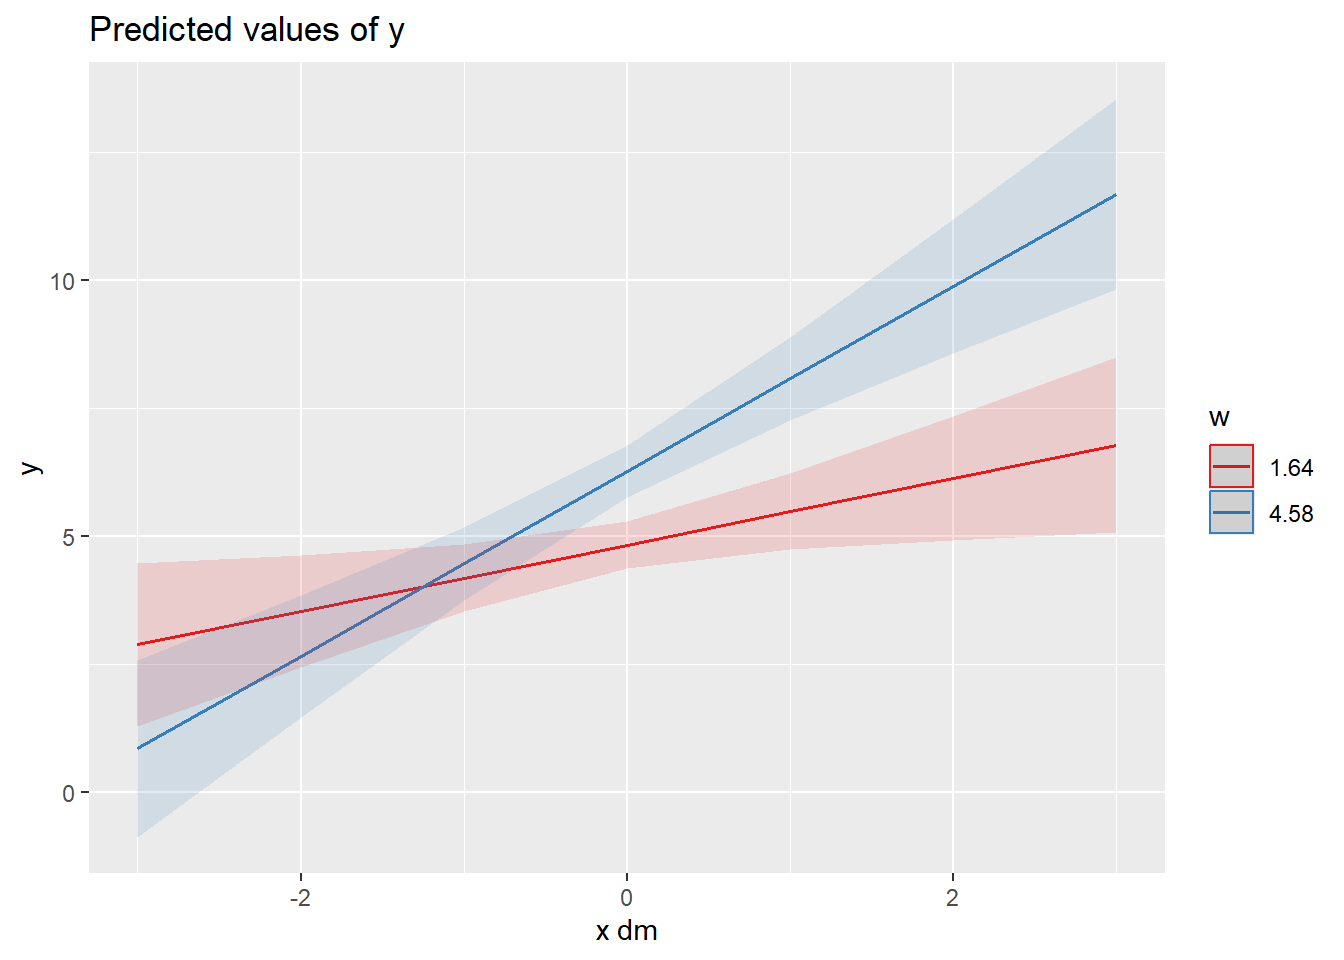
\includegraphics[keepaspectratio]{02-Descriptive-Statistics_files/figure-pdf/unnamed-chunk-19-1.pdf}}

\begin{Shaded}
\begin{Highlighting}[]
\FunctionTok{hist}\NormalTok{(mehrebenen\_stats}\SpecialCharTok{$}\NormalTok{mean[,}\StringTok{"b"}\NormalTok{])}
\end{Highlighting}
\end{Shaded}

\pandocbounded{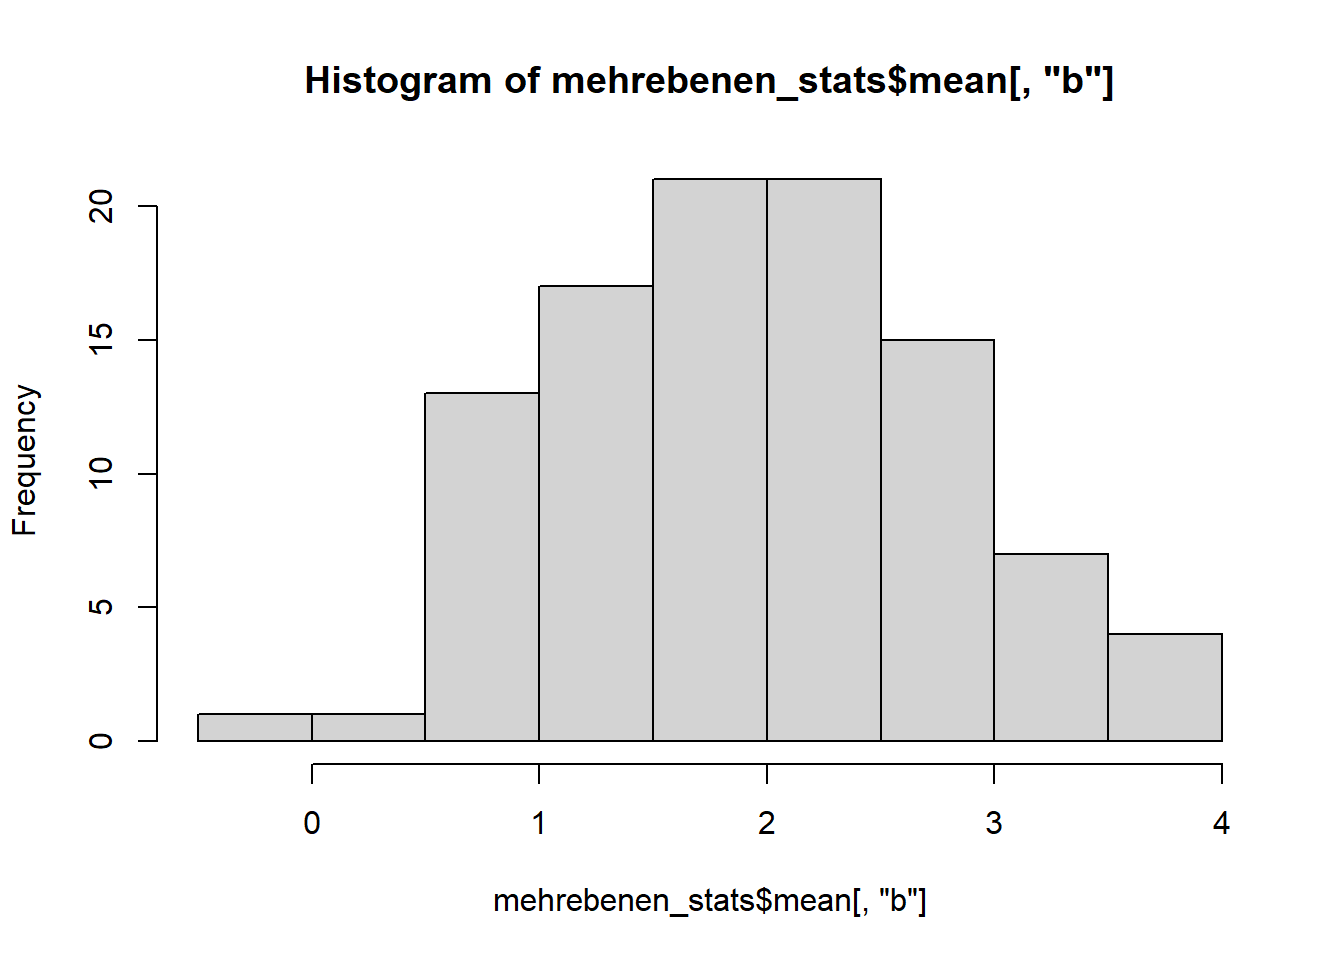
\includegraphics[keepaspectratio]{02-Descriptive-Statistics_files/figure-pdf/unnamed-chunk-19-2.pdf}}

\begin{Shaded}
\begin{Highlighting}[]
\FunctionTok{hist}\NormalTok{(mehrebenen\_stats}\SpecialCharTok{$}\NormalTok{mean[,}\StringTok{"c"}\NormalTok{])}
\end{Highlighting}
\end{Shaded}

\pandocbounded{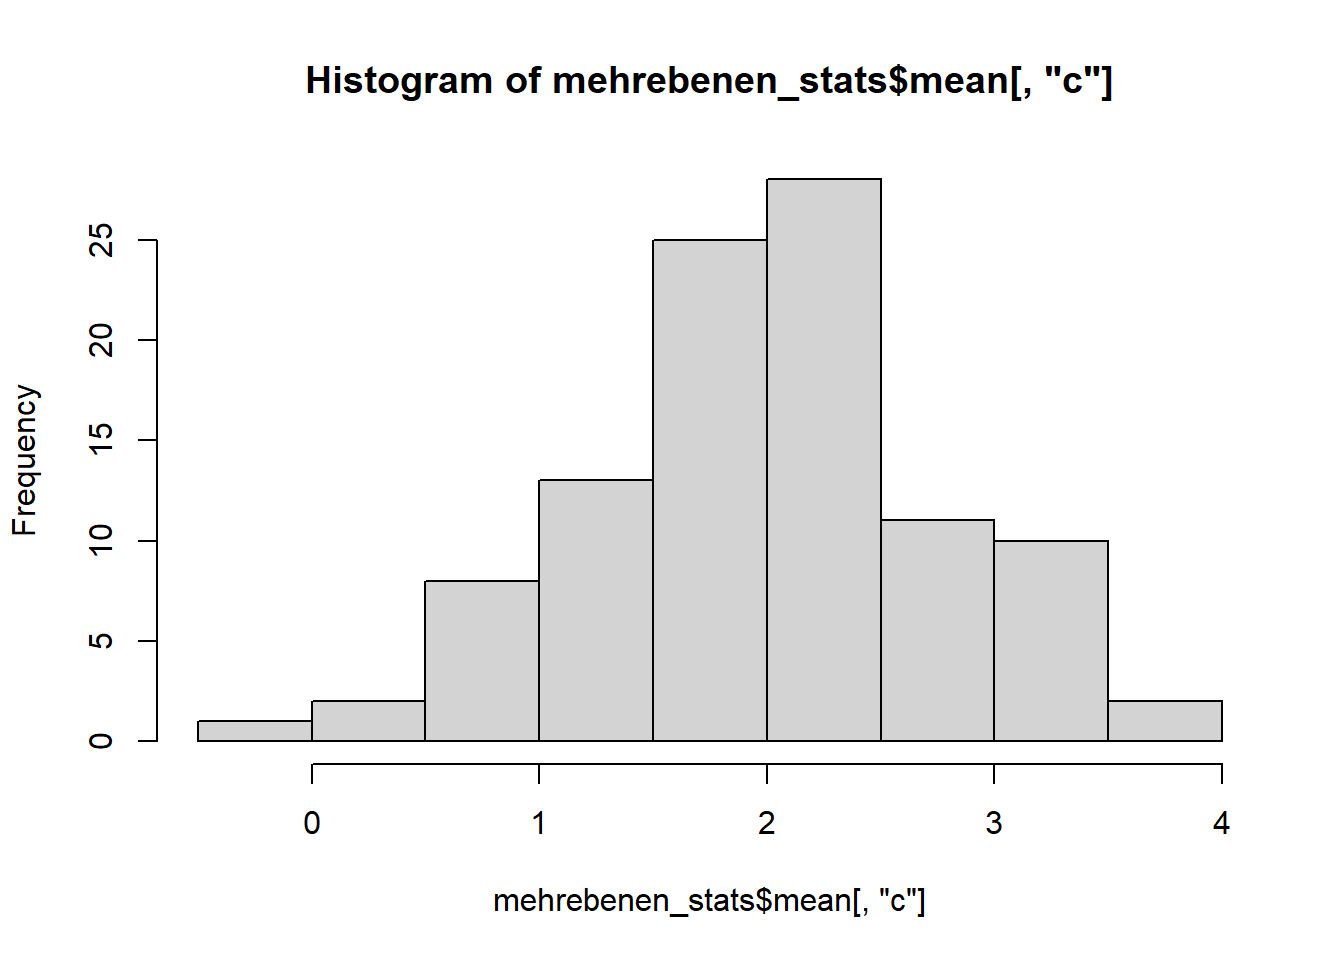
\includegraphics[keepaspectratio]{02-Descriptive-Statistics_files/figure-pdf/unnamed-chunk-19-3.pdf}}

Alle Variablen scheinen vom Histogram her hinreichend normalverteilt.

\subsubsection{Standardabweichungen}\label{standardabweichungen}

Ganz ähnlich wie mit Mittelwerten verfahren wir für die
Standardabweichung, nur dass wir hier als Funktion
\texttt{\textasciitilde{}sd(.x,\ na.rm\ =\ TRUE)} verwenden. Ersetzt
auch hier im folgenden Code in der Klammer von \texttt{c()} die
Variablennamen mit denen, die euch interessieren, hier sowohl die
täglichen als auch Baselinevariablen. Die Baselinevariable ``w'' zeigt
hier keine SD mit dieser Berechnung und muss separat berechnet werden.

\begin{Shaded}
\begin{Highlighting}[]
\NormalTok{standardabweichung }\OtherTok{\textless{}{-}}\NormalTok{ mehrebenen\_stats}\SpecialCharTok{$}\NormalTok{sd }\SpecialCharTok{|\textgreater{}} 
  \FunctionTok{as\_tibble}\NormalTok{() }\SpecialCharTok{|\textgreater{}} 
  \FunctionTok{summarise}\NormalTok{(}\FunctionTok{across}\NormalTok{(}\FunctionTok{c}\NormalTok{(a, b, c), }\SpecialCharTok{\textasciitilde{}}\FunctionTok{mean}\NormalTok{(.x, }\AttributeTok{na.rm =} \ConstantTok{TRUE}\NormalTok{)))}
\NormalTok{standardabweichung}
\end{Highlighting}
\end{Shaded}

\begin{verbatim}
# A tibble: 1 x 3
      a     b     c
  <dbl> <dbl> <dbl>
1 0.688 0.696 0.755
\end{verbatim}

\subsubsection{Korrelationen}\label{korrelationen}

Wir wollen eine Korrelationstabelle, in der wir auf einen Blick sowohl
die Zwischen-Person-Korrelationen als auch die
Inner-Person-Korrelationen sehen. Die \texttt{statsBy()} Funktion, die
wir bereits aufgerufen haben, gibt uns beides separat aus. und

\begin{Shaded}
\begin{Highlighting}[]
\NormalTok{mehrebenen\_stats}\SpecialCharTok{$}\NormalTok{rbg }\SpecialCharTok{|\textgreater{}} \FunctionTok{round}\NormalTok{(}\DecValTok{2}\NormalTok{) }\CommentTok{\# Zwischen Person Kor.}
\end{Highlighting}
\end{Shaded}

\begin{verbatim}
     a.bg b.bg c.bg
a.bg 1.00 0.32 0.39
b.bg 0.32 1.00 0.29
c.bg 0.39 0.29 1.00
\end{verbatim}

\begin{Shaded}
\begin{Highlighting}[]
\NormalTok{mehrebenen\_stats}\SpecialCharTok{$}\NormalTok{rwg }\SpecialCharTok{|\textgreater{}} \FunctionTok{round}\NormalTok{(}\DecValTok{2}\NormalTok{) }\CommentTok{\# Inner Person Kor.}
\end{Highlighting}
\end{Shaded}

\begin{verbatim}
     a.wg b.wg c.wg
a.wg 1.00 0.22 0.25
b.wg 0.22 1.00 0.29
c.wg 0.25 0.29 1.00
\end{verbatim}

Wir erhalten im unteren Dreieck die Inner-Person-Korrelationen, und im
oberen Dreieck die Zwischen-Person-Korrelationen.

\bookmarksetup{startatroot}

\chapter{Kapitel 4: Hypothesentests - Teil
1}\label{kapitel-4-hypothesentests---teil-1}

In diesem Kapitel verwenden wir verschiedene Regressionsmodelle die zur
Überprüfung von Hypothesen eingesetzt werden.

\begin{itemize}
\tightlist
\item
  Random Intercept Modell / Null-Model
\item
  Random Intercept, fixed slope Modell
\item
  Random intercept, random slope Modell
\item
  Erweiterung um Level-2 Prädiktoren
\end{itemize}

\section{Vorbereitung}\label{vorbereitung}

Install packages

\begin{Shaded}
\begin{Highlighting}[]
\ControlFlowTok{if}\NormalTok{ (}\SpecialCharTok{!}\FunctionTok{require}\NormalTok{(}\StringTok{"pacman"}\NormalTok{)) }\FunctionTok{install.packages}\NormalTok{(}\StringTok{"pacman"}\NormalTok{)}
\end{Highlighting}
\end{Shaded}

\begin{verbatim}
Lade nötiges Paket: pacman
\end{verbatim}

\begin{Shaded}
\begin{Highlighting}[]
\NormalTok{pacman}\SpecialCharTok{::}\FunctionTok{p\_load}\NormalTok{(lmerTest, haven, brms, psych,}
\NormalTok{               sjmisc, sjPlot, sjlabelled, writexl, broom.mixed, qgraph,}
\NormalTok{               tidyverse, multilevelTools, parameters)}
\end{Highlighting}
\end{Shaded}

\section{Daten einlesen}\label{daten-einlesen-1}

\begin{Shaded}
\begin{Highlighting}[]
\FunctionTok{load}\NormalTok{(}\StringTok{"../data/df\_example1.RData"}\NormalTok{)}
\FunctionTok{load}\NormalTok{(}\StringTok{"../data/df\_example1c.RData"}\NormalTok{)}
\end{Highlighting}
\end{Shaded}

Für diese Einheit verwenden wir den folgenden Datensatz
(data.frame/tibble):

\begin{itemize}
\tightlist
\item
  df\_example1: Alle Skalenscores im Long Format, mit
  personen-zentrierten Variablenvarianten (``\_dm'') und
  Personen-Mittelwerten der täglich gemessenenen Variablen (``\_gm'').
  Struktur des Datensatzes kann man sich ansehen mit \texttt{head()}
  oder \texttt{print()}.
\end{itemize}

\begin{Shaded}
\begin{Highlighting}[]
\FunctionTok{head}\NormalTok{(df\_example1)}
\end{Highlighting}
\end{Shaded}

\begin{verbatim}
# A tibble: 6 x 10
  id        y     m     x    y_dm   m_dm    x_dm  y_gm  m_gm  x_gm
  <fct> <dbl> <dbl> <dbl>   <dbl>  <dbl>   <dbl> <dbl> <dbl> <dbl>
1 1      4.00  4.77 2.37  -0.302   0.895  0.685   4.31  3.87  1.68
2 1      4.93  2.51 0.749  0.620  -1.36  -0.932   4.31  3.87  1.68
3 1      4.60  3.10 1.40   0.293  -0.777 -0.286   4.31  3.87  1.68
4 1      4.29  4.61 1.86  -0.0194  0.736  0.179   4.31  3.87  1.68
5 1      4.18  4.55 2.29  -0.122   0.674  0.607   4.31  3.87  1.68
6 1      3.63  3.59 1.70  -0.674  -0.285  0.0156  4.31  3.87  1.68
\end{verbatim}

Im Folgenden betrachten wir ein Modell in dem y durch x vorhergesagt
wird.

\section{Random Intercept Modell /
Null-Model}\label{random-intercept-modell-null-model}

Die Funktion lmer() benötigt zwei Argumente, (a) die Formel und (b) den
Datensatz. Zum Aufbau und Details der Formeln s. Folien.

Level 1: \(y_{ij} = \beta_{0j} + e_{ij}\)

Level 2 (random intercept): \(\beta_{0j} = \gamma_{00} + u_{0j}\)

\begin{Shaded}
\begin{Highlighting}[]
\NormalTok{nullmodel }\OtherTok{\textless{}{-}} \FunctionTok{lmer}\NormalTok{(y }\SpecialCharTok{\textasciitilde{}}\NormalTok{ (}\DecValTok{1} \SpecialCharTok{|}\NormalTok{ id), }\AttributeTok{data =}\NormalTok{ df\_example1)}
\end{Highlighting}
\end{Shaded}

Zur Ansicht der Ergebnisse haben wir zwei Optionen: Den
\texttt{summary()} Befehl - die Standardansicht, wie von den
Paketautoren implementiert, den \texttt{tidy()} Befehl aus dem
broom-Package, und den \texttt{model\_parameters()} Befehl aus dem
parameters Package. tidy() und model\_parameters() Funktionsoutputs
könnten nach Excel/Word exportiert werden mittels der
\texttt{write\_xlsx()} Funktion, oder indem das Notebook als .docx
``gerendert'' (ausgegeben) wird.

\begin{Shaded}
\begin{Highlighting}[]
\FunctionTok{summary}\NormalTok{(nullmodel)}
\end{Highlighting}
\end{Shaded}

\begin{verbatim}
Linear mixed model fit by REML. t-tests use Satterthwaite's method [
lmerModLmerTest]
Formula: y ~ (1 | id)
   Data: df_example1

REML criterion at convergence: 2742.9

Scaled residuals: 
    Min      1Q  Median      3Q     Max 
-6.1492 -0.5420 -0.0369  0.5543  4.6493 

Random effects:
 Groups   Name        Variance Std.Dev.
 id       (Intercept) 0.6902   0.8308  
 Residual             0.7164   0.8464  
Number of obs: 1000, groups:  id, 100

Fixed effects:
            Estimate Std. Error       df t value Pr(>|t|)    
(Intercept)  5.36755    0.08728 99.00000    61.5   <2e-16 ***
---
Signif. codes:  0 '***' 0.001 '**' 0.01 '*' 0.05 '.' 0.1 ' ' 1
\end{verbatim}

\begin{Shaded}
\begin{Highlighting}[]
\FunctionTok{tidy}\NormalTok{(nullmodel)}
\end{Highlighting}
\end{Shaded}

\begin{verbatim}
# A tibble: 3 x 8
  effect   group    term            estimate std.error statistic    df   p.value
  <chr>    <chr>    <chr>              <dbl>     <dbl>     <dbl> <dbl>     <dbl>
1 fixed    <NA>     (Intercept)        5.37     0.0873      61.5  99.0  1.10e-80
2 ran_pars id       sd__(Intercept)    0.831   NA           NA    NA   NA       
3 ran_pars Residual sd__Observation    0.846   NA           NA    NA   NA       
\end{verbatim}

\begin{Shaded}
\begin{Highlighting}[]
\FunctionTok{model\_parameters}\NormalTok{(nullmodel) }\SpecialCharTok{|\textgreater{}} \FunctionTok{print\_html}\NormalTok{()}
\end{Highlighting}
\end{Shaded}

\begingroup
\fontsize{12.0pt}{14.4pt}\selectfont
\setlength{\LTpost}{0mm}
\begin{longtable*}{lccccc}
\caption*{
{\large Model Summary}
} \\ 
\toprule
Parameter & Coefficient & SE & 95\% CI & t(997) & p \\ 
\midrule\addlinespace[2.5pt]
\multicolumn{6}{l}{Fixed Effects } \\[2.5pt] 
\midrule\addlinespace[2.5pt]
{(Intercept)} & 5.37 & 0.09 & (5.20, 5.54) & 61.50 & < .001 \\ 
\midrule\addlinespace[2.5pt]
\multicolumn{6}{l}{Random Effects } \\[2.5pt] 
\midrule\addlinespace[2.5pt]
{SD (Intercept: id)} & 0.83 &  &  &  &  \\ 
{SD (Residual)} & 0.85 &  &  &  &  \\ 
\bottomrule
\end{longtable*}
\begin{minipage}{\linewidth}
\\
\end{minipage}
\endgroup

Im Seminar verwenden wir den Output von model\_parameters(), weil er
eine recht gut formatierte Übersicht gibt.

\subsection{ICC}\label{icc}

Aus dem Null-Model wird der ICC bestimmt. Dies haben wir in der
vorhergehenden

ICC: \(\frac{\tau_{00}}{\tau_{00}+\tau_{ij}}\), \(\tau\) gibt die
Varianz des jewiligen Koeffizienten an.

Wir können dies aus dem Modelloutput nehmen und berechnen:

\begin{Shaded}
\begin{Highlighting}[]
\NormalTok{modelsummary }\OtherTok{\textless{}{-}} \FunctionTok{model\_parameters}\NormalTok{(nullmodel)}
\NormalTok{tau00 }\OtherTok{\textless{}{-}}\NormalTok{ modelsummary}\SpecialCharTok{$}\NormalTok{Coefficient[modelsummary}\SpecialCharTok{$}\NormalTok{Parameter }\SpecialCharTok{==} \StringTok{"SD (Intercept)"}\NormalTok{]}\SpecialCharTok{\^{}}\DecValTok{2}
\NormalTok{tauij }\OtherTok{\textless{}{-}}\NormalTok{ modelsummary}\SpecialCharTok{$}\NormalTok{Coefficient[modelsummary}\SpecialCharTok{$}\NormalTok{Parameter }\SpecialCharTok{==} \StringTok{"SD (Observations)"}\NormalTok{]}\SpecialCharTok{\^{}}\DecValTok{2}
\NormalTok{tau00 }\SpecialCharTok{/}\NormalTok{ (tau00}\SpecialCharTok{+}\NormalTok{tauij)}
\end{Highlighting}
\end{Shaded}

\begin{verbatim}
[1] 0.4906711
\end{verbatim}

\begin{Shaded}
\begin{Highlighting}[]
\CommentTok{\# performance::icc(nullmodel) \# Alternativfunktion}
\end{Highlighting}
\end{Shaded}

\subsection{Visualisierung}\label{visualisierung}

Wir können uns die Analysen visualisieren, hier zur reduzierten
visuellen Komplexität nur auf Basis der ersten 20 Personen (ID 1-20.)

\begin{verbatim}
Warning: Using `size` aesthetic for lines was deprecated in ggplot2 3.4.0.
i Please use `linewidth` instead.
\end{verbatim}

\begin{verbatim}
`geom_smooth()` using formula = 'y ~ x'
\end{verbatim}

\pandocbounded{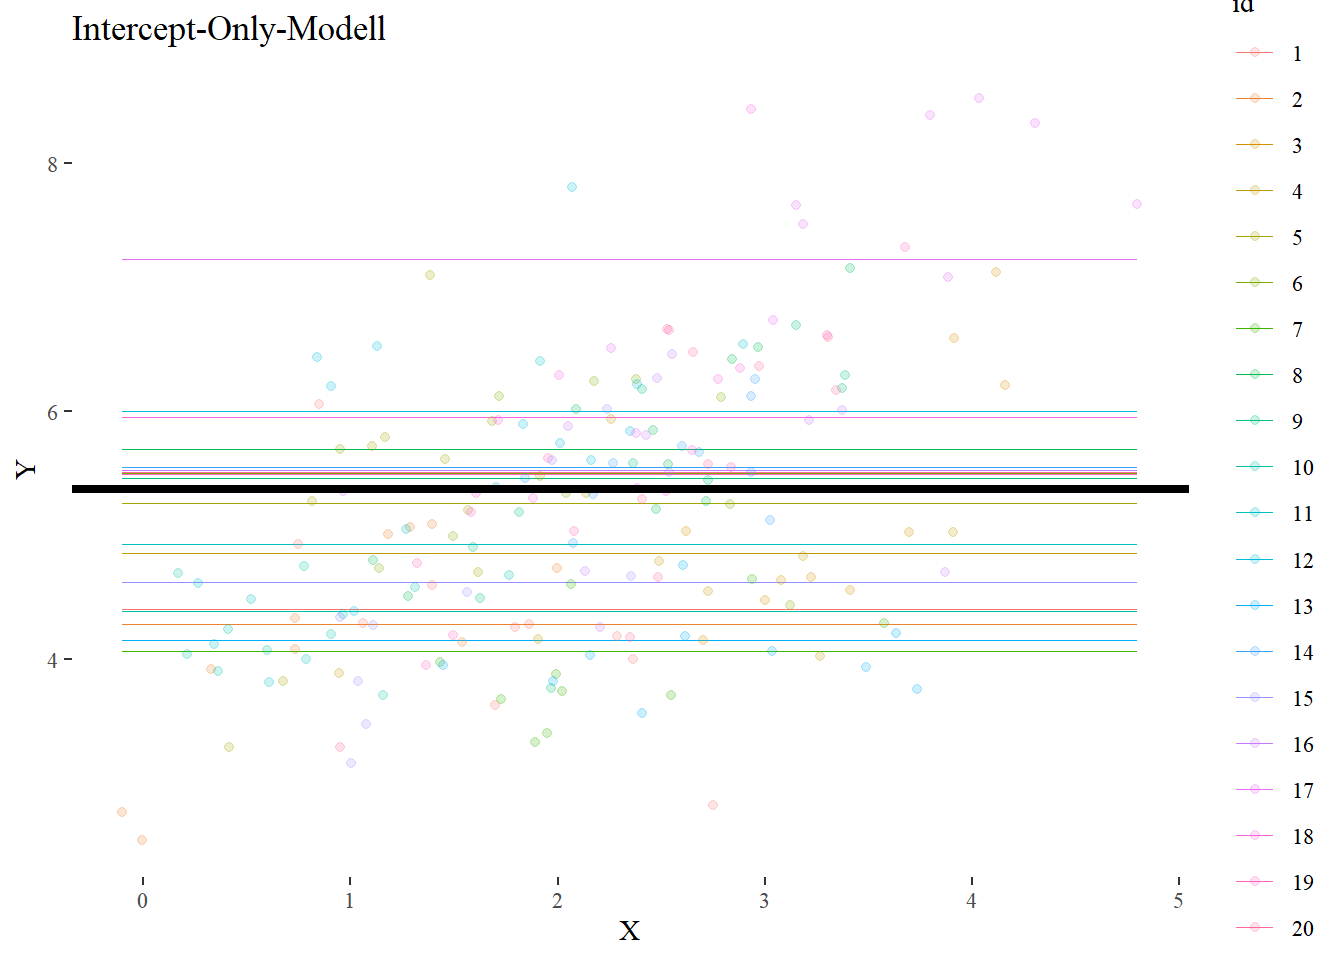
\includegraphics[keepaspectratio]{03-Hypotheses-Tests_files/figure-pdf/unnamed-chunk-9-1.pdf}}

Oder zwei Personen, um uns die einzelnen Punkte auch anschauen zu
können:

\begin{Shaded}
\begin{Highlighting}[]
\FunctionTok{ggplot}\NormalTok{(}\AttributeTok{data =}\NormalTok{ df\_example1 }\SpecialCharTok{|\textgreater{}} \FunctionTok{filter}\NormalTok{(id }\SpecialCharTok{\%in\%} \FunctionTok{c}\NormalTok{(}\DecValTok{1}\NormalTok{, }\DecValTok{16}\NormalTok{)), }\FunctionTok{aes}\NormalTok{(}
  \AttributeTok{x =}\NormalTok{ x,}
  \AttributeTok{y =}\NormalTok{ predicted\_ri,}
  \AttributeTok{colour =}\NormalTok{ id}
\NormalTok{)) }\SpecialCharTok{+}
  \FunctionTok{geom\_smooth}\NormalTok{(}\AttributeTok{method =} \StringTok{"lm"}\NormalTok{, }\AttributeTok{fullrange =} \ConstantTok{TRUE}\NormalTok{, }\AttributeTok{se =}\NormalTok{ F, }\AttributeTok{size =} \DecValTok{1}\NormalTok{) }\SpecialCharTok{+}
  \FunctionTok{geom\_jitter}\NormalTok{(}\FunctionTok{aes}\NormalTok{(}\AttributeTok{y =}\NormalTok{ y), }\AttributeTok{alpha =}\NormalTok{ .}\DecValTok{5}\NormalTok{, }\AttributeTok{size =} \FloatTok{2.5}\NormalTok{) }\SpecialCharTok{+}
  \FunctionTok{labs}\NormalTok{(}\AttributeTok{x =}\NormalTok{ xlabel, }\AttributeTok{y =}\NormalTok{ ylabel) }\SpecialCharTok{+}
  \FunctionTok{ggtitle}\NormalTok{(}\StringTok{"Intercept{-}Only{-}Modell"}\NormalTok{) }\SpecialCharTok{+}
  \FunctionTok{scale\_colour\_discrete}\NormalTok{() }\SpecialCharTok{+}
  \FunctionTok{geom\_abline}\NormalTok{(}\AttributeTok{intercept =} \FunctionTok{fixef}\NormalTok{(nullmodel), }\AttributeTok{slope =} \DecValTok{0}\NormalTok{, }\AttributeTok{size =} \FloatTok{1.5}\NormalTok{) }\SpecialCharTok{+}
\NormalTok{  ggthemes}\SpecialCharTok{::}\FunctionTok{theme\_tufte}\NormalTok{()}
\end{Highlighting}
\end{Shaded}

\begin{verbatim}
`geom_smooth()` using formula = 'y ~ x'
\end{verbatim}

\pandocbounded{\includegraphics[keepaspectratio]{03-Hypotheses-Tests_files/figure-pdf/unnamed-chunk-10-1.pdf}}

\section{Random Intercept, fixed slope
Modell}\label{random-intercept-fixed-slope-modell}

Als nächstes bauen wir den Prädiktor x ein. Wir verwenden hier die
zentrierte Variable ``\texttt{\_dm}'' um Inner-Person Effekte zu
berechnen.

Level 1: \(y_{ij} = \beta_{0j} + \beta_{1j}*X_{ij} + e_{ij}\)

Level 2 (random intercept): \(\beta_{0j} = \gamma_{00} + u_{0j}\)

Level 2 (fixed effect only): \(\beta'_{1j} = \gamma'_{10}\)

\begin{Shaded}
\begin{Highlighting}[]
\NormalTok{ri.fs\_modell }\OtherTok{\textless{}{-}} \FunctionTok{lmer}\NormalTok{(y }\SpecialCharTok{\textasciitilde{}}\NormalTok{ x\_dm }\SpecialCharTok{+}\NormalTok{ (}\DecValTok{1} \SpecialCharTok{|}\NormalTok{ id), }\AttributeTok{data =}\NormalTok{ df\_example1)}
\end{Highlighting}
\end{Shaded}

\begin{Shaded}
\begin{Highlighting}[]
\FunctionTok{model\_parameters}\NormalTok{(ri.fs\_modell) }\SpecialCharTok{|\textgreater{}} \FunctionTok{print\_html}\NormalTok{()}
\end{Highlighting}
\end{Shaded}

\begingroup
\fontsize{12.0pt}{14.4pt}\selectfont
\setlength{\LTpost}{0mm}
\begin{longtable*}{lccccc}
\caption*{
{\large Model Summary}
} \\ 
\toprule
Parameter & Coefficient & SE & 95\% CI & t(996) & p \\ 
\midrule\addlinespace[2.5pt]
\multicolumn{6}{l}{Fixed Effects } \\[2.5pt] 
\midrule\addlinespace[2.5pt]
{(Intercept)} & 5.37 & 0.09 & (5.20, 5.54) & 61.50 & < .001 \\ 
{x dm} & 0.44 & 0.04 & (0.36, 0.51) & 11.63 & < .001 \\ 
\midrule\addlinespace[2.5pt]
\multicolumn{6}{l}{Random Effects } \\[2.5pt] 
\midrule\addlinespace[2.5pt]
{SD (Intercept: id)} & 0.84 &  &  &  &  \\ 
{SD (Residual)} & 0.79 &  &  &  &  \\ 
\bottomrule
\end{longtable*}
\begin{minipage}{\linewidth}
\\
\end{minipage}
\endgroup

\subsection{Visualisierung}\label{visualisierung-1}

\begin{verbatim}
`geom_smooth()` using formula = 'y ~ x'
\end{verbatim}

\pandocbounded{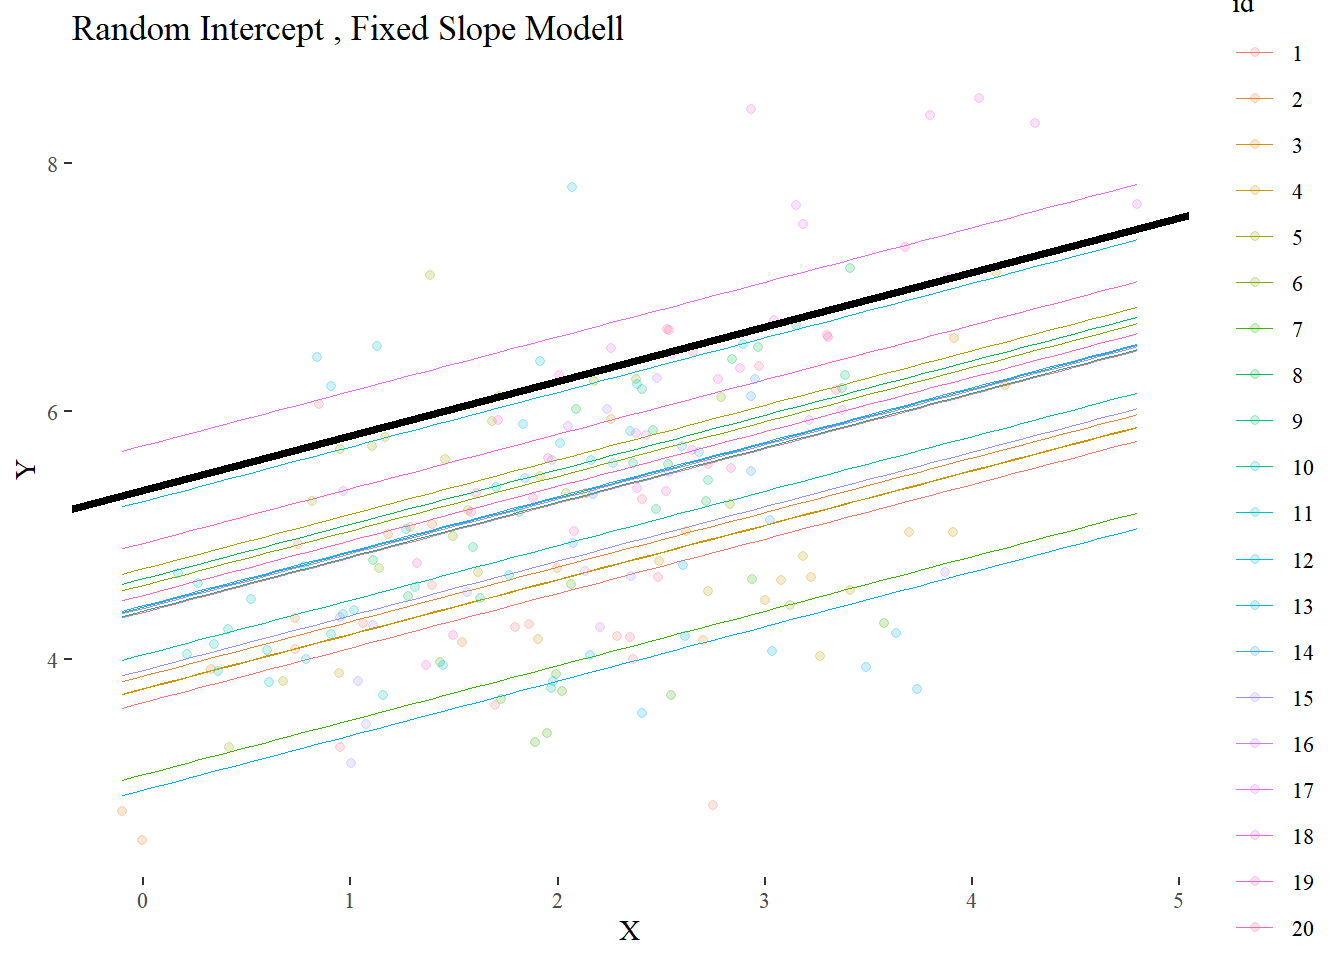
\includegraphics[keepaspectratio]{03-Hypotheses-Tests_files/figure-pdf/unnamed-chunk-13-1.pdf}}

\section{Random intercept, random slope
Modell}\label{random-intercept-random-slope-modell}

Als nächstes fügen wir den random slope der Prädiktorvariable x\_dm
hinzu, in dem wir die random effect Struktur erweitern - ``(1 + x\_dm
\textbar{} id)''.

Level 1:
\(y_{ij} = \beta_{0j} + \beta_{1j}*(X_{ij}-\overline{X_j}) + e_{ij}\)

Level 2 (random intercept): \(\beta_{0j} = \gamma_{00} + u_{0j}\)

Level 2: \(\beta'_{1j} = \gamma'_{10}\)

\begin{Shaded}
\begin{Highlighting}[]
\NormalTok{ri.rs\_modell }\OtherTok{\textless{}{-}} \FunctionTok{lmer}\NormalTok{(y }\SpecialCharTok{\textasciitilde{}}\NormalTok{ x\_dm }\SpecialCharTok{+}\NormalTok{ (}\DecValTok{1} \SpecialCharTok{+}\NormalTok{ x\_dm }\SpecialCharTok{|}\NormalTok{ id), }\AttributeTok{data =}\NormalTok{ df\_example1)}
\FunctionTok{model\_parameters}\NormalTok{(ri.rs\_modell) }\SpecialCharTok{|\textgreater{}} \FunctionTok{print\_html}\NormalTok{()}
\end{Highlighting}
\end{Shaded}

\begingroup
\fontsize{12.0pt}{14.4pt}\selectfont
\setlength{\LTpost}{0mm}
\begin{longtable*}{lccccc}
\caption*{
{\large Model Summary}
} \\ 
\toprule
Parameter & Coefficient & SE & 95\% CI & t(994) & p \\ 
\midrule\addlinespace[2.5pt]
\multicolumn{6}{l}{Fixed Effects } \\[2.5pt] 
\midrule\addlinespace[2.5pt]
{(Intercept)} & 5.37 & 0.09 & (5.20, 5.54) & 61.50 & < .001 \\ 
{x dm} & 0.42 & 0.07 & (0.28, 0.56) & 5.88 & < .001 \\ 
\midrule\addlinespace[2.5pt]
\multicolumn{6}{l}{Random Effects } \\[2.5pt] 
\midrule\addlinespace[2.5pt]
{SD (Intercept: id)} & 0.85 &  &  &  &  \\ 
{SD (x\_dm: id)} & 0.63 &  &  &  &  \\ 
{Cor (Intercept\textasciitilde{}x\_dm: id)} & 0.20 &  &  &  &  \\ 
{SD (Residual)} & 0.65 &  &  &  &  \\ 
\bottomrule
\end{longtable*}
\begin{minipage}{\linewidth}
\\
\end{minipage}
\endgroup

\subsection{Visualisierung}\label{visualisierung-2}

\begin{verbatim}
`geom_smooth()` using formula = 'y ~ x'
\end{verbatim}

\pandocbounded{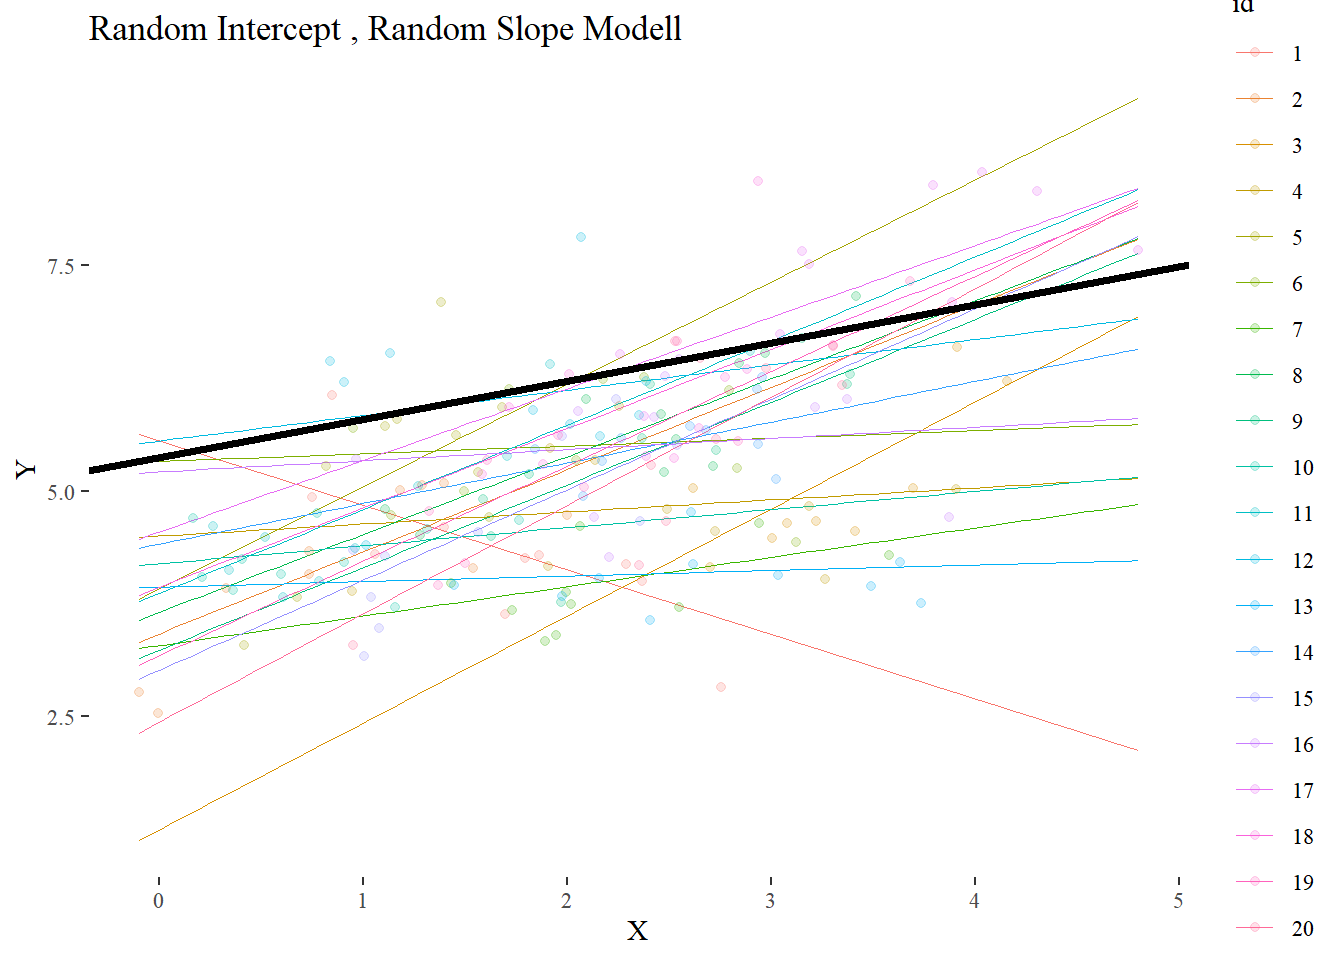
\includegraphics[keepaspectratio]{03-Hypotheses-Tests_files/figure-pdf/unnamed-chunk-15-1.pdf}}

\section{Level-2 Prädiktoren}\label{level-2-pruxe4diktoren}

Als nächstes fügen wir einen Level-2 Prädiktor hinzu, der pro Person nur
einmal gemessen wurde. Dabei handelt es sich für gewöhnlich um (1)
Variablen, bei denen wir nicht an täglichen Schwankungen interessiert
sind, wie soziodemografischen oder Persönlichkeitsvariablen, oder (2)
den Mittelwert der Personen auf einer täglich gemessenen Variable. Im
Beispiel verwenden wir (2), ``x\_gm''.

Level 1:
\(y_{ij} = \beta_{0j} + \beta_{1j}*(X_{ij}-\overline{X_j}) + \beta_{2j}*\overline{X_j} + e_{ij}\)

Level 2 (random intercept): \(\beta_{0j} = \gamma_{00} + u_{0j}\) Level
2 (random slope for x): \(\beta_{1j} = \gamma_{10} + u_{2j}\)

\begin{Shaded}
\begin{Highlighting}[]
\NormalTok{ri.rs\_l2\_modell }\OtherTok{\textless{}{-}} \FunctionTok{lmer}\NormalTok{(y }\SpecialCharTok{\textasciitilde{}}\NormalTok{ x\_dm }\SpecialCharTok{+}\NormalTok{ x\_gm }\SpecialCharTok{+}\NormalTok{ (}\DecValTok{1} \SpecialCharTok{+}\NormalTok{ x\_dm }\SpecialCharTok{|}\NormalTok{ id), }\AttributeTok{data =}\NormalTok{ df\_example1)}
\FunctionTok{model\_parameters}\NormalTok{(ri.rs\_l2\_modell) }\SpecialCharTok{|\textgreater{}} \FunctionTok{print\_html}\NormalTok{()}
\end{Highlighting}
\end{Shaded}

\begingroup
\fontsize{12.0pt}{14.4pt}\selectfont
\setlength{\LTpost}{0mm}
\begin{longtable*}{lccccc}
\caption*{
{\large Model Summary}
} \\ 
\toprule
Parameter & Coefficient & SE & 95\% CI & t(993) & p \\ 
\midrule\addlinespace[2.5pt]
\multicolumn{6}{l}{Fixed Effects } \\[2.5pt] 
\midrule\addlinespace[2.5pt]
{(Intercept)} & 4.47 & 0.19 & (4.09, 4.84) & 23.30 & < .001 \\ 
{x dm} & 0.42 & 0.07 & (0.28, 0.56) & 5.85 & < .001 \\ 
{x gm} & 0.43 & 0.08 & (0.26, 0.59) & 5.13 & < .001 \\ 
\midrule\addlinespace[2.5pt]
\multicolumn{6}{l}{Random Effects } \\[2.5pt] 
\midrule\addlinespace[2.5pt]
{SD (Intercept: id)} & 0.75 &  &  &  &  \\ 
{SD (x\_dm: id)} & 0.63 &  &  &  &  \\ 
{Cor (Intercept\textasciitilde{}x\_dm: id)} & 0.17 &  &  &  &  \\ 
{SD (Residual)} & 0.65 &  &  &  &  \\ 
\bottomrule
\end{longtable*}
\begin{minipage}{\linewidth}
\\
\end{minipage}
\endgroup

\section{Übung}\label{uxfcbung-1}

Wir arbeiten in der Übung mit einem neuen Datensatz.

Mache dich mit ihm vertraut. Diesmal benutzen wir einen Datensatz in dem
die Variablen ``labelled'' sind, also Beschriftungen haben. Wir können
die Labels mit \texttt{get\_label()} oder \texttt{view\_df()} abrufen.

\begin{Shaded}
\begin{Highlighting}[]
\FunctionTok{load}\NormalTok{(}\StringTok{"../data/df\_example\_cli.RData"}\NormalTok{)}

\FunctionTok{head}\NormalTok{(df\_example\_cli)}
\end{Highlighting}
\end{Shaded}

\begin{verbatim}
# A tibble: 6 x 10
     id illtask negativ support illtask_dm negativ_dm illtask_gm negativ_gm
  <int>   <dbl>   <dbl>   <dbl>      <dbl>      <dbl>      <dbl>      <dbl>
1     1    1.19    1.83    3.45    -1.30      -0.0154       2.49       1.84
2     1    1.72    1.63    3.45    -0.769     -0.208        2.49       1.84
3     1    3.15    1.25    3.45     0.661     -0.591        2.49       1.84
4     1    2.37    1.58    3.45    -0.116     -0.257        2.49       1.84
5     1    2.56    2.91    3.45     0.0702     1.07         2.49       1.84
6     2    1.34    2.11    2.11     0.281     -0.491        1.06       2.60
# i 2 more variables: negativ_dm_l1 <dbl>, day <int>
\end{verbatim}

\begin{Shaded}
\begin{Highlighting}[]
\FunctionTok{view\_df}\NormalTok{(df\_example\_cli)}
\end{Highlighting}
\end{Shaded}

\begin{longtable}[]{@{}lllll@{}}
\caption{Data frame: df\_example\_cli}\tabularnewline
\toprule\noalign{}
\endfirsthead
\endhead
\bottomrule\noalign{}
\endlastfoot
ID & Name & Label & Values & Value Labels \\
1 & id & Personen-ID & \multicolumn{2}{l@{}}{%
\emph{range: 1-100}} \\
2 & illtask & Daily Illegitimate Tasks & \multicolumn{2}{l@{}}{%
\emph{range: -1.9-5.6}} \\
3 & negativ & Daily Negative Affect & \multicolumn{2}{l@{}}{%
\emph{range: -0.2-7.7}} \\
4 & support & Coworker support & \multicolumn{2}{l@{}}{%
\emph{range: 1.4-4.5}} \\
5 & illtask\_dm & Illegitimate Tasks (person-mean centered) &
\multicolumn{2}{l@{}}{%
\emph{range: -2.1-2.3}} \\
6 & negativ\_dm & Neg. Affect (person-mean centered) &
\multicolumn{2}{l@{}}{%
\emph{range: -2.0-2.7}} \\
7 & illtask\_gm & Illegitimate Tasks (person average) &
\multicolumn{2}{l@{}}{%
\emph{range: -0.7-4.7}} \\
8 & negativ\_gm & Neg. Affect (person average) & \multicolumn{2}{l@{}}{%
\emph{range: 0.8-5.0}} \\
9 & negativ\_dm\_l1 & Previous-day Neg. Affect & \multicolumn{2}{l@{}}{%
\emph{range: -2.0-2.7}} \\
10 & day & Tag (1-10) & \multicolumn{2}{l@{}}{%
\emph{range: 1-10}} \\
\end{longtable}

\begin{Shaded}
\begin{Highlighting}[]
\CommentTok{\# alternativ}
\CommentTok{\#get\_label(df\_example\_cli)}
\end{Highlighting}
\end{Shaded}

Berechne Modelle mit denen du die folgenden Hypothesen testest:

Hypothese 1: Tägliche illegitime Aufgaben hängen positiv mit täglichem
negativem Affekt zusammen.

Teste zunächst ein Random intercept, fixed slope Modell, und dann ein
Random Intercept, Random Slope Modell. Urteile, ob die Hypothese
angenommen oder verworfen werden sollten.

\begin{tcolorbox}[enhanced jigsaw, opacitybacktitle=0.6, left=2mm, colback=white, rightrule=.15mm, title=\textcolor{quarto-callout-tip-color}{\faLightbulb}\hspace{0.5em}{Lösung}, breakable, leftrule=.75mm, colframe=quarto-callout-tip-color-frame, toptitle=1mm, toprule=.15mm, titlerule=0mm, arc=.35mm, bottomtitle=1mm, colbacktitle=quarto-callout-tip-color!10!white, coltitle=black, bottomrule=.15mm, opacityback=0]

\begin{Shaded}
\begin{Highlighting}[]
\NormalTok{ri.fs\_modell }\OtherTok{\textless{}{-}} \FunctionTok{lmer}\NormalTok{(negativ }\SpecialCharTok{\textasciitilde{}}\NormalTok{ illtask\_dm }\SpecialCharTok{+}\NormalTok{ (}\DecValTok{1} \SpecialCharTok{|}\NormalTok{ id), }\AttributeTok{data =}\NormalTok{ df\_example\_cli)}
\FunctionTok{parameters}\NormalTok{(ri.fs\_modell) }\SpecialCharTok{|\textgreater{}} \FunctionTok{print\_html}\NormalTok{()}
\end{Highlighting}
\end{Shaded}

\begin{verbatim}
Package 'merDeriv' needs to be installed to compute confidence intervals
  for random effect parameters.
\end{verbatim}

\begingroup
\fontsize{12.0pt}{14.4pt}\selectfont
\setlength{\LTpost}{0mm}
\begin{longtable*}{lccccc}
\caption*{
{\large Model Summary}
} \\ 
\toprule
Parameter & Coefficient & SE & 95\% CI & t(779) & p \\ 
\midrule\addlinespace[2.5pt]
\multicolumn{6}{l}{Fixed Effects } \\[2.5pt] 
\midrule\addlinespace[2.5pt]
{(Intercept)} & 2.73 & 0.07 & (2.59, 2.87) & 37.43 & < .001 \\ 
{illtask dm} & 0.30 & 0.04 & (0.23, 0.38) & 8.07 & < .001 \\ 
\midrule\addlinespace[2.5pt]
\multicolumn{6}{l}{Random Effects } \\[2.5pt] 
\midrule\addlinespace[2.5pt]
{SD (Intercept: id)} & 0.68 &  &  &  &  \\ 
{SD (Residual)} & 0.72 &  &  &  &  \\ 
\bottomrule
\end{longtable*}
\begin{minipage}{\linewidth}
\\
\end{minipage}
\endgroup

\begin{Shaded}
\begin{Highlighting}[]
\NormalTok{ri.rs\_modell }\OtherTok{\textless{}{-}} \FunctionTok{lmer}\NormalTok{(negativ }\SpecialCharTok{\textasciitilde{}}\NormalTok{ illtask\_dm }\SpecialCharTok{+}\NormalTok{ (}\DecValTok{1} \SpecialCharTok{+}\NormalTok{ illtask\_dm }\SpecialCharTok{|}\NormalTok{ id), }\AttributeTok{data =}\NormalTok{ df\_example\_cli)}
\FunctionTok{parameters}\NormalTok{(ri.rs\_modell) }\SpecialCharTok{|\textgreater{}} \FunctionTok{print\_html}\NormalTok{()}
\end{Highlighting}
\end{Shaded}

\begingroup
\fontsize{12.0pt}{14.4pt}\selectfont
\setlength{\LTpost}{0mm}
\begin{longtable*}{lccccc}
\caption*{
{\large Model Summary}
} \\ 
\toprule
Parameter & Coefficient & SE & 95\% CI & t(777) & p \\ 
\midrule\addlinespace[2.5pt]
\multicolumn{6}{l}{Fixed Effects } \\[2.5pt] 
\midrule\addlinespace[2.5pt]
{(Intercept)} & 2.73 & 0.07 & (2.59, 2.87) & 37.65 & < .001 \\ 
{illtask dm} & 0.32 & 0.05 & (0.22, 0.43) & 6.37 & < .001 \\ 
\midrule\addlinespace[2.5pt]
\multicolumn{6}{l}{Random Effects } \\[2.5pt] 
\midrule\addlinespace[2.5pt]
{SD (Intercept: id)} & 0.68 &  &  &  &  \\ 
{SD (illtask\_dm: id)} & 0.35 &  &  &  &  \\ 
{Cor (Intercept\textasciitilde{}illtask\_dm: id)} & 0.70 &  &  &  &  \\ 
{SD (Residual)} & 0.68 &  &  &  &  \\ 
\bottomrule
\end{longtable*}
\begin{minipage}{\linewidth}
\\
\end{minipage}
\endgroup

Die Hypothese 1 kann angenommen werden, da der Effekt von illegitimen
Aufgaben (\texttt{illtask\_dm}) signifikant positiv ist. Auch im
strengeren random Slopes Modell ist der Effekt weiterhin signifikant.

Wir können auch sehen, dass im Random Slopes Modell die
Konfidenzintervalle etwas breiter sind und der Standardfehler etwas
grösser sind als im Fixed Slopes Modell. In Random Slopes Modellen
können die Regressionskoeffizienten zwischen den Individuen variieren,
was zusätzliche Varianz in die Schätzungen einbringt. Diese zusätzliche
Unsicherheit führt dazu, dass sowohl die Standardfehler als auch die
Konfidenzintervalle grösser ausfallen als in Fixed Slopes Modellen, bei
denen die Steigung als konstant über alle Gruppen angenommen wird.
Dadurch reflektieren die größeren Intervalle die höhere Unsicherheit in
der Modellierung individueller Unterschiede in den Effekten.

\end{tcolorbox}

\bookmarksetup{startatroot}

\chapter{Kapitel 5: Hypothestentests 2 - Moderation und
Mediation}\label{kapitel-5-hypothestentests-2---moderation-und-mediation}

\begin{Shaded}
\begin{Highlighting}[]
\ControlFlowTok{if}\NormalTok{ (}\SpecialCharTok{!}\FunctionTok{require}\NormalTok{(}\StringTok{"pacman"}\NormalTok{)) }\FunctionTok{install.packages}\NormalTok{(}\StringTok{"pacman"}\NormalTok{)}
\end{Highlighting}
\end{Shaded}

\begin{verbatim}
Lade nötiges Paket: pacman
\end{verbatim}

\begin{Shaded}
\begin{Highlighting}[]
\NormalTok{pacman}\SpecialCharTok{::}\FunctionTok{p\_load}\NormalTok{(lmerTest, haven, brms, psych,}
\NormalTok{               sjmisc, sjlabelled, sjPlot, writexl, broom.mixed, qgraph,}
\NormalTok{               multilevelmediation,}
\NormalTok{               tidyverse, multilevelTools, parameters, devtools, reghelper}
\NormalTok{               )}
\FunctionTok{load}\NormalTok{(}\StringTok{"../data/df\_example1c.RData"}\NormalTok{)}
\end{Highlighting}
\end{Shaded}

\section{Cross-Level Interaktion /
Moderation}\label{cross-level-interaktion-moderation}

Erwarten wir, dass der Effekt von täglichen Schwankungen in X auf Y
abhängig von einer Variable ist, die auf Level-2 gemessen wird (z.B.
relativ stabile Persönlichkeitsmerkmale), können wir dies mit einer
Cross-Level Interaktion testen.

\begin{Shaded}
\begin{Highlighting}[]
\FunctionTok{head}\NormalTok{(df\_example1c)}
\end{Highlighting}
\end{Shaded}

\begin{verbatim}
# A tibble: 6 x 11
  id        w     y     m     x   y_dm   m_dm   x_dm  y_gm  m_gm  x_gm
  <fct> <dbl> <dbl> <dbl> <dbl>  <dbl>  <dbl>  <dbl> <dbl> <dbl> <dbl>
1 1      3.85  4.06  8.49  4.14 -1.14   1.41   0.804  5.21  7.08  3.33
2 1      3.85  3.60  9.07  3.73 -1.61   1.99   0.396  5.21  7.08  3.33
3 1      3.85  7.70  4.08  2.64  2.50  -3.00  -0.694  5.21  7.08  3.33
4 1      3.85  6.80  5.52  2.76  1.59  -1.57  -0.571  5.21  7.08  3.33
5 1      3.85  4.72  6.88  3.15 -0.482 -0.207 -0.180  5.21  7.08  3.33
6 1      3.85  3.59  9.82  4.17 -1.61   2.74   0.836  5.21  7.08  3.33
\end{verbatim}

Wir zentrieren den Moderator ``w'' auf dem Grand mean (Gesamtmittelwert)
für eine einfachere Interpretation der Modellparameter.

\begin{Shaded}
\begin{Highlighting}[]
\NormalTok{df\_example1c }\OtherTok{\textless{}{-}}\NormalTok{ df\_example1c }\SpecialCharTok{|\textgreater{}} \FunctionTok{center}\NormalTok{(w)}
\FunctionTok{head}\NormalTok{(df\_example1c)}
\end{Highlighting}
\end{Shaded}

\begin{verbatim}
# A tibble: 6 x 12
  id        w     y     m     x   y_dm   m_dm   x_dm  y_gm  m_gm  x_gm   w_c
  <fct> <dbl> <dbl> <dbl> <dbl>  <dbl>  <dbl>  <dbl> <dbl> <dbl> <dbl> <dbl>
1 1      3.85  4.06  8.49  4.14 -1.14   1.41   0.804  5.21  7.08  3.33 0.811
2 1      3.85  3.60  9.07  3.73 -1.61   1.99   0.396  5.21  7.08  3.33 0.811
3 1      3.85  7.70  4.08  2.64  2.50  -3.00  -0.694  5.21  7.08  3.33 0.811
4 1      3.85  6.80  5.52  2.76  1.59  -1.57  -0.571  5.21  7.08  3.33 0.811
5 1      3.85  4.72  6.88  3.15 -0.482 -0.207 -0.180  5.21  7.08  3.33 0.811
6 1      3.85  3.59  9.82  4.17 -1.61   2.74   0.836  5.21  7.08  3.33 0.811
\end{verbatim}

Die zentrierte Variable heisst ``w\_c'' und wurde am Ende des Datensatz
angehängt.

Zunächst berechnen wir das Modell ohne Interaktion von X und W (X*W),
aber mit dem Haupteffekt von X und W.

Level 1:
\(y_{ij} = \beta_{0j} + \beta_{1j}*(X_{ij}-\overline{X_j}) + \beta_{2j}*W_{j} + e_{ij}\)

Level 2 (random intercept): \(\beta_{0j} = \gamma_{00} + u_{0j}\)

Level 2 (random slope for x): \(\beta_{1j} = \gamma_{10} + u_{2j}\)

\begin{Shaded}
\begin{Highlighting}[]
\NormalTok{ri.rs\_w\_modell }\OtherTok{\textless{}{-}} \FunctionTok{lmer}\NormalTok{(y }\SpecialCharTok{\textasciitilde{}}\NormalTok{ x\_dm }\SpecialCharTok{+}\NormalTok{ w\_c }\SpecialCharTok{+}\NormalTok{ (}\DecValTok{1} \SpecialCharTok{+}\NormalTok{ x\_dm }\SpecialCharTok{|}\NormalTok{ id), }\AttributeTok{data =}\NormalTok{ df\_example1c)}
\FunctionTok{model\_parameters}\NormalTok{(ri.rs\_w\_modell) }\SpecialCharTok{|\textgreater{}} \FunctionTok{print\_html}\NormalTok{()}
\end{Highlighting}
\end{Shaded}

\begingroup
\fontsize{12.0pt}{14.4pt}\selectfont
\setlength{\LTpost}{0mm}
\begin{longtable*}{lccccc}
\caption*{
{\large Model Summary}
} \\ 
\toprule
Parameter & Coefficient & SE & 95\% CI & t(993) & p \\ 
\midrule\addlinespace[2.5pt]
\multicolumn{6}{l}{Fixed Effects } \\[2.5pt] 
\midrule\addlinespace[2.5pt]
{(Intercept)} & 5.52 & 0.10 & (5.33, 5.70) & 57.83 & < .001 \\ 
{x dm} & 1.20 & 0.11 & (0.98, 1.42) & 10.68 & < .001 \\ 
{w c} & 0.44 & 0.15 & (0.14, 0.74) & 2.91 & 0.004  \\ 
\midrule\addlinespace[2.5pt]
\multicolumn{6}{l}{Random Effects } \\[2.5pt] 
\midrule\addlinespace[2.5pt]
{SD (Intercept: id)} & 0.93 &  &  &  &  \\ 
{SD (x\_dm: id)} & 1.07 &  &  &  &  \\ 
{Cor (Intercept\textasciitilde{}x\_dm: id)} & 0.15 &  &  &  &  \\ 
{SD (Residual)} & 0.66 &  &  &  &  \\ 
\bottomrule
\end{longtable*}
\begin{minipage}{\linewidth}
\\
\end{minipage}
\endgroup

Der Moderator W hat einen positiven Haupteffekt auf die abhängige
Variable.

Als nächstes fügen wir den Interaktionsterm hinzu.

Level 1:
\(y_{ij} = \beta_{0j} + \beta_{1j}*(X_{ij}-\overline{X_j}) + \beta_{2j}*W_{j} + e_{ij}\)

Level 2 (random intercept): \(\beta_{0j} = \gamma_{00} + u_{0j}\)

Level 2 (random slope for x):
\(\beta_{1j} = \gamma_{10} + \gamma_{11}*W_{j} + u_{2j}\)

\begin{Shaded}
\begin{Highlighting}[]
\NormalTok{ri.rs\_cli\_modell }\OtherTok{\textless{}{-}} \FunctionTok{lmer}\NormalTok{(y }\SpecialCharTok{\textasciitilde{}}\NormalTok{ x\_dm }\SpecialCharTok{+}\NormalTok{ w\_c }\SpecialCharTok{+}\NormalTok{ w\_c}\SpecialCharTok{*}\NormalTok{x\_dm }\SpecialCharTok{+}\NormalTok{ (}\DecValTok{1} \SpecialCharTok{+}\NormalTok{ x\_dm }\SpecialCharTok{|}\NormalTok{ id), }\AttributeTok{data =}\NormalTok{ df\_example1c)}
\FunctionTok{model\_parameters}\NormalTok{(ri.rs\_cli\_modell) }\SpecialCharTok{|\textgreater{}} \FunctionTok{print\_html}\NormalTok{()}
\end{Highlighting}
\end{Shaded}

\begingroup
\fontsize{12.0pt}{14.4pt}\selectfont
\setlength{\LTpost}{0mm}
\begin{longtable*}{lccccc}
\caption*{
{\large Model Summary}
} \\ 
\toprule
Parameter & Coefficient & SE & 95\% CI & t(992) & p \\ 
\midrule\addlinespace[2.5pt]
\multicolumn{6}{l}{Fixed Effects } \\[2.5pt] 
\midrule\addlinespace[2.5pt]
{(Intercept)} & 5.52 & 0.10 & (5.33, 5.70) & 57.85 & < .001 \\ 
{x dm} & 1.20 & 0.11 & (0.98, 1.41) & 10.89 & < .001 \\ 
{w c} & 0.49 & 0.15 & (0.19, 0.79) & 3.19 & 0.001  \\ 
{x dm × w c} & 0.39 & 0.18 & (0.05, 0.74) & 2.23 & 0.026  \\ 
\midrule\addlinespace[2.5pt]
\multicolumn{6}{l}{Random Effects } \\[2.5pt] 
\midrule\addlinespace[2.5pt]
{SD (Intercept: id)} & 0.93 &  &  &  &  \\ 
{SD (x\_dm: id)} & 1.04 &  &  &  &  \\ 
{Cor (Intercept\textasciitilde{}x\_dm: id)} & 0.14 &  &  &  &  \\ 
{SD (Residual)} & 0.66 &  &  &  &  \\ 
\bottomrule
\end{longtable*}
\begin{minipage}{\linewidth}
\\
\end{minipage}
\endgroup

Beachtet, dass mit der eingebauten Interaktion die Haupteffekte nicht
mehr interpretiert werden.

\subsection{Visualisierung}\label{visualisierung-3}

Visualisierung des Interaktionseffekt mittels der \texttt{plot\_model()}
Funktion. Standardmässig werden die Simple Slopes an den Extremwerten
(Minimum, Maximum) des Moderators geschätzt.

Die Simple-Slope-Analyse in Mehrebenen-Modellen dient dazu, den
Moderationseffekt einer Variablen zu untersuchen, indem die Beziehung
zwischen Prädiktor (hier: ``x'') und abhängiger Variable (hier: ``y'')
auf verschiedenen Ausprägungsniveaus der Moderatorvariablen (hier:
``w\_c'') betrachtet wird. Nach der Schätzung des Mehrebenen-Modells
werden die Steigungen (Slopes) für unterschiedliche Werte des Moderators
berechnet (z. B. ±1 Standardabweichung oder spezifische Werte), um zu
analysieren, ob und wie sich der Effekt des Prädiktors je nach Moderator
ändert. Diese Methode hilft zu verstehen, ob die Stärke oder Richtung
eines Effekts in Abhängigkeit der Moderatorvariable variiert.

\begin{Shaded}
\begin{Highlighting}[]
\FunctionTok{plot\_model}\NormalTok{(ri.rs\_cli\_modell,}
           \AttributeTok{type =} \StringTok{"int"}\NormalTok{, }\CommentTok{\# typ interaktion}
           \AttributeTok{terms =} \FunctionTok{c}\NormalTok{(}\StringTok{"x\_dm"}\NormalTok{, }\StringTok{"w\_c"}\NormalTok{)) }\CommentTok{\# die terme (variablen) aus denen die Interaktion gebildet wird}
\end{Highlighting}
\end{Shaded}

\pandocbounded{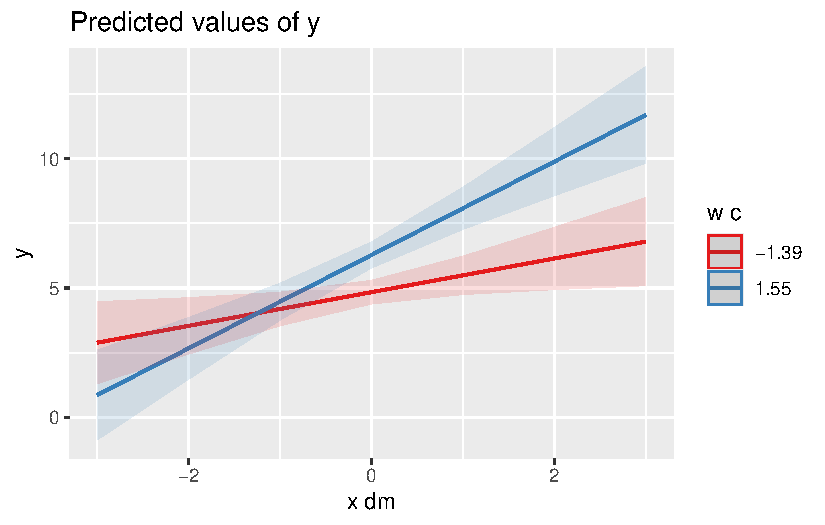
\includegraphics[keepaspectratio]{04-Hypotheses-Tests_Erweiterungen_files/figure-pdf/unnamed-chunk-6-1.pdf}}

Alternativ kann man auch die Werte zum Mittelwerte und bei -1 SD und +1
SD des Moderators anzeigen lassen. Wir können den zuletzt erzeugten Plot
mittels \texttt{ggsave()} abspeichern.

\begin{Shaded}
\begin{Highlighting}[]
\FunctionTok{plot\_model}\NormalTok{(ri.rs\_cli\_modell, }\AttributeTok{type =} \StringTok{"int"}\NormalTok{, }\AttributeTok{mdrt.values =} \StringTok{"meansd"}\NormalTok{)}
\end{Highlighting}
\end{Shaded}

\pandocbounded{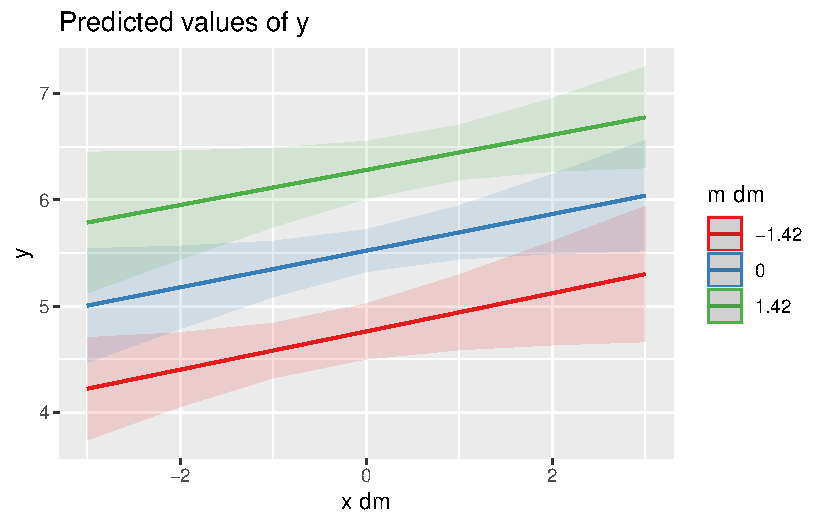
\includegraphics[keepaspectratio]{04-Hypotheses-Tests_Erweiterungen_files/figure-pdf/unnamed-chunk-7-1.pdf}}

\begin{Shaded}
\begin{Highlighting}[]
\FunctionTok{ggsave}\NormalTok{(}\StringTok{"Plots/CLI\_Beispiel.png"}\NormalTok{)}
\end{Highlighting}
\end{Shaded}

\begin{verbatim}
Saving 5.5 x 3.5 in image
\end{verbatim}

Der Plot zeigt, dass bei höheren Ausprägungen von w der Effekt von x\_dm
stärker ausfällt.

\subsection{Simple Slopes Analyse}\label{simple-slopes-analyse}

Mit Hilfe der \texttt{simple\_slopes()} Funktion aus dem
\texttt{reghelper} Paket können wir uns die Regressionskoeffizienten
einer Simple-Slope Analyse unterziehen. Die statistischen Kennwerte
dienen als Zusatz zur Visualisierung der Simple Slopes. So können wir
z.B. bestimmen, ob der Effekt von X auf Y auf verschiedenen Ausprägungen
signifikant ist. Z.B. könnte der Effekt von X auf Y nur bei bestimmten
Ausprägungen (hoch oder niedrig) signifikant sein.

Wir können die spezifischen Werte der Variable automatisch bestimmen (1.
Variante) oder manuell setzen (2. Variante). Uns interessieren die
Werte, wenn x\_dm um eine Einheit steigt und der Moderator
unterdurchschnittlich (-1 SD), durchschnittlich, oder
überdurchschnittlich (+1 SD) ist. Entsprechend werden die Werte in
Variante 2 manuell gesetzt. Die Werte können wir der Abbildung oben
entnehmen.

\begin{Shaded}
\begin{Highlighting}[]
\FunctionTok{simple\_slopes}\NormalTok{(ri.rs\_cli\_modell)}
\end{Highlighting}
\end{Shaded}

\begin{verbatim}
       x_dm       w_c Test Estimate Std. Error      df t value  Pr(>|t|) Sig.
1 -0.663149    sstest        0.2286     0.1800 96.6513  1.2699 0.2071831     
2         0    sstest        0.4892     0.1536 97.9998  3.1857 0.0019372   **
3  0.663149    sstest        0.7499     0.2049 97.1644  3.6598 0.0004104  ***
4    sstest -0.621309        0.9541     0.1554 95.4521  6.1399 1.884e-08  ***
5    sstest         0        1.1983     0.1100 95.8381 10.8934 < 2.2e-16  ***
6    sstest  0.621309        1.4424     0.1548 94.0928  9.3208 5.072e-15  ***
\end{verbatim}

\begin{Shaded}
\begin{Highlighting}[]
\FunctionTok{simple\_slopes}\NormalTok{(ri.rs\_cli\_modell,}
              \AttributeTok{levels =} \FunctionTok{list}\NormalTok{(}\AttributeTok{x\_dm =} \FunctionTok{c}\NormalTok{(}\DecValTok{1}\NormalTok{,}\StringTok{\textquotesingle{}sstest\textquotesingle{}}\NormalTok{) ),}
              \AttributeTok{w\_c =} \FunctionTok{c}\NormalTok{(}\SpecialCharTok{{-}}\FloatTok{0.62}\NormalTok{,}\DecValTok{0}\NormalTok{, }\FloatTok{0.62}\NormalTok{, }\StringTok{"sstest"}\NormalTok{))}
\end{Highlighting}
\end{Shaded}

\begin{verbatim}
    x_dm       w_c Test Estimate Std. Error      df t value  Pr(>|t|) Sig.
1      1    sstest        0.8823     0.2485 96.4987  3.5504 0.0005966  ***
2 sstest -0.621309        0.9541     0.1554 95.4521  6.1399 1.884e-08  ***
3 sstest         0        1.1983     0.1100 95.8381 10.8934 < 2.2e-16  ***
4 sstest  0.621309        1.4424     0.1548 94.0928  9.3208 5.072e-15  ***
\end{verbatim}

Die Simple Slope Analyse bestätigt die Visualiserung und zeigt, dass der
Effekt von x\_dm auf y schwächer ausfällt, aber immer noch signifikant
positiv ist, wenn der Moderator w\_c unterdurchschnittlich ist (Variante
1, Zeile 4; Variante 2, Zeile 2). Der Effekt fällt stärker aus, wenn der
Moderator w\_c überdurchschnittlich ist (Variante 1, Zeile 6; Variante
2, Zeile 4).

\subsection{Within-level Interaktion}\label{within-level-interaktion}

Analog zur Cross-level Interaktion gibt es auch Within-level
Interaktionen, bei der die Level-1 Anteile von Prädiktorvariablen
miteinander interagieren.

Level 1:
\(y_{ij} = \beta_{0j} + \beta_{1j}*(X_{ij}-\overline{X_j}) + \beta_{2j}*(M_{ij}-\overline{M_j}) + \beta_{3j}*((M_{ij}-\overline{M_j})*(X_{ij}-\overline{X_j})) + e_{ij}\)

Level 2 (random intercept): \(\beta_{0j} = \gamma_{00} + u_{0j}\)

Level 2 (random slope X): \(\beta_{1j} = \gamma_{10} + u_{1j}\)

Level 2 (random slope M): \(\beta_{2j} = \gamma_{20} + u_{2j}\)

\begin{Shaded}
\begin{Highlighting}[]
\NormalTok{ri.rs\_wli\_modell }\OtherTok{\textless{}{-}} \FunctionTok{lmer}\NormalTok{(y }\SpecialCharTok{\textasciitilde{}}\NormalTok{ x\_dm }\SpecialCharTok{+}\NormalTok{ m\_dm }\SpecialCharTok{+}\NormalTok{ x\_dm}\SpecialCharTok{*}\NormalTok{m\_dm }\SpecialCharTok{+}\NormalTok{ (}\DecValTok{1} \SpecialCharTok{+}\NormalTok{ x\_dm }\SpecialCharTok{+}\NormalTok{ m\_dm }\SpecialCharTok{|}\NormalTok{ id), }\AttributeTok{data =}\NormalTok{ df\_example1c)}
\FunctionTok{model\_parameters}\NormalTok{(ri.rs\_wli\_modell) }\SpecialCharTok{|\textgreater{}} \FunctionTok{print\_html}\NormalTok{()}
\end{Highlighting}
\end{Shaded}

\begingroup
\fontsize{12.0pt}{14.4pt}\selectfont
\setlength{\LTpost}{0mm}
\begin{longtable*}{lccccc}
\caption*{
{\large Model Summary}
} \\ 
\toprule
Parameter & Coefficient & SE & 95\% CI & t(989) & p \\ 
\midrule\addlinespace[2.5pt]
\multicolumn{6}{l}{Fixed Effects } \\[2.5pt] 
\midrule\addlinespace[2.5pt]
{(Intercept)} & 5.52 & 0.10 & (5.32, 5.72) & 54.89 & < .001 \\ 
{x dm} & 0.17 & 0.08 & (9.53e-03, 0.33) & 2.08 & 0.038  \\ 
{m dm} & 0.53 & 0.06 & (0.41, 0.66) & 8.46 & < .001 \\ 
{x dm × m dm} & -5.19e-03 & 0.02 & (-0.04, 0.02) & -0.34 & 0.735  \\ 
\midrule\addlinespace[2.5pt]
\multicolumn{6}{l}{Random Effects } \\[2.5pt] 
\midrule\addlinespace[2.5pt]
{SD (Intercept: id)} & 0.98 &  &  &  &  \\ 
{SD (x\_dm: id)} & 0.47 &  &  &  &  \\ 
{SD (m\_dm: id)} & 0.53 &  &  &  &  \\ 
{Cor (Intercept\textasciitilde{}x\_dm: id)} & -0.08 &  &  &  &  \\ 
{Cor (Intercept\textasciitilde{}m\_dm: id)} & 0.04 &  &  &  &  \\ 
{Cor (x\_dm\textasciitilde{}m\_dm: id)} & -0.26 &  &  &  &  \\ 
{SD (Residual)} & 0.52 &  &  &  &  \\ 
\bottomrule
\end{longtable*}
\begin{minipage}{\linewidth}
\\
\end{minipage}
\endgroup

\begin{Shaded}
\begin{Highlighting}[]
\FunctionTok{plot\_model}\NormalTok{(ri.rs\_wli\_modell, }\AttributeTok{type =} \StringTok{"int"}\NormalTok{, }\AttributeTok{mdrt.values =} \StringTok{"meansd"}\NormalTok{)}
\end{Highlighting}
\end{Shaded}

\pandocbounded{\includegraphics[keepaspectratio]{04-Hypotheses-Tests_Erweiterungen_files/figure-pdf/unnamed-chunk-10-1.pdf}}

Der Interaktionseffekt ist nicht signifikant. Dies bedeutet, wie der
Plot zeigt, dass die Linien bei allen Ausprägungen des Moderators mehr
oder wenig parallel sind.

\section{Übung}\label{uxfcbung-2}

Wir arbeiten in der Übung mit dem Übungs-Datensatz aus Kapitel 4.

\begin{Shaded}
\begin{Highlighting}[]
\FunctionTok{load}\NormalTok{(}\StringTok{"../data/df\_example\_cli.RData"}\NormalTok{)}

\FunctionTok{head}\NormalTok{(df\_example\_cli)}
\end{Highlighting}
\end{Shaded}

\begin{verbatim}
# A tibble: 6 x 10
     id illtask negativ support illtask_dm negativ_dm illtask_gm negativ_gm
  <int>   <dbl>   <dbl>   <dbl>      <dbl>      <dbl>      <dbl>      <dbl>
1     1    1.19    1.83    3.45    -1.30      -0.0154       2.49       1.84
2     1    1.72    1.63    3.45    -0.769     -0.208        2.49       1.84
3     1    3.15    1.25    3.45     0.661     -0.591        2.49       1.84
4     1    2.37    1.58    3.45    -0.116     -0.257        2.49       1.84
5     1    2.56    2.91    3.45     0.0702     1.07         2.49       1.84
6     2    1.34    2.11    2.11     0.281     -0.491        1.06       2.60
# i 2 more variables: negativ_dm_l1 <dbl>, day <int>
\end{verbatim}

\begin{Shaded}
\begin{Highlighting}[]
\FunctionTok{get\_label}\NormalTok{(df\_example\_cli)}
\end{Highlighting}
\end{Shaded}

\begin{verbatim}
                                         id 
                              "Personen-ID" 
                                    illtask 
                 "Daily Illegitimate Tasks" 
                                    negativ 
                    "Daily Negative Affect" 
                                    support 
                         "Coworker support" 
                                 illtask_dm 
"Illegitimate Tasks (person-mean centered)" 
                                 negativ_dm 
       "Neg. Affect (person-mean centered)" 
                                 illtask_gm 
      "Illegitimate Tasks (person average)" 
                                 negativ_gm 
             "Neg. Affect (person average)" 
                              negativ_dm_l1 
                 "Previous-day Neg. Affect" 
                                        day 
                               "Tag (1-10)" 
\end{verbatim}

\begin{Shaded}
\begin{Highlighting}[]
\CommentTok{\# alternativ}
\FunctionTok{view\_df}\NormalTok{(df\_example\_cli)}
\end{Highlighting}
\end{Shaded}

\begin{longtable}[]{@{}lllll@{}}
\caption{Data frame: df\_example\_cli}\tabularnewline
\toprule\noalign{}
\endfirsthead
\endhead
\bottomrule\noalign{}
\endlastfoot
ID & Name & Label & Values & Value Labels \\
1 & id & Personen-ID & \multicolumn{2}{l@{}}{%
\emph{range: 1-100}} \\
2 & illtask & Daily Illegitimate Tasks & \multicolumn{2}{l@{}}{%
\emph{range: -1.9-5.6}} \\
3 & negativ & Daily Negative Affect & \multicolumn{2}{l@{}}{%
\emph{range: -0.2-7.7}} \\
4 & support & Coworker support & \multicolumn{2}{l@{}}{%
\emph{range: 1.4-4.5}} \\
5 & illtask\_dm & Illegitimate Tasks (person-mean centered) &
\multicolumn{2}{l@{}}{%
\emph{range: -2.1-2.3}} \\
6 & negativ\_dm & Neg. Affect (person-mean centered) &
\multicolumn{2}{l@{}}{%
\emph{range: -2.0-2.7}} \\
7 & illtask\_gm & Illegitimate Tasks (person average) &
\multicolumn{2}{l@{}}{%
\emph{range: -0.7-4.7}} \\
8 & negativ\_gm & Neg. Affect (person average) & \multicolumn{2}{l@{}}{%
\emph{range: 0.8-5.0}} \\
9 & negativ\_dm\_l1 & Previous-day Neg. Affect & \multicolumn{2}{l@{}}{%
\emph{range: -2.0-2.7}} \\
10 & day & Tag (1-10) & \multicolumn{2}{l@{}}{%
\emph{range: 1-10}} \\
\end{longtable}

Berechne Modelle mit denen du die folgenden Hypothesen testest:

H1: Illegitime Aufgaben hängen positiv mit negativem Affekt zusammen.
H2: Der positive Zusammenhang von illegitime Aufgaben mit negativem
Affekt fällt schwächer aus, wenn Unterstützung von Kolleg:innen hoch
ausgeprägt ist.

Gehe Schritt für Schritt vor und teste erst in einem Modell H1 (verwende
dazu den Random Intercept, Random Slope Modell-Code aus dem letzten
Kapitel), dann in einem anderen Modell H2. Urteile, ob die Hypothesen
angenommen oder verworfen werden sollten.

\begin{tcolorbox}[enhanced jigsaw, opacitybacktitle=0.6, left=2mm, colback=white, rightrule=.15mm, title=\textcolor{quarto-callout-tip-color}{\faLightbulb}\hspace{0.5em}{Lösung}, breakable, leftrule=.75mm, colframe=quarto-callout-tip-color-frame, toptitle=1mm, toprule=.15mm, titlerule=0mm, arc=.35mm, bottomtitle=1mm, colbacktitle=quarto-callout-tip-color!10!white, coltitle=black, bottomrule=.15mm, opacityback=0]

\begin{Shaded}
\begin{Highlighting}[]
\NormalTok{ri.rs\_modell }\OtherTok{\textless{}{-}} \FunctionTok{lmer}\NormalTok{(negativ }\SpecialCharTok{\textasciitilde{}}\NormalTok{ illtask\_dm  }\SpecialCharTok{+}\NormalTok{ support }\SpecialCharTok{+}\NormalTok{ (}\DecValTok{1} \SpecialCharTok{+}\NormalTok{ illtask\_dm }\SpecialCharTok{|}\NormalTok{ id), }\AttributeTok{data =}\NormalTok{ df\_example\_cli)}
\FunctionTok{parameters}\NormalTok{(ri.rs\_modell)}
\end{Highlighting}
\end{Shaded}

\begin{verbatim}
# Fixed Effects

Parameter   | Coefficient |   SE |         95% CI | t(776) |      p
-------------------------------------------------------------------
(Intercept) |        3.45 | 0.30 | [ 2.86,  4.05] |  11.36 | < .001
illtask dm  |        0.33 | 0.05 | [ 0.22,  0.43] |   6.34 | < .001
support     |       -0.25 | 0.10 | [-0.45, -0.05] |  -2.44 | 0.015 

# Random Effects

Parameter                      | Coefficient
--------------------------------------------
SD (Intercept: id)             |        0.67
SD (illtask_dm: id)            |        0.35
Cor (Intercept~illtask_dm: id) |        0.69
SD (Residual)                  |        0.68
\end{verbatim}

\begin{verbatim}

Uncertainty intervals (equal-tailed) and p-values (two-tailed) computed
  using a Wald t-distribution approximation.
\end{verbatim}

Der Zusammenhang von täglichen illegitimen Aufgaben (illtask\_dm) mit
negativem Affekt (negativ) ist signifikant (b = 0.33, p \textless{}
.001), was Hypothese 1 unterstützt.

\begin{Shaded}
\begin{Highlighting}[]
\NormalTok{ri.rs\_cli\_modell }\OtherTok{\textless{}{-}} \FunctionTok{lmer}\NormalTok{(negativ }\SpecialCharTok{\textasciitilde{}}\NormalTok{ illtask\_dm  }\SpecialCharTok{+}\NormalTok{ support}\SpecialCharTok{*}\NormalTok{illtask\_dm }\SpecialCharTok{+}\NormalTok{ (}\DecValTok{1} \SpecialCharTok{+}\NormalTok{ illtask\_dm }\SpecialCharTok{|}\NormalTok{ id), }\AttributeTok{data =}\NormalTok{ df\_example\_cli)}
\FunctionTok{parameters}\NormalTok{(ri.rs\_cli\_modell)}
\end{Highlighting}
\end{Shaded}

\begin{verbatim}
# Fixed Effects

Parameter            | Coefficient |   SE |         95% CI | t(775) |      p
----------------------------------------------------------------------------
(Intercept)          |        3.47 | 0.34 | [ 2.81,  4.13] |  10.33 | < .001
illtask dm           |        0.36 | 0.25 | [-0.12,  0.84] |   1.46 | 0.144 
support              |       -0.25 | 0.11 | [-0.48, -0.03] |  -2.26 | 0.024 
illtask dm × support |       -0.01 | 0.08 | [-0.17,  0.15] |  -0.14 | 0.887 

# Random Effects

Parameter                      | Coefficient
--------------------------------------------
SD (Intercept: id)             |        0.67
SD (illtask_dm: id)            |        0.36
Cor (Intercept~illtask_dm: id) |        0.70
SD (Residual)                  |        0.68
\end{verbatim}

\begin{verbatim}

Uncertainty intervals (equal-tailed) and p-values (two-tailed) computed
  using a Wald t-distribution approximation.
\end{verbatim}

Der Interaktionseffekt von täglichen illegitimen Aufgaben mit sozialer
Unterstützung durch Kolleg:innen auf negativen Affekt ist nicht
signifikant (b = -0.01, p = .89). Hypothese 2 muss somit verworfen
werden.

\end{tcolorbox}

\section{1-1-1 Mediation}\label{mediation}

Die 1-1-1 Mediation ist die gängigste Variante, in der alle Variablen
(X, M{[}ediator{]}, und Y) auf Tagesebene gemessen werden.

\subsection{Daten einlesen}\label{daten-einlesen-2}

\begin{Shaded}
\begin{Highlighting}[]
\FunctionTok{load}\NormalTok{(}\StringTok{"../data/df\_example1.RData"}\NormalTok{)}
\FunctionTok{head}\NormalTok{(df\_example1)}
\end{Highlighting}
\end{Shaded}

\begin{verbatim}
# A tibble: 6 x 10
  id        y     m     x    y_dm   m_dm    x_dm  y_gm  m_gm  x_gm
  <fct> <dbl> <dbl> <dbl>   <dbl>  <dbl>   <dbl> <dbl> <dbl> <dbl>
1 1      4.00  4.77 2.37  -0.302   0.895  0.685   4.31  3.87  1.68
2 1      4.93  2.51 0.749  0.620  -1.36  -0.932   4.31  3.87  1.68
3 1      4.60  3.10 1.40   0.293  -0.777 -0.286   4.31  3.87  1.68
4 1      4.29  4.61 1.86  -0.0194  0.736  0.179   4.31  3.87  1.68
5 1      4.18  4.55 2.29  -0.122   0.674  0.607   4.31  3.87  1.68
6 1      3.63  3.59 1.70  -0.674  -0.285  0.0156  4.31  3.87  1.68
\end{verbatim}

Zum Testen des Mediationsmodells verwenden wir zunächst die Funktion
\texttt{modmed.mlm()}. Im Folgenden erstellen wir mit dieser Funktion
ein Mediationsmodell und spezifizieren bei den Argumenten X, Y, und M
die die unabhängige, abhängige, und mediierende Variable. Für die
abhängige Variable Y wählen wir die Rohvariable, für unabhängige und
mediierende Variablen die personen-zentrierten Variablen.

Anders als bei den früheren Analysen steht uns das \texttt{parameters}
Paket hier nicht zur Verfügung um die Ergebnisse zusammenzufassen.
Stattdessen nehmen wir die \texttt{summary()} Funktion oder die
\texttt{tidy()}-Funktion aus dem broom Paket.

\begin{Shaded}
\begin{Highlighting}[]
\NormalTok{fit\_mediation }\OtherTok{\textless{}{-}} \FunctionTok{modmed.mlm}\NormalTok{(}
\NormalTok{  df\_example1,}
  \AttributeTok{L2ID =} \StringTok{"id"}\NormalTok{,}
  \AttributeTok{X =} \StringTok{"x\_dm"}\NormalTok{,}
  \AttributeTok{Y =} \StringTok{"y"}\NormalTok{,}
  \AttributeTok{M =} \StringTok{"m\_dm"}\NormalTok{,}
  \AttributeTok{random.int.m =} \ConstantTok{FALSE}\NormalTok{,}
  \AttributeTok{na.action =}\NormalTok{ na.omit}
\NormalTok{)}

\CommentTok{\#summary(fit\_mediation$model)}
\NormalTok{broom}\SpecialCharTok{::}\FunctionTok{tidy}\NormalTok{(fit\_mediation}\SpecialCharTok{$}\NormalTok{model) }\SpecialCharTok{|\textgreater{}}
  \FunctionTok{mutate}\NormalTok{(}\FunctionTok{across}\NormalTok{(}\FunctionTok{where}\NormalTok{(is.numeric), round, }\DecValTok{2}\NormalTok{)) }\CommentTok{\# rundung der werte}
\end{Highlighting}
\end{Shaded}

\begin{verbatim}
Warning: There was 1 warning in `mutate()`.
i In argument: `across(where(is.numeric), round, 2)`.
Caused by warning:
! The `...` argument of `across()` is deprecated as of dplyr 1.1.0.
Supply arguments directly to `.fns` through an anonymous function instead.

  # Previously
  across(a:b, mean, na.rm = TRUE)

  # Now
  across(a:b, \(x) mean(x, na.rm = TRUE))
\end{verbatim}

\begin{verbatim}
# A tibble: 9 x 8
  effect    group            term     estimate std.error    df statistic p.value
  <chr>     <chr>            <chr>       <dbl>     <dbl> <dbl>     <dbl>   <dbl>
1 fixed     <NA>             Sm           0         0.02  1896      0          1
2 fixed     <NA>             Sy           5.37      0.09  1896     61.5        0
3 fixed     <NA>             SmX          0.51      0.03  1896     17.8        0
4 fixed     <NA>             SyX          0.14      0.04  1896      3.63       0
5 fixed     <NA>             SyM          0.58      0.04  1896     16.0        0
6 ran_pars  L2id             sd_Sy        0.84     NA       NA     NA         NA
7 ran_pars  Residual         sd_Obse~     0.7      NA       NA     NA         NA
8 var_model varIdent(1 | Sm) 0            1        NA       NA     NA         NA
9 var_model varIdent(1 | Sm) 1            0.87     NA       NA     NA         NA
\end{verbatim}

Die ausgegebenen Zeilen/Parameter sind etwas kryptisch beschrieben.

\begin{itemize}
\tightlist
\item
  Sm - fixed Intercept von M
\item
  Sy - fixed Intercept von Y
\item
  SmX - fixed Slope von X auf M (a-Pfad)
\item
  SyX - fixed Slope von Y auf X (c'-Pfad)
\item
  SyM - fixed Slope von Y auf M (b-Pfad)
\end{itemize}

\subsection{Bootstrapped Version}\label{bootstrapped-version}

Der indirekte Effekt von X auf Y via M (a-Pfad * b-Pfad) der uns in der
Mediation von zentralem Interesse ist, ist in der Regel nicht
normalverteilt, da ein Produkt zweier (oder mehrerer) Pfadkoeffizienten
nicht wie die Pfadkoeffizienten selber approximativ normalverteilt ist.
Aufgrund der fehlenden Normalverteilung verwenden wir die
Bootstrap-Schätzung, um eine robustere Aussage über die Signifikanz des
indirekten Effekts zu bekommen.

\begin{Shaded}
\begin{Highlighting}[]
\NormalTok{boot.custom.results }\OtherTok{\textless{}{-}} \FunctionTok{boot.modmed.mlm.custom}\NormalTok{(}
  \AttributeTok{data =}\NormalTok{ df\_example1 }\SpecialCharTok{|\textgreater{}} \FunctionTok{as.data.frame}\NormalTok{(),}
  \AttributeTok{L2ID =} \StringTok{"id"}\NormalTok{,}
  \AttributeTok{X =} \StringTok{"x\_dm"}\NormalTok{,}
  \AttributeTok{Y =} \StringTok{"y"}\NormalTok{,}
  \AttributeTok{M =} \StringTok{"m\_dm"}\NormalTok{,}
  \AttributeTok{random.int.m =} \ConstantTok{FALSE}\NormalTok{,}
  \AttributeTok{control =} \FunctionTok{list}\NormalTok{(}\AttributeTok{opt =} \StringTok{"nlm"}\NormalTok{),}
  \AttributeTok{na.action =}\NormalTok{ na.omit,}
  \AttributeTok{return.type =} \StringTok{"all"}\NormalTok{,}
  \AttributeTok{nrep =} \DecValTok{1000}\NormalTok{,}
  \AttributeTok{parallel.type =} \StringTok{"parallel"}\NormalTok{,}
  \AttributeTok{ncores =} \DecValTok{4}\NormalTok{,}
  \AttributeTok{seed =} \DecValTok{2299}\NormalTok{)}
\end{Highlighting}
\end{Shaded}

\begin{Shaded}
\begin{Highlighting}[]
\NormalTok{broom}\SpecialCharTok{::}\FunctionTok{tidy}\NormalTok{(boot.custom.results}\SpecialCharTok{$}\NormalTok{model) }\SpecialCharTok{|\textgreater{}}
  \FunctionTok{mutate}\NormalTok{(}\FunctionTok{across}\NormalTok{(}\FunctionTok{where}\NormalTok{(is.numeric), round, }\DecValTok{2}\NormalTok{)) }\CommentTok{\# rundung der werte}
\end{Highlighting}
\end{Shaded}

\begin{verbatim}
# A tibble: 9 x 8
  effect    group            term     estimate std.error    df statistic p.value
  <chr>     <chr>            <chr>       <dbl>     <dbl> <dbl>     <dbl>   <dbl>
1 fixed     <NA>             Sm           0         0.02  1896      0          1
2 fixed     <NA>             Sy           5.37      0.09  1896     61.5        0
3 fixed     <NA>             SmX          0.51      0.03  1896     17.8        0
4 fixed     <NA>             SyX          0.14      0.04  1896      3.63       0
5 fixed     <NA>             SyM          0.58      0.04  1896     16.0        0
6 ran_pars  L2id             sd_Sy        0.84     NA       NA     NA         NA
7 ran_pars  Residual         sd_Obse~     0.7      NA       NA     NA         NA
8 var_model varIdent(1 | Sm) 0            1        NA       NA     NA         NA
9 var_model varIdent(1 | Sm) 1            0.87     NA       NA     NA         NA
\end{verbatim}

Nach der Schätzung des Modells müssen wir das 95\% Konfidenzintervall
des indirekten Effekts aus den Modellergebnissen extrahieren. Dazu gibt
es derzeit keine einfache Funktion, entsprechend fällt der folgende
Code-Chunk komplexer aus.

\begin{Shaded}
\begin{Highlighting}[]
\CommentTok{\# Punktwert des indirekten Effekt}
\NormalTok{indirect\_punktschaetzung }\OtherTok{\textless{}{-}} \FunctionTok{extract.modmed.mlm}\NormalTok{(boot.custom.results, }\AttributeTok{type=}\StringTok{"indirect"}\NormalTok{)}

\CommentTok{\# Bootstrapped 95\% Konfidenzintervall um den Punktwert herum}
\NormalTok{indirect\_boot }\OtherTok{\textless{}{-}} \FunctionTok{tibble}\NormalTok{(}\AttributeTok{SyM =}\NormalTok{ boot.custom.results[[}\StringTok{"t"}\NormalTok{]][,}\FunctionTok{which}\NormalTok{(}\FunctionTok{names}\NormalTok{(boot.custom.results[[}\StringTok{"t0"}\NormalTok{]]) }\SpecialCharTok{==} \StringTok{"SyM"}\NormalTok{)], }
                        \AttributeTok{SmX =}\NormalTok{ boot.custom.results[[}\StringTok{"t"}\NormalTok{]][,}\FunctionTok{which}\NormalTok{(}\FunctionTok{names}\NormalTok{(boot.custom.results[[}\StringTok{"t0"}\NormalTok{]]) }\SpecialCharTok{==} \StringTok{"SmX"}\NormalTok{)]) }\SpecialCharTok{|\textgreater{}} 
  \FunctionTok{mutate}\NormalTok{(}\AttributeTok{indirect =}\NormalTok{ SyM }\SpecialCharTok{*}\NormalTok{ SmX)}
\NormalTok{indirekt\_ci }\OtherTok{\textless{}{-}} \FunctionTok{quantile}\NormalTok{(indirect\_boot}\SpecialCharTok{$}\NormalTok{indirect, }\FunctionTok{c}\NormalTok{(}\FloatTok{0.025}\NormalTok{, }\FloatTok{0.975}\NormalTok{), }\AttributeTok{na.rm =} \ConstantTok{TRUE}\NormalTok{)}

\CommentTok{\# zusammenfassen}
\NormalTok{indirekt\_zusammenfassung }\OtherTok{\textless{}{-}}
  \FunctionTok{tibble}\NormalTok{(}\AttributeTok{Koeffizient =}\NormalTok{ indirect\_punktschaetzung,}
         \AttributeTok{LLCI =}\NormalTok{ indirekt\_ci[}\DecValTok{1}\NormalTok{],}
         \AttributeTok{ULCI =}\NormalTok{ indirekt\_ci[}\DecValTok{2}\NormalTok{]) }\SpecialCharTok{|\textgreater{}} 
  \FunctionTok{mutate}\NormalTok{(}\FunctionTok{across}\NormalTok{(}\FunctionTok{where}\NormalTok{(is.numeric), round, }\DecValTok{3}\NormalTok{))}
\NormalTok{indirekt\_zusammenfassung}
\end{Highlighting}
\end{Shaded}

\begin{verbatim}
# A tibble: 1 x 3
  Koeffizient  LLCI  ULCI
        <dbl> <dbl> <dbl>
1         0.3 0.198 0.411
\end{verbatim}

\begin{itemize}
\tightlist
\item
  LLCI = Lower Limit of Confidence Interval
\item
  ULCI = Upper Limit of Confidence Interval
\end{itemize}

Der indirekte Effekt und sein 95\% Konfidenzintervall müssen wir aus den
Daten extrahieren. Wenn der 95\% Konfidenzintervall die 0 ausschliesst
(also sowohl unterer als auch oberes Limit entweder unter Null oder über
Null liegen) können wir den indirekten Effekt als signifikant ansehen.

In diesem Beispiel finden wir also einen signifikanten indirekten Effekt
mit Koeffizient = 0.30, 95\% CI = {[}0.19, 0.41{]}.

\section{Übung}\label{uxfcbung-3}

Wir arbeiten in der Übung mit einem neuen Datensatz.

Mache dich mit ihm vertraut. Wie in der Cross-Level Interaktionsübung
benutzen wir einen Datensatz in dem die Variablen ``labelled'' sind,
also Beschriftungen haben. Wir können die Labels mit
\texttt{get\_label()} abrufen.

\begin{Shaded}
\begin{Highlighting}[]
\FunctionTok{load}\NormalTok{(}\StringTok{"../data/df\_111\_uebung.RData"}\NormalTok{)}

\FunctionTok{head}\NormalTok{(df\_111\_uebung)}
\end{Highlighting}
\end{Shaded}

\begin{verbatim}
# A tibble: 6 x 8
  id    helfen wertschaetz selbstwert wertschaetz_dm selbstwert_dm
  <fct>  <dbl>       <dbl>      <dbl>          <dbl>         <dbl>
1 1       4.71       1.37        4.44        -0.0438        -0.706
2 1       3.62       0.574       5.98        -0.841          0.835
3 1       5.34       1.47        5.41         0.0566         0.260
4 1       4.94       2.79        5.43         1.37           0.282
5 1       3.74       1.20        5.37        -0.211          0.223
6 1       4.61       1.74        4.64         0.329         -0.503
# i 2 more variables: wertschaetz_gm <dbl>, selbstwert_gm <dbl>
\end{verbatim}

\begin{Shaded}
\begin{Highlighting}[]
\FunctionTok{get\_label}\NormalTok{(df\_111\_uebung)}
\end{Highlighting}
\end{Shaded}

\begin{verbatim}
                                               id 
                                    "Personen-ID" 
                                           helfen 
                              "Proaktives Helfen" 
                                      wertschaetz 
                       "erfahrene Wertschaetzung" 
                                       selbstwert 
                                     "Selbstwert" 
                                   wertschaetz_dm 
"erfahrene Wertschaetzung (person-mean centered)" 
                                    selbstwert_dm 
              "Selbstwert (person-mean centered)" 
                                   wertschaetz_gm 
      "erfahrene Wertschaetzung (person average)" 
                                    selbstwert_gm 
                    "Selbstwert (person average)" 
\end{verbatim}

\begin{Shaded}
\begin{Highlighting}[]
\CommentTok{\# alternativ}
\FunctionTok{view\_df}\NormalTok{(df\_111\_uebung)}
\end{Highlighting}
\end{Shaded}

\begin{longtable}[]{@{}
  >{\raggedright\arraybackslash}p{(\linewidth - 8\tabcolsep) * \real{0.2000}}
  >{\raggedright\arraybackslash}p{(\linewidth - 8\tabcolsep) * \real{0.2000}}
  >{\raggedright\arraybackslash}p{(\linewidth - 8\tabcolsep) * \real{0.2000}}
  >{\raggedright\arraybackslash}p{(\linewidth - 8\tabcolsep) * \real{0.2000}}
  >{\raggedright\arraybackslash}p{(\linewidth - 8\tabcolsep) * \real{0.2000}}@{}}
\caption{Data frame: df\_111\_uebung}\tabularnewline
\toprule\noalign{}
\endfirsthead
\endhead
\bottomrule\noalign{}
\endlastfoot
ID & Name & Label & Values & Value Labels \\
1 & id & Personen-ID & & \begin{minipage}[t]{\linewidth}\raggedright
1\\
2\\
3\\
4\\
5\\
6\\
7\\
8\\
9\\
10\\
11\\
12\\
13\\
14\\
15\\
{\textless... truncated\textgreater{}}\strut
\end{minipage} \\
2 & helfen & Proaktives Helfen &
\multicolumn{2}{>{\raggedright\arraybackslash}p{(\linewidth - 8\tabcolsep) * \real{0.4000} + 2\tabcolsep}@{}}{%
\emph{range: 0.1-9.1}} \\
3 & wertschaetz & erfahrene Wertschaetzung &
\multicolumn{2}{>{\raggedright\arraybackslash}p{(\linewidth - 8\tabcolsep) * \real{0.4000} + 2\tabcolsep}@{}}{%
\emph{range: -2.4-5.5}} \\
4 & selbstwert & Selbstwert &
\multicolumn{2}{>{\raggedright\arraybackslash}p{(\linewidth - 8\tabcolsep) * \real{0.4000} + 2\tabcolsep}@{}}{%
\emph{range: 0.9-8.0}} \\
5 & wertschaetz\_dm & erfahrene Wertschaetzung (person-mean centered) &
\multicolumn{2}{>{\raggedright\arraybackslash}p{(\linewidth - 8\tabcolsep) * \real{0.4000} + 2\tabcolsep}@{}}{%
\emph{range: -2.0-2.4}} \\
6 & selbstwert\_dm & Selbstwert (person-mean centered) &
\multicolumn{2}{>{\raggedright\arraybackslash}p{(\linewidth - 8\tabcolsep) * \real{0.4000} + 2\tabcolsep}@{}}{%
\emph{range: -2.7-2.5}} \\
7 & wertschaetz\_gm & erfahrene Wertschaetzung (person average) &
\multicolumn{2}{>{\raggedright\arraybackslash}p{(\linewidth - 8\tabcolsep) * \real{0.4000} + 2\tabcolsep}@{}}{%
\emph{range: -1.0-4.6}} \\
8 & selbstwert\_gm & Selbstwert (person average) &
\multicolumn{2}{>{\raggedright\arraybackslash}p{(\linewidth - 8\tabcolsep) * \real{0.4000} + 2\tabcolsep}@{}}{%
\emph{range: 2.7-6.4}} \\
\end{longtable}

Berechne Modelle mit denen du die folgenden Hypothesen testest:

H1: Tägliche Wertschätzung durch Vorgesetzte und Kolleg:innen hängen
positiv mit dem täglichen Selbstwert zusammen. H2: Täglicher Selbstwert
hängt positiv mit täglichem proaktivem Helfen zusammen. H3: Es gibt
einen positiven indirekten Zusammenhang zwischen täglicher Wertschätzung
und täglichem proaktiven Helfen, vermittel durch den täglichen
Selbstwert.

Teste die Hypothesen in einem Modell mittels der
\texttt{boot.modmed.mlm.custom()} Funktion. Urteile, ob die Hypothesen
angenommen oder verworfen werden sollten.

\begin{tcolorbox}[enhanced jigsaw, opacitybacktitle=0.6, left=2mm, colback=white, rightrule=.15mm, title=\textcolor{quarto-callout-tip-color}{\faLightbulb}\hspace{0.5em}{Lösung}, breakable, leftrule=.75mm, colframe=quarto-callout-tip-color-frame, toptitle=1mm, toprule=.15mm, titlerule=0mm, arc=.35mm, bottomtitle=1mm, colbacktitle=quarto-callout-tip-color!10!white, coltitle=black, bottomrule=.15mm, opacityback=0]

\begin{Shaded}
\begin{Highlighting}[]
\CommentTok{\# | cache: true}
\NormalTok{boot.custom.results }\OtherTok{\textless{}{-}} \FunctionTok{boot.modmed.mlm.custom}\NormalTok{(}
  \AttributeTok{data =}\NormalTok{ df\_111\_uebung }\SpecialCharTok{|\textgreater{}} \FunctionTok{remove\_all\_labels}\NormalTok{(),}
  \AttributeTok{L2ID =} \StringTok{"id"}\NormalTok{,}
  \AttributeTok{X =} \StringTok{"wertschaetz\_dm"}\NormalTok{,}
  \AttributeTok{Y =} \StringTok{"helfen"}\NormalTok{,}
  \AttributeTok{M =} \StringTok{"selbstwert\_dm"}\NormalTok{,}
  \AttributeTok{random.int.m =} \ConstantTok{FALSE}\NormalTok{,}
  \AttributeTok{control =} \FunctionTok{list}\NormalTok{(}\AttributeTok{opt =} \StringTok{"nlm"}\NormalTok{),}
  \AttributeTok{na.action =}\NormalTok{ na.omit,}
  \AttributeTok{return.type =} \StringTok{"all"}\NormalTok{,}
  \AttributeTok{nrep =} \DecValTok{1000}\NormalTok{,}
  \AttributeTok{parallel.type =} \StringTok{"parallel"}\NormalTok{,}
  \AttributeTok{ncores =} \DecValTok{4}\NormalTok{,}
  \AttributeTok{seed =} \DecValTok{2299}\NormalTok{)}
\end{Highlighting}
\end{Shaded}

\begin{Shaded}
\begin{Highlighting}[]
\NormalTok{broom}\SpecialCharTok{::}\FunctionTok{tidy}\NormalTok{(boot.custom.results}\SpecialCharTok{$}\NormalTok{model) }\SpecialCharTok{|\textgreater{}}
  \FunctionTok{mutate}\NormalTok{(}\FunctionTok{across}\NormalTok{(}\FunctionTok{where}\NormalTok{(is.numeric), round, }\DecValTok{2}\NormalTok{)) }\CommentTok{\# rundung der werte}
\end{Highlighting}
\end{Shaded}

\begin{verbatim}
# A tibble: 9 x 8
  effect    group            term     estimate std.error    df statistic p.value
  <chr>     <chr>            <chr>       <dbl>     <dbl> <dbl>     <dbl>   <dbl>
1 fixed     <NA>             Sm           0         0.02  1896      0          1
2 fixed     <NA>             Sy           4.76      0.1   1896     49.4        0
3 fixed     <NA>             SmX          0.4       0.03  1896     13.8        0
4 fixed     <NA>             SyX          0.33      0.04  1896      8.93       0
5 fixed     <NA>             SyM          0.14      0.04  1896      3.84       0
6 ran_pars  L2id             sd_Sy        0.94     NA       NA     NA         NA
7 ran_pars  Residual         sd_Obse~     0.74     NA       NA     NA         NA
8 var_model varIdent(1 | Sm) 0            1        NA       NA     NA         NA
9 var_model varIdent(1 | Sm) 1            0.85     NA       NA     NA         NA
\end{verbatim}

\begin{Shaded}
\begin{Highlighting}[]
\CommentTok{\# Punktwert des indirekten Effekt}
\NormalTok{indirect\_punktschaetzung }\OtherTok{\textless{}{-}} \FunctionTok{extract.modmed.mlm}\NormalTok{(boot.custom.results, }\AttributeTok{type=}\StringTok{"indirect"}\NormalTok{)}

\CommentTok{\# Bootstrapped 95\% Konfidenzintervall um den Punktwert herum}
\NormalTok{indirect\_boot }\OtherTok{\textless{}{-}} \FunctionTok{tibble}\NormalTok{(}\AttributeTok{SyM =}\NormalTok{ boot.custom.results[[}\StringTok{"t"}\NormalTok{]][,}\FunctionTok{which}\NormalTok{(}\FunctionTok{names}\NormalTok{(boot.custom.results[[}\StringTok{"t0"}\NormalTok{]]) }\SpecialCharTok{==} \StringTok{"SyM"}\NormalTok{)], }
                        \AttributeTok{SmX =}\NormalTok{ boot.custom.results[[}\StringTok{"t"}\NormalTok{]][,}\FunctionTok{which}\NormalTok{(}\FunctionTok{names}\NormalTok{(boot.custom.results[[}\StringTok{"t0"}\NormalTok{]]) }\SpecialCharTok{==} \StringTok{"SmX"}\NormalTok{)]) }\SpecialCharTok{|\textgreater{}} 
  \FunctionTok{mutate}\NormalTok{(}\AttributeTok{indirect =}\NormalTok{ SyM }\SpecialCharTok{*}\NormalTok{ SmX)}
\NormalTok{indirekt\_ci }\OtherTok{\textless{}{-}} \FunctionTok{quantile}\NormalTok{(indirect\_boot}\SpecialCharTok{$}\NormalTok{indirect, }\FunctionTok{c}\NormalTok{(}\FloatTok{0.025}\NormalTok{, }\FloatTok{0.975}\NormalTok{), }\AttributeTok{na.rm =} \ConstantTok{TRUE}\NormalTok{)}

\CommentTok{\# zusammenfassen}
\NormalTok{indirekt\_zusammenfassung }\OtherTok{\textless{}{-}}
  \FunctionTok{tibble}\NormalTok{(}\AttributeTok{Koeffizient =}\NormalTok{ indirect\_punktschaetzung,}
         \AttributeTok{LLCI =}\NormalTok{ indirekt\_ci[}\DecValTok{1}\NormalTok{],}
         \AttributeTok{ULCI =}\NormalTok{ indirekt\_ci[}\DecValTok{2}\NormalTok{]) }\SpecialCharTok{|\textgreater{}} 
  \FunctionTok{mutate}\NormalTok{(}\FunctionTok{across}\NormalTok{(}\FunctionTok{where}\NormalTok{(is.numeric), round, }\DecValTok{3}\NormalTok{))}
\NormalTok{indirekt\_zusammenfassung}
\end{Highlighting}
\end{Shaded}

\begin{verbatim}
# A tibble: 1 x 3
  Koeffizient   LLCI  ULCI
        <dbl>  <dbl> <dbl>
1       0.057 -0.005 0.138
\end{verbatim}

H1 wird unterstützt (SmX: b = 0.40, \emph{p} \textless{} .001). H2 wird
verworfen (SyM: b = 0.14, \emph{p} \textless{} .40). H3: wird
entsprechend auch verworfen (95\% CI des indirekten Effekt schliesst die
0 ein). Es besteht aber ein direkter Zusammenhang zwischen X und Y (SyX:
b = 0.33, \emph{p} \textless{} .001), der, anders als angenommen, nicht
indirekt über Selbstwert vermittelt wird.

\end{tcolorbox}

\bookmarksetup{startatroot}

\chapter{Anhang: Data Wrangling}\label{anhang-data-wrangling}

Data Wrangling bezeichnet im Kontext der psychologischen Datenanalyse
mit R den systematischen Prozess der Aufbereitung, Bereinigung und
Umstrukturierung von Rohdaten, damit sie für statistische Auswertungen
und Interpretationen nutzbar werden. Ziel ist es, aus unübersichtlichen
Rohdaten ein strukturiertes und hochwertiges Daten-Set zu erzeugen, das
sich zuverlässig und nachvollziehbar für weiterführende statistische
Analysen, Modellierungen und Visualisierungen in R nutzen lässt.

Im Folgenden werden dazu verschiedene Funktionen und Techniken
dargestellt.

\begin{itemize}
\tightlist
\item
  basierend auf
  \href{https://github.com/ianhussey/data-wrangling-workshop/}{Kurs von
  Ian Hussey}
\item
  Siehe auch
  \href{https://methodenlehre.github.io/einfuehrung-in-R/}{Einführung in
  R}
\end{itemize}

\section{Notebooks}\label{notebooks}

In diesem Kurs arbeiten wir mit R- bzw. Quarto-Notebooks. Diese
enthalten sowohl normalen Text als auch ``Chunks'' von R-Code. Chunks
sind Abschnitte von R-Code. Diese Chunks lassen sich mit einem Klick auf
Code --\textgreater{} Insert Chunk (oder der Tastenkombination Alt +
Ctrl + I / unter Mac: Alt + Cmd + I) einfügen. Diese Chunks lassen sich
mit einem Klick auf den grünen Play-Button ganz rechts ausführen. Der
Pfeil nach unten Button (zweiter von Rechts) führt alle Chunks, die vor
dem gewählten Chunk gelagert sind, aus.

\section{Pakete laden}\label{pakete-laden-1}

Zunächst laden wir die Pakete, die wir für die Sitzung brauchen.

\begin{Shaded}
\begin{Highlighting}[]
\ControlFlowTok{if}\NormalTok{ (}\SpecialCharTok{!}\FunctionTok{require}\NormalTok{(}\StringTok{"pacman"}\NormalTok{)) }\FunctionTok{install.packages}\NormalTok{(}\StringTok{"pacman"}\NormalTok{)}
\end{Highlighting}
\end{Shaded}

\begin{verbatim}
Lade nötiges Paket: pacman
\end{verbatim}

\begin{Shaded}
\begin{Highlighting}[]
\NormalTok{pacman}\SpecialCharTok{::}\FunctionTok{p\_load}\NormalTok{(psych, tidyverse)}
\FunctionTok{data}\NormalTok{(sat.act)}
\NormalTok{df\_beispiel }\OtherTok{\textless{}{-}}\FunctionTok{as\_tibble}\NormalTok{(sat.act)}
\end{Highlighting}
\end{Shaded}

\section{Hilfe-Menü und
Dokumentation}\label{hilfe-menuxfc-und-dokumentation}

Für jede Funktion in einem geladenen Paket können Sie einfach \texttt{?}
vor den Funktionsnamen schreiben, um das Hilfemenü bzw. ihre
Dokumentation aufzurufen. Dies hilft Ihnen, den Zweck der Funktion, ihre
Argumente und Ausgaben zu verstehen. Sie können auch auf den Namen der
Funktion klicken (an beliebiger Stelle im Namen) und ``F1'' drücken.

\begin{Shaded}
\begin{Highlighting}[]
\NormalTok{?head}
\FunctionTok{head}\NormalTok{(df\_beispiel)}
\end{Highlighting}
\end{Shaded}

\section{Struktur von Funktionen}\label{struktur-von-funktionen}

Fast alles in R geschieht mittels Funktionen. Funktionen nehmen Inputs
und transformieren sie nach den Regeln der Funktion in Outputs. Die
Funktion kann mittels Argumenten gesteuert werden.

\begin{itemize}
\tightlist
\item
  Funktionen sind i.d.R. benannt (hier \texttt{head}, \texttt{mean}) und
  mit Klammern \texttt{()} gekennzeichet. In der Klammer befinden sich
  die Argumente der Funktion, mit einem Komma getrennt. Argumente können
  benannt oder unbenannt sein. Werden Sie nicht benannt, folgt R der
  Reihenfolge der erwarteten Argumente, wie sie in der
  Funktionsdokumentation beschrieben sind.
\item
  Unbenannt hier: \texttt{10} bei head()
\item
  Benannt hier: \texttt{na.rm\ =\ TRUE} bei mean(), wobei na.rm der Name
  und TRUE der Inhalt des Argument sind.
\end{itemize}

\begin{Shaded}
\begin{Highlighting}[]
\FunctionTok{head}\NormalTok{(df\_beispiel, }\DecValTok{10}\NormalTok{)}
\end{Highlighting}
\end{Shaded}

\begin{verbatim}
# A tibble: 10 x 6
   gender education   age   ACT  SATV  SATQ
    <int>     <int> <int> <int> <int> <int>
 1      2         3    19    24   500   500
 2      2         3    23    35   600   500
 3      2         3    20    21   480   470
 4      1         4    27    26   550   520
 5      1         2    33    31   600   550
 6      1         5    26    28   640   640
 7      2         5    30    36   610   500
 8      1         3    19    22   520   560
 9      2         4    23    22   400   600
10      2         5    40    35   730   800
\end{verbatim}

\begin{Shaded}
\begin{Highlighting}[]
\FunctionTok{mean}\NormalTok{(df\_beispiel}\SpecialCharTok{$}\NormalTok{age, }\AttributeTok{na.rm =} \ConstantTok{TRUE}\NormalTok{)}
\end{Highlighting}
\end{Shaded}

\begin{verbatim}
[1] 25.59429
\end{verbatim}

\section{Zuweisung / Assignment mittels
\textless-}\label{zuweisung-assignment-mittels--}

\begin{itemize}
\tightlist
\item
  \texttt{\textless{}-} führt die Zuweisung (assignment) von Inhalten
  der rechten Seite unter dem Namen auf der linken Seite aus. Wir nennen
  die zugewiesenen Inhalte, etwas verkürzt gesagt, Objekte oder
  Variablen.
\end{itemize}

\begin{Shaded}
\begin{Highlighting}[]
\NormalTok{durchschnitt\_von\_SATV }\OtherTok{\textless{}{-}} \FunctionTok{mean}\NormalTok{(df\_beispiel}\SpecialCharTok{$}\NormalTok{SATV, }\AttributeTok{na.rm =} \ConstantTok{TRUE}\NormalTok{)}
\end{Highlighting}
\end{Shaded}

In diesem Beispiel ist durchschnitt\_von\_SATV der Name des
Objekts/Variable.

\section{Typen von Objekten}\label{typen-von-objekten}

Die häufigsten Typen von Objekten/Variablen sind:

\begin{itemize}
\tightlist
\item
  Vektor, numerisch
\item
  Vektor, Character (Buchstaben)
\item
  data frame (Datenframe, Tabelle)
\item
  tibble - eine verbesserte Variante eines data frame
\item
  list (Liste)
\end{itemize}

Einen Vektor erstellt man mit der \texttt{c()} Funktionen

\begin{Shaded}
\begin{Highlighting}[]
\NormalTok{vektor\_numerisch }\OtherTok{\textless{}{-}} \FunctionTok{c}\NormalTok{(}\DecValTok{1}\NormalTok{,}\DecValTok{2}\NormalTok{,}\DecValTok{3}\NormalTok{,}\DecValTok{4}\NormalTok{,}\DecValTok{5}\NormalTok{)}
\NormalTok{vektor\_character }\OtherTok{\textless{}{-}} \FunctionTok{c}\NormalTok{(}\StringTok{"Zytglogge"}\NormalTok{, }\StringTok{"Hirschengraben"}\NormalTok{, }\StringTok{"Bahnhof"}\NormalTok{, }\StringTok{"Bundesplatz"}\NormalTok{, }\StringTok{"Viktoriaplatz"}\NormalTok{)}
\NormalTok{datenframe }\OtherTok{\textless{}{-}} \FunctionTok{data.frame}\NormalTok{(}\AttributeTok{Nummer =}\NormalTok{ vektor\_numerisch, }\AttributeTok{Ort =}\NormalTok{ vektor\_character)}
\NormalTok{datenframe}
\end{Highlighting}
\end{Shaded}

\begin{verbatim}
  Nummer            Ort
1      1      Zytglogge
2      2 Hirschengraben
3      3        Bahnhof
4      4    Bundesplatz
5      5  Viktoriaplatz
\end{verbatim}

\begin{Shaded}
\begin{Highlighting}[]
\NormalTok{tibble\_beispiel }\OtherTok{\textless{}{-}} \FunctionTok{tibble}\NormalTok{(}\AttributeTok{Nummer =}\NormalTok{ vektor\_numerisch, }\AttributeTok{Ort =}\NormalTok{ vektor\_character)}
\NormalTok{tibble\_beispiel}
\end{Highlighting}
\end{Shaded}

\begin{verbatim}
# A tibble: 5 x 2
  Nummer Ort           
   <dbl> <chr>         
1      1 Zytglogge     
2      2 Hirschengraben
3      3 Bahnhof       
4      4 Bundesplatz   
5      5 Viktoriaplatz 
\end{verbatim}

Wie wir sehen, sind Datenframes i.d.R. aus Vektoren der gleichen Länge,
aber oft unterschiedlichen Typs, aufgebaut.

\begin{Shaded}
\begin{Highlighting}[]
\NormalTok{beispielliste }\OtherTok{\textless{}{-}} \FunctionTok{list}\NormalTok{(}\AttributeTok{x1 =}\NormalTok{ vektor\_numerisch, }\AttributeTok{x2 =}\NormalTok{ vektor\_character, }\FunctionTok{c}\NormalTok{(}\DecValTok{6}\NormalTok{,}\DecValTok{7}\NormalTok{,}\DecValTok{8}\NormalTok{), }\AttributeTok{x3 =}\NormalTok{ tibble\_beispiel, }\StringTok{"test"}\NormalTok{)}
\NormalTok{beispielliste}
\end{Highlighting}
\end{Shaded}

\begin{verbatim}
$x1
[1] 1 2 3 4 5

$x2
[1] "Zytglogge"      "Hirschengraben" "Bahnhof"        "Bundesplatz"   
[5] "Viktoriaplatz" 

[[3]]
[1] 6 7 8

$x3
# A tibble: 5 x 2
  Nummer Ort           
   <dbl> <chr>         
1      1 Zytglogge     
2      2 Hirschengraben
3      3 Bahnhof       
4      4 Bundesplatz   
5      5 Viktoriaplatz 

[[5]]
[1] "test"
\end{verbatim}

Listen sind extrem flexibel, was ihre Anhalte angeht - wir können quasi
alles reinpacken. Das macht sie teils aber auch schwer zu durchschauen.
Wenn möglich empfiehlt es sich, mit tibble/data.frame zu arbeiten; dies
spart kognitive Ressourcen.

\section{Die ``Pipe'' (\%\textgreater\% oder
\textbar\textgreater)}\label{die-pipe-oder}

\texttt{\%\textgreater{}\%} ist der ursprüngliche Pipe-Operator, der für
das Paket \{magrittr\} entwickelt wurde und in den gesamten
tidyverse-Paketen verwendet wird. Er ist etwas langsamer, aber auch
flexibler. \texttt{\textbar{}\textgreater{}} ist eine neuere Version des
Pipe-Operators, die in Base-R integriert wurde. Sie ist etwas schneller,
aber weniger flexibel.

Die Ausgabe des linken Teils der Pipe wird als Eingabe für den rechten
Teil der Pipe verwendet, in der Regel als erstes Argument oder als
Datenargument. Effektiv transportiert die Pipe den Inhalt von links nach
rechts weiter. Schreiben lässt sich die Pipe mit den Tasten Ctrl + Shift
+ M (unter Windows; unter Mac Cmd + Shift + M?).

\begin{Shaded}
\begin{Highlighting}[]
\CommentTok{\# use a function without the pipe}
\NormalTok{example\_without\_pipe }\OtherTok{\textless{}{-}} \FunctionTok{select}\NormalTok{(df\_beispiel, gender, ACT)}

\CommentTok{\# use a function with the pipe. }
\NormalTok{example\_with\_pipe }\OtherTok{\textless{}{-}}\NormalTok{ df\_beispiel }\SpecialCharTok{|\textgreater{}} 
  \FunctionTok{select}\NormalTok{(gender, ACT)}


\NormalTok{example\_without\_pipe}
\end{Highlighting}
\end{Shaded}

\begin{verbatim}
# A tibble: 700 x 2
   gender   ACT
    <int> <int>
 1      2    24
 2      2    35
 3      2    21
 4      1    26
 5      1    31
 6      1    28
 7      2    36
 8      1    22
 9      2    22
10      2    35
# i 690 more rows
\end{verbatim}

\begin{Shaded}
\begin{Highlighting}[]
\NormalTok{example\_with\_pipe}
\end{Highlighting}
\end{Shaded}

\begin{verbatim}
# A tibble: 700 x 2
   gender   ACT
    <int> <int>
 1      2    24
 2      2    35
 3      2    21
 4      1    26
 5      1    31
 6      1    28
 7      2    36
 8      1    22
 9      2    22
10      2    35
# i 690 more rows
\end{verbatim}

\begin{Shaded}
\begin{Highlighting}[]
\CommentTok{\# check they produce identical results}
\FunctionTok{identical}\NormalTok{(example\_without\_pipe, example\_with\_pipe)}
\end{Highlighting}
\end{Shaded}

\begin{verbatim}
[1] TRUE
\end{verbatim}

\subsection{Warum lohnt es sich, die Pipe zu
nutzen?}\label{warum-lohnt-es-sich-die-pipe-zu-nutzen}

Der Pipe-Operator ermöglicht es uns, Code zu schreiben, der von oben
nach unten gelesen wird und einer Abfolge von Schritten folgt -- so, wie
Menschen Schritte organisieren und beschreiben. Ohne den Pipe-Operator
wird der Code von innen nach aussen geschrieben, auf eine Weise, die der
Computer versteht, aber für Menschen weniger intuitiv ist. Die
Unterscheide in der Lesbarkeit zeigen sich vor allem bei komplexeren,
verketteten Funktionen.

Wir verwenden im Folgenden einen Datenframe, wählen mit select() Spalten
aus, und erstellen ihre Mittelwerte mit colMeans(). Ohne Pipe lesen wir
von innen nach aussen: select(\ldots), dann colMeans(\ldots); mit Pipe
lesen und schreiben wir: Objekt - select() - colMeans(), was einfacher
nachzuvollziehen ist. Jede Funktion macht etwas, die Pipe gibt jeweils
den transformierten Inhalt weiter an die nächste Funktion.

\begin{Shaded}
\begin{Highlighting}[]
\CommentTok{\# use a function without the pipe}
\NormalTok{example\_without\_pipe }\OtherTok{\textless{}{-}} \FunctionTok{colMeans}\NormalTok{(}\FunctionTok{select}\NormalTok{(df\_beispiel, SATV, SATQ), }\AttributeTok{na.rm =} \ConstantTok{TRUE}\NormalTok{)}

\NormalTok{example\_without\_pipe}
\end{Highlighting}
\end{Shaded}

\begin{verbatim}
    SATV     SATQ 
612.2343 610.2169 
\end{verbatim}

\begin{Shaded}
\begin{Highlighting}[]
\CommentTok{\# use a function with the pipe. }
\NormalTok{example\_with\_pipe }\OtherTok{\textless{}{-}}\NormalTok{ df\_beispiel }\SpecialCharTok{|\textgreater{}} 
  \FunctionTok{select}\NormalTok{(SATV, SATQ) }\SpecialCharTok{|\textgreater{}} 
  \FunctionTok{colMeans}\NormalTok{(}\AttributeTok{na.rm =} \ConstantTok{TRUE}\NormalTok{)}

\CommentTok{\# check they produce identical results}
\FunctionTok{identical}\NormalTok{(example\_without\_pipe, example\_with\_pipe)}
\end{Highlighting}
\end{Shaded}

\begin{verbatim}
[1] TRUE
\end{verbatim}

\section{Spaltennamen anzeigen}\label{spaltennamen-anzeigen}

Die meiste Zeit verbringen wir mit Data Frames - effektiv Tabellen. Wie
können wir herausfinden, welche Variablen sich in einem Data Frame
befinden? Wir können den Data Frame anzeigen, aber es kann auch
hilfreich sein, ihn auszugeben. Zu wissen, welche Variablen vorhanden
sind, ist einer der ersten Schritte, um mit den Daten zu arbeiten.

\begin{Shaded}
\begin{Highlighting}[]
\CommentTok{\# print all column names}
\FunctionTok{colnames}\NormalTok{(df\_beispiel)}
\end{Highlighting}
\end{Shaded}

\begin{verbatim}
[1] "gender"    "education" "age"       "ACT"       "SATV"      "SATQ"     
\end{verbatim}

\begin{Shaded}
\begin{Highlighting}[]
\CommentTok{\# print all column names as a vector using the pipe}
\NormalTok{df\_beispiel }\SpecialCharTok{|\textgreater{}} 
  \FunctionTok{colnames}\NormalTok{()}
\end{Highlighting}
\end{Shaded}

\begin{verbatim}
[1] "gender"    "education" "age"       "ACT"       "SATV"      "SATQ"     
\end{verbatim}

\section{Spalten umbenennen -
rename()}\label{spalten-umbenennen---rename}

Oft sind die Variablennamen nicht intuitiv. Ein früher Schritt bei jeder
Datenaufbereitung ist es, sie mithilfe der Funktion \texttt{rename()}
intuitiver zu gestalten. Als Argumente schreiben wir jeweils
\texttt{neuer\_name\ =\ alter\_name}.

\begin{Shaded}
\begin{Highlighting}[]
\NormalTok{df\_beispiel\_renamed }\OtherTok{\textless{}{-}}\NormalTok{ df\_beispiel }\SpecialCharTok{|\textgreater{}} 
  \FunctionTok{rename}\NormalTok{(}\AttributeTok{Alter =}\NormalTok{ age,}
         \AttributeTok{Bildung =}\NormalTok{ education) }
\end{Highlighting}
\end{Shaded}

\section{Auswahl und Extraktion}\label{auswahl-und-extraktion}

Es gibt verschieden Möglichkeiten, Inhalte aus Variablen auszuwählen und
zu extrahieren:

\begin{itemize}
\tightlist
\item
  select() / \textbar\textgreater{} slice() / pluck()
\item
  {[}{]}
\item
  \$
\end{itemize}

Im ersten Beispiel wollen wir die Variable x aus unserem Dataframe
df\_beispiel auswählen.

\begin{Shaded}
\begin{Highlighting}[]
\NormalTok{df\_beispiel }\SpecialCharTok{|\textgreater{}} \FunctionTok{select}\NormalTok{(ACT) }\CommentTok{\# select mit pipe}
\end{Highlighting}
\end{Shaded}

\begin{verbatim}
# A tibble: 700 x 1
     ACT
   <int>
 1    24
 2    35
 3    21
 4    26
 5    31
 6    28
 7    36
 8    22
 9    22
10    35
# i 690 more rows
\end{verbatim}

\begin{Shaded}
\begin{Highlighting}[]
\NormalTok{df\_beispiel[,}\StringTok{"ACT"}\NormalTok{] }\CommentTok{\# []}
\end{Highlighting}
\end{Shaded}

\begin{verbatim}
# A tibble: 700 x 1
     ACT
   <int>
 1    24
 2    35
 3    21
 4    26
 5    31
 6    28
 7    36
 8    22
 9    22
10    35
# i 690 more rows
\end{verbatim}

\begin{Shaded}
\begin{Highlighting}[]
\NormalTok{df\_beispiel}\SpecialCharTok{$}\NormalTok{ACT }\CommentTok{\# $ }
\end{Highlighting}
\end{Shaded}

\begin{verbatim}
  [1] 24 35 21 26 31 28 36 22 22 35 32 29 21 35 27 27 33 32 28 32 28 30 31 30 31
 [26] 30 30 21 28 33 28 24 27 31 33 29 28 24 27 31 28 29 30 36 36 26 33 27 23 33
 [51] 35 28 28 33 34 26 36 28 18 34 34 32 36 34 21 31 22 29 29 24 26 29 28 32 32
 [76] 27 28 32 15 21 26 25 31 26 28 33 24 32 31 30 32 36 32 30 27 35 29 33 30 32
[101] 26 36 36 27 26 29 23 23 29 32 32 30 28 23 36 26 36 34 23 28 23 28 32 16 29
[126] 29 29 32 26 23 35 28 25 23 36 30 30 33 31 28 35 32 26 34 34 32 24 32 23 35
[151] 24 30 26 26 30 34 19 23 31 28 32 25 26 31 34 31 30 36 32 33 29 25 30 34 32
[176] 29 25 32 33 35 26 24 23 35 27 28 27 28 32 34 27 31 17 25 36 29 30 29 28 28
[201] 30 30 31 29 28 26 31 25 21 24 36 34 32 23 36 34 28 19 31 21 19 22 30 18 36
[226] 28 24 28 23 30 22 23 25 25 24 30 30 24 22 22 27 27 35 16 28 25 23 32 25 28
[251] 35 28 24 27 30 34 35 33 19 25 35 26 24 20 30 32 30 29 28 23 36 25 29 20 32
[276] 24 30 33 21 20 32 30 31 25 18 25 26 29 33 31 25 27 36 32 32 26 23 34 27 30
[301] 30 28 25 20 26 33 23 33 25 27 26 28 28 35 21 28 29 32 30 18 32 32 27 17 28
[326] 21 30 25 32 35 32 16 27 27 20 31 30 24 26 19 24 27 35 27 32 26 25 29 36 30
[351] 25 22 27 23 34 31 33 31 26 35 33 29 28 27 27 31 31 32 22 35 25 25 23 26 27
[376] 27 34 30 32 26 25 29 22 28 35 24 27 32 17 18 20 35 32 24 32 29 28 27 27 20
[401] 22 33 30 34 28 32 30 23 34 26 32 22 29 23 35 32 31 27 29 29 33 35 21 24 29
[426] 30 30 32 28 28 25 28 33 32 20 21 28 35 26  3 21 21 32 31 27 35 32 24 34 32
[451] 31 36 23 28 35 22 26 29 29 21 31 36 25 27 17 32 32 22 26 30 25 25 34 24 20
[476] 32 25 21 22 35 20 23 23 29 21 28 35 34 36 15 34 28 24 23 22 32 21 35 26 15
[501] 32 28 28 25 30 28 20 22 20 18 32 35 30 25 26 21 24 16 30 28 34 35 25 34 27
[526] 31 27 34 31 27 27 36 30 15 23 26 35 33 34 35 27 31 33 29 21 19 25 30 21 23
[551] 32 21 25 27 29 20 32 28 32 32 35 18 32 31 20 32 33 34 31 30 34 32 28 34 31
[576] 29 34 32 31 32 32 27 33 30 27 31 33 31 33 30 32 31 33 35 32 32 33 36 26 34
[601] 36 31 30 24 34 34 29 30 31 31 26 32 30 28 32 32 25 32 36 25 29 28 32 28 33
[626] 35 27 32 35 29 26 31 34 26 35 35 28 27 20 31 34 22 35 22 22 35 34 32 31 25
[651] 32 31 29 32 27 27 34 22 36 36 34 33 34 21 28 29 25 31 29 31 22 23 33 36 30
[676] 30 36 32 33 28 31 32 34 33 36 30 30 27 33 32 33 25 26 27 26 30 27 31 32 25
\end{verbatim}

Wie wir sehen, behalten \texttt{\textbar{}\textgreater{}} und
\texttt{{[}{]}} die Struktur des Inputs (ein Datenframe) standardmässig
bei (ihr Output ist identisch), während \texttt{\$} die Struktur
``fallen lässt'' und eine simplere Struktur wählt (Vektor statt
Datenframe). Entsprechend ist der Output auch anders.

Im zweiten Beispiel wollen wir die Variablen x und y und die ersten zwei
Zeilen aus unserem Dataframe df\_beispiel auswählen. Nach dem ``tidy''
Verfahren wählen wir dafür Datenframe \textbar\textgreater{} select()
\textbar\textgreater{} slice(). Nach dem ``klassischen'' Verfahren
wählen wir in \texttt{{[}{]}} zuerst die Zeilen, dann die Spalten aus.
Die Spalten müssen wir hier als richtigen Vektor eingeben, d.h. mittels
\texttt{c()} ``x''und ``y'' (in Anführungszeichen) angeben.

\begin{Shaded}
\begin{Highlighting}[]
\NormalTok{df\_beispiel }\SpecialCharTok{|\textgreater{}} \FunctionTok{select}\NormalTok{(SATV, SATQ) }\SpecialCharTok{|\textgreater{}} \FunctionTok{slice}\NormalTok{(}\DecValTok{1}\SpecialCharTok{:}\DecValTok{2}\NormalTok{)}
\end{Highlighting}
\end{Shaded}

\begin{verbatim}
# A tibble: 2 x 2
   SATV  SATQ
  <int> <int>
1   500   500
2   600   500
\end{verbatim}

\begin{Shaded}
\begin{Highlighting}[]
\NormalTok{df\_beispiel[}\DecValTok{1}\SpecialCharTok{:}\DecValTok{2}\NormalTok{,}\FunctionTok{c}\NormalTok{(}\StringTok{"SATV"}\NormalTok{, }\StringTok{"SATQ"}\NormalTok{)]}
\end{Highlighting}
\end{Shaded}

\begin{verbatim}
# A tibble: 2 x 2
   SATV  SATQ
  <int> <int>
1   500   500
2   600   500
\end{verbatim}

\begin{Shaded}
\begin{Highlighting}[]
\FunctionTok{c}\NormalTok{(df\_beispiel}\SpecialCharTok{$}\NormalTok{SATV[}\DecValTok{1}\SpecialCharTok{:}\DecValTok{2}\NormalTok{], df\_beispiel}\SpecialCharTok{$}\NormalTok{SATQ[}\DecValTok{1}\SpecialCharTok{:}\DecValTok{2}\NormalTok{])}
\end{Highlighting}
\end{Shaded}

\begin{verbatim}
[1] 500 600 500 500
\end{verbatim}

Listen sind etwas komplizierter. Hier wird analog zu \texttt{select()}
\texttt{pluck()} verwendet.

\begin{Shaded}
\begin{Highlighting}[]
\NormalTok{beispielliste }\OtherTok{\textless{}{-}} \FunctionTok{list}\NormalTok{(}\AttributeTok{x1 =}\NormalTok{ vektor\_numerisch, }\AttributeTok{x2 =}\NormalTok{ vektor\_character, }\FunctionTok{c}\NormalTok{(}\DecValTok{6}\NormalTok{,}\DecValTok{7}\NormalTok{,}\DecValTok{8}\NormalTok{), }\AttributeTok{x3 =}\NormalTok{ tibble\_beispiel, }\StringTok{"test"}\NormalTok{)}
\CommentTok{\# tidy}
\NormalTok{beispielliste }\SpecialCharTok{|\textgreater{}} \FunctionTok{pluck}\NormalTok{(}\DecValTok{2}\NormalTok{)}
\end{Highlighting}
\end{Shaded}

\begin{verbatim}
[1] "Zytglogge"      "Hirschengraben" "Bahnhof"        "Bundesplatz"   
[5] "Viktoriaplatz" 
\end{verbatim}

\begin{Shaded}
\begin{Highlighting}[]
\NormalTok{beispielliste }\SpecialCharTok{|\textgreater{}} \FunctionTok{pluck}\NormalTok{(}\StringTok{"x2"}\NormalTok{)}
\end{Highlighting}
\end{Shaded}

\begin{verbatim}
[1] "Zytglogge"      "Hirschengraben" "Bahnhof"        "Bundesplatz"   
[5] "Viktoriaplatz" 
\end{verbatim}

\begin{Shaded}
\begin{Highlighting}[]
\CommentTok{\# [] und [[]]}
\NormalTok{beispielliste[}\DecValTok{2}\NormalTok{]}
\end{Highlighting}
\end{Shaded}

\begin{verbatim}
$x2
[1] "Zytglogge"      "Hirschengraben" "Bahnhof"        "Bundesplatz"   
[5] "Viktoriaplatz" 
\end{verbatim}

\begin{Shaded}
\begin{Highlighting}[]
\NormalTok{beispielliste[[}\DecValTok{2}\NormalTok{]]}
\end{Highlighting}
\end{Shaded}

\begin{verbatim}
[1] "Zytglogge"      "Hirschengraben" "Bahnhof"        "Bundesplatz"   
[5] "Viktoriaplatz" 
\end{verbatim}

\begin{Shaded}
\begin{Highlighting}[]
\CommentTok{\# $ {-} geht nur mit benannten Listenelementen}
\NormalTok{beispielliste}\SpecialCharTok{$}\NormalTok{x2}
\end{Highlighting}
\end{Shaded}

\begin{verbatim}
[1] "Zytglogge"      "Hirschengraben" "Bahnhof"        "Bundesplatz"   
[5] "Viktoriaplatz" 
\end{verbatim}

\subsection{Auswahl von Spalten / Variablen mittels
Helfern}\label{auswahl-von-spalten-variablen-mittels-helfern}

Beim Data Wrangling bearbeiten wir häufig \textbf{Gruppen von Variablen
/ Spalten}. Damit wir nicht immer jede einzelne Variable ausschreiben
müssen, gibt es verschiedene Methoden. Hilfreich sind vor allem die
sogenannten ``tidyselect'' Helferfunktionen. Diese können wir in
\texttt{select()}, aber auch vielen anderen Funktionen verwenden, bei
der wir Spalten aus einem Datensatz ansteuern.

Die häufigsten Helfer sind \texttt{:}, \texttt{c()},
\texttt{starts\_with()}, \texttt{ends\_with()}, \texttt{contains()},
\texttt{all\_of()}, \texttt{num\_range()}.

\begin{Shaded}
\begin{Highlighting}[]
\FunctionTok{names}\NormalTok{(df\_beispiel)}
\end{Highlighting}
\end{Shaded}

\begin{verbatim}
[1] "gender"    "education" "age"       "ACT"       "SATV"      "SATQ"     
\end{verbatim}

\begin{Shaded}
\begin{Highlighting}[]
\NormalTok{df\_beispiel }\SpecialCharTok{|\textgreater{}} \FunctionTok{select}\NormalTok{(age}\SpecialCharTok{:}\NormalTok{gender)}
\end{Highlighting}
\end{Shaded}

\begin{verbatim}
# A tibble: 700 x 3
     age education gender
   <int>     <int>  <int>
 1    19         3      2
 2    23         3      2
 3    20         3      2
 4    27         4      1
 5    33         2      1
 6    26         5      1
 7    30         5      2
 8    19         3      1
 9    23         4      2
10    40         5      2
# i 690 more rows
\end{verbatim}

\begin{Shaded}
\begin{Highlighting}[]
\NormalTok{df\_beispiel }\SpecialCharTok{|\textgreater{}} \FunctionTok{select}\NormalTok{(}\FunctionTok{c}\NormalTok{(age,gender))}
\end{Highlighting}
\end{Shaded}

\begin{verbatim}
# A tibble: 700 x 2
     age gender
   <int>  <int>
 1    19      2
 2    23      2
 3    20      2
 4    27      1
 5    33      1
 6    26      1
 7    30      2
 8    19      1
 9    23      2
10    40      2
# i 690 more rows
\end{verbatim}

\begin{Shaded}
\begin{Highlighting}[]
\NormalTok{df\_beispiel }\SpecialCharTok{|\textgreater{}} \FunctionTok{select}\NormalTok{(}\FunctionTok{starts\_with}\NormalTok{(}\StringTok{"S"}\NormalTok{))}
\end{Highlighting}
\end{Shaded}

\begin{verbatim}
# A tibble: 700 x 2
    SATV  SATQ
   <int> <int>
 1   500   500
 2   600   500
 3   480   470
 4   550   520
 5   600   550
 6   640   640
 7   610   500
 8   520   560
 9   400   600
10   730   800
# i 690 more rows
\end{verbatim}

\begin{Shaded}
\begin{Highlighting}[]
\NormalTok{df\_beispiel }\SpecialCharTok{|\textgreater{}} \FunctionTok{select}\NormalTok{(}\FunctionTok{ends\_with}\NormalTok{(}\StringTok{"V"}\NormalTok{))}
\end{Highlighting}
\end{Shaded}

\begin{verbatim}
# A tibble: 700 x 1
    SATV
   <int>
 1   500
 2   600
 3   480
 4   550
 5   600
 6   640
 7   610
 8   520
 9   400
10   730
# i 690 more rows
\end{verbatim}

\begin{Shaded}
\begin{Highlighting}[]
\NormalTok{df\_beispiel }\SpecialCharTok{|\textgreater{}} \FunctionTok{select}\NormalTok{(}\FunctionTok{contains}\NormalTok{(}\StringTok{"SAT"}\NormalTok{))}
\end{Highlighting}
\end{Shaded}

\begin{verbatim}
# A tibble: 700 x 2
    SATV  SATQ
   <int> <int>
 1   500   500
 2   600   500
 3   480   470
 4   550   520
 5   600   550
 6   640   640
 7   610   500
 8   520   560
 9   400   600
10   730   800
# i 690 more rows
\end{verbatim}

\begin{Shaded}
\begin{Highlighting}[]
\NormalTok{meine\_variablen }\OtherTok{\textless{}{-}} \FunctionTok{c}\NormalTok{(}\StringTok{"SATV"}\NormalTok{, }\StringTok{"SATQ"}\NormalTok{, }\StringTok{"gender"}\NormalTok{)}
\NormalTok{df\_beispiel }\SpecialCharTok{|\textgreater{}} \FunctionTok{select}\NormalTok{(}\FunctionTok{all\_of}\NormalTok{(meine\_variablen))}
\end{Highlighting}
\end{Shaded}

\begin{verbatim}
# A tibble: 700 x 3
    SATV  SATQ gender
   <int> <int>  <int>
 1   500   500      2
 2   600   500      2
 3   480   470      2
 4   550   520      1
 5   600   550      1
 6   640   640      1
 7   610   500      2
 8   520   560      1
 9   400   600      2
10   730   800      2
# i 690 more rows
\end{verbatim}

Wir können auch mit logischen Operatoren arbeiten und diese verketten.
Zu logischen Operatoren siehe auch:
\href{https://methodenlehre.github.io/einfuehrung-in-R/chapters/02-R-language.html\#logische-operatoren-und-funktionen}{Einführung
in R, Kapitel 2.1.2}.

\begin{Shaded}
\begin{Highlighting}[]
\FunctionTok{data}\NormalTok{(bfi)  }
\FunctionTok{names}\NormalTok{(bfi) }\CommentTok{\#Big Five Items, OCEAN mit je 5 Items sowie gender, education und age}
\end{Highlighting}
\end{Shaded}

\begin{verbatim}
 [1] "A1"        "A2"        "A3"        "A4"        "A5"        "C1"       
 [7] "C2"        "C3"        "C4"        "C5"        "E1"        "E2"       
[13] "E3"        "E4"        "E5"        "N1"        "N2"        "N3"       
[19] "N4"        "N5"        "O1"        "O2"        "O3"        "O4"       
[25] "O5"        "gender"    "education" "age"      
\end{verbatim}

\begin{Shaded}
\begin{Highlighting}[]
\CommentTok{\# bfi von normalen data.frame zu tibble upgraden}
\NormalTok{bfi }\OtherTok{\textless{}{-}} \FunctionTok{as\_tibble}\NormalTok{(bfi)}

\NormalTok{bfi }\SpecialCharTok{|\textgreater{}} \FunctionTok{select}\NormalTok{(}\FunctionTok{starts\_with}\NormalTok{(}\StringTok{"E"}\NormalTok{)) }\SpecialCharTok{|\textgreater{}} \FunctionTok{head}\NormalTok{() }\CommentTok{\# auch education dabei}
\end{Highlighting}
\end{Shaded}

\begin{verbatim}
# A tibble: 6 x 6
     E1    E2    E3    E4    E5 education
  <int> <int> <int> <int> <int>     <int>
1     3     3     3     4     4        NA
2     1     1     6     4     3        NA
3     2     4     4     4     5        NA
4     5     3     4     4     4        NA
5     2     2     5     4     5        NA
6     2     1     6     5     6         3
\end{verbatim}

\begin{Shaded}
\begin{Highlighting}[]
\NormalTok{bfi }\SpecialCharTok{|\textgreater{}} \FunctionTok{select}\NormalTok{(}\FunctionTok{starts\_with}\NormalTok{(}\StringTok{"E"}\NormalTok{) }\SpecialCharTok{\&} \SpecialCharTok{!}\FunctionTok{all\_of}\NormalTok{(}\StringTok{"education"}\NormalTok{)) }\SpecialCharTok{|\textgreater{}} \FunctionTok{head}\NormalTok{() }\CommentTok{\# nur die Extraversion Items, kein education}
\end{Highlighting}
\end{Shaded}

\begin{verbatim}
# A tibble: 6 x 5
     E1    E2    E3    E4    E5
  <int> <int> <int> <int> <int>
1     3     3     3     4     4
2     1     1     6     4     3
3     2     4     4     4     5
4     5     3     4     4     4
5     2     2     5     4     5
6     2     1     6     5     6
\end{verbatim}

\begin{Shaded}
\begin{Highlighting}[]
\CommentTok{\# oder eleganter mit num\_range()}
\NormalTok{bfi }\SpecialCharTok{|\textgreater{}} \FunctionTok{select}\NormalTok{(}\FunctionTok{num\_range}\NormalTok{(}\StringTok{"E"}\NormalTok{, }\DecValTok{1}\SpecialCharTok{:}\DecValTok{5}\NormalTok{)) }\SpecialCharTok{|\textgreater{}} \FunctionTok{head}\NormalTok{() }\CommentTok{\# nur die Extraversion Items}
\end{Highlighting}
\end{Shaded}

\begin{verbatim}
# A tibble: 6 x 5
     E1    E2    E3    E4    E5
  <int> <int> <int> <int> <int>
1     3     3     3     4     4
2     1     1     6     4     3
3     2     4     4     4     5
4     5     3     4     4     4
5     2     2     5     4     5
6     2     1     6     5     6
\end{verbatim}

\begin{Shaded}
\begin{Highlighting}[]
\NormalTok{bfi }\SpecialCharTok{|\textgreater{}} \FunctionTok{select}\NormalTok{(}\FunctionTok{starts\_with}\NormalTok{(}\StringTok{"E"}\NormalTok{), }\FunctionTok{starts\_with}\NormalTok{(}\StringTok{"C"}\NormalTok{)) }\SpecialCharTok{|\textgreater{}} \FunctionTok{head}\NormalTok{() }\CommentTok{\# "," wird als einschliessendes oder (OR) gelesen}
\end{Highlighting}
\end{Shaded}

\begin{verbatim}
# A tibble: 6 x 11
     E1    E2    E3    E4    E5 education    C1    C2    C3    C4    C5
  <int> <int> <int> <int> <int>     <int> <int> <int> <int> <int> <int>
1     3     3     3     4     4        NA     2     3     3     4     4
2     1     1     6     4     3        NA     5     4     4     3     4
3     2     4     4     4     5        NA     4     5     4     2     5
4     5     3     4     4     4        NA     4     4     3     5     5
5     2     2     5     4     5        NA     4     4     5     3     2
6     2     1     6     5     6         3     6     6     6     1     3
\end{verbatim}

\section{Spalten ändern und neue Anlegen -
mutate()}\label{spalten-uxe4ndern-und-neue-anlegen---mutate}

\texttt{mutate()} wird genutzt, um neue Spalten anzulegen oder die
Inhalte bestehender Spalten zu ändern. is used to create new columns or
to change the contents of existing ones. Oft verändern wir Variablen bei
einer Analyse. Typisch ist etwa die Zentrierung von Variablen auf den
Mittelwert der Stichprobe (grand mean; damit bekommen die Variablen
einen Mittelwert von 0) oder die z-Standardisierung (Variablen bekommen
einen Mittelwert von 0 \textbf{und} eine Standardabweichung von 1).

\begin{Shaded}
\begin{Highlighting}[]
\NormalTok{df\_beispiel }\OtherTok{\textless{}{-}}\NormalTok{ df\_beispiel }\SpecialCharTok{|\textgreater{}} \FunctionTok{mutate}\NormalTok{(}\AttributeTok{ACT\_c =} \FunctionTok{scale}\NormalTok{(ACT, }\AttributeTok{center =} \ConstantTok{TRUE}\NormalTok{, }\AttributeTok{scale =} \ConstantTok{FALSE}\NormalTok{),}
                                     \AttributeTok{ACT\_z =} \FunctionTok{scale}\NormalTok{(ACT, }\AttributeTok{center =} \ConstantTok{TRUE}\NormalTok{, }\AttributeTok{scale =} \ConstantTok{TRUE}\NormalTok{))}
\NormalTok{df\_beispiel}
\end{Highlighting}
\end{Shaded}

\begin{verbatim}
# A tibble: 700 x 8
   gender education   age   ACT  SATV  SATQ ACT_c[,1] ACT_z[,1]
    <int>     <int> <int> <int> <int> <int>     <dbl>     <dbl>
 1      2         3    19    24   500   500    -4.55     -0.943
 2      2         3    23    35   600   500     6.45      1.34 
 3      2         3    20    21   480   470    -7.55     -1.56 
 4      1         4    27    26   550   520    -2.55     -0.528
 5      1         2    33    31   600   550     2.45      0.509
 6      1         5    26    28   640   640    -0.547    -0.113
 7      2         5    30    36   610   500     7.45      1.55 
 8      1         3    19    22   520   560    -6.55     -1.36 
 9      2         4    23    22   400   600    -6.55     -1.36 
10      2         5    40    35   730   800     6.45      1.34 
# i 690 more rows
\end{verbatim}

\section{Zeilen filtern}\label{zeilen-filtern}

Neben der Mutation/Transformation von Spalten ist das Filtern von Zeilen
ein typisches Anliegen bei der Datenaufbereitung. Dies geht mittels
\texttt{filter()}. Du kannst den logischen Test für das Filtern auf
verschiedene Arten angeben, einschließlich Gleichheit (\texttt{==}),
Negation (\texttt{!=}) oder Zugehörigkeit (\texttt{\%in\%}). Es ist oft
besser zu definieren, was du möchtest (mithilfe von Gleichheit oder
Zugehörigkeit), anstatt zu definieren, was du nicht möchtest (Negation),
da Negationen weniger robust gegenüber neuen Daten mit ungewöhnlichen
Werten sind, die du beim Schreiben des Codes nicht bedacht hast. Zum
Beispiel könntest du \texttt{gender\ !=\ 2} angeben, aber das würde non
binary nicht erfassen.

\begin{Shaded}
\begin{Highlighting}[]
\NormalTok{df\_beispiel\_w }\OtherTok{\textless{}{-}}\NormalTok{ df\_beispiel }\SpecialCharTok{|\textgreater{}} \FunctionTok{filter}\NormalTok{(gender }\SpecialCharTok{==} \DecValTok{2}\NormalTok{)}
\end{Highlighting}
\end{Shaded}

Du kannst auch mehrere Kriterien in deinem Filteraufruf verwenden, bei
denen beide erfüllt sein müssen (x \& y) oder bei denen eines von beiden
erfüllt sein muss (x \textbar{} y).

\begin{Shaded}
\begin{Highlighting}[]
\NormalTok{df\_beispiel\_w\_and\_edu }\OtherTok{\textless{}{-}}\NormalTok{ df\_beispiel }\SpecialCharTok{|\textgreater{}} \FunctionTok{filter}\NormalTok{(gender }\SpecialCharTok{==} \DecValTok{2} \SpecialCharTok{\&}\NormalTok{ education }\SpecialCharTok{\textgreater{}} \DecValTok{2}\NormalTok{)}
\NormalTok{df\_beispiel\_w\_or\_edu }\OtherTok{\textless{}{-}}\NormalTok{ df\_beispiel }\SpecialCharTok{|\textgreater{}} \FunctionTok{filter}\NormalTok{(gender }\SpecialCharTok{==} \DecValTok{2} \SpecialCharTok{|}\NormalTok{ education }\SpecialCharTok{\textgreater{}} \DecValTok{2}\NormalTok{)}


\CommentTok{\# note that these provide different results {-} make sure you understand why}
\FunctionTok{identical}\NormalTok{(df\_beispiel\_w\_and\_edu, df\_beispiel\_w\_or\_edu)}
\end{Highlighting}
\end{Shaded}

\begin{verbatim}
[1] FALSE
\end{verbatim}

\section{Übung Data Wrangling}\label{uxfcbung-data-wrangling}

\begin{enumerate}
\def\labelenumi{\arabic{enumi})}
\tightlist
\item
  Wähle zunächst die folgenden Variablen aus: education, SATQ.
\item
  Erstelle eine neue Variable, in der die SATQ zentriert wird und nenne
  sie ``SATQ\_c''. Transformiere education in einen Faktor
  (\texttt{as.factor()}).
\item
  Wähle alle Personen mit High School-Abschluss (Faktor-Level 1) aus.
\end{enumerate}

Führe zunächst jeden Schritt separat und sequentiell aus. Verknüpfe dann
alle Funktionen/Schritte mittels mehrerer Pipes. Das führt dazu, dass
weniger Objekte in deiner Umgebung existieren und somit weniger
Verwirrung oder Fehlerpotenzial entsteht. Genereller Tipp: Wir lösen
Programmierprobleme leichter, indem wir sie in kleinere Aufgaben und
Probleme zerlegen, diese jeweils einzeln zum Laufen bringen und sie dann
wieder zusammenfügen. Wenn man nur das Endprodukt sieht, könnte man
leicht denken, der/die Autor:in hätte den Code genau so geschrieben, wie
er aussieht. Dabei hat er/sie oft viel ausführlichere Codeabschnitte
geschrieben und diese anschließend zusammengeführt.

\begin{Shaded}
\begin{Highlighting}[]
\CommentTok{\# auswählen}
\NormalTok{ df\_auswahl }\OtherTok{\textless{}{-}}\NormalTok{ df\_beispiel}
\CommentTok{\# neue variable erstellen}
\NormalTok{df\_neuevariable }\OtherTok{\textless{}{-}}\NormalTok{ df\_auswahl}
\CommentTok{\# filtern}
\NormalTok{df\_filter }\OtherTok{\textless{}{-}}\NormalTok{ df\_neuevariable }

\CommentTok{\# jetzt alles zusammen}
\NormalTok{df\_kombiniert }\OtherTok{\textless{}{-}}\NormalTok{ df\_beispiel }
\end{Highlighting}
\end{Shaded}

\begin{tcolorbox}[enhanced jigsaw, opacitybacktitle=0.6, left=2mm, colback=white, rightrule=.15mm, title=\textcolor{quarto-callout-tip-color}{\faLightbulb}\hspace{0.5em}{Lösung: Übung Data Wrangling}, breakable, leftrule=.75mm, colframe=quarto-callout-tip-color-frame, toptitle=1mm, toprule=.15mm, titlerule=0mm, arc=.35mm, bottomtitle=1mm, colbacktitle=quarto-callout-tip-color!10!white, coltitle=black, bottomrule=.15mm, opacityback=0]

\begin{Shaded}
\begin{Highlighting}[]
\CommentTok{\# auswählen}
\NormalTok{df\_auswahl }\OtherTok{\textless{}{-}}\NormalTok{ df\_beispiel }\SpecialCharTok{|\textgreater{}} \FunctionTok{select}\NormalTok{(education, SATQ)}
\CommentTok{\# neue variable erstellen}
\NormalTok{df\_neuevariable }\OtherTok{\textless{}{-}}\NormalTok{ df\_auswahl }\SpecialCharTok{|\textgreater{}} \FunctionTok{mutate}\NormalTok{(}
  \AttributeTok{education =} \FunctionTok{as.factor}\NormalTok{(education),}
  \AttributeTok{SATQ\_c =} \FunctionTok{scale}\NormalTok{(SATQ, }\AttributeTok{center =} \ConstantTok{TRUE}\NormalTok{, }\AttributeTok{scale =} \ConstantTok{FALSE}\NormalTok{))}
\CommentTok{\# filtern}
\NormalTok{df\_filter }\OtherTok{\textless{}{-}}\NormalTok{ df\_neuevariable }\SpecialCharTok{|\textgreater{}} \FunctionTok{filter}\NormalTok{(education }\SpecialCharTok{==} \DecValTok{1}\NormalTok{)}

\CommentTok{\# jetzt alles zusammen}
\NormalTok{df\_kombiniert }\OtherTok{\textless{}{-}}\NormalTok{ df\_beispiel }\SpecialCharTok{|\textgreater{}} 
  \FunctionTok{select}\NormalTok{(education, SATQ) }\SpecialCharTok{|\textgreater{}} 
  \FunctionTok{mutate}\NormalTok{(}
  \AttributeTok{education =} \FunctionTok{as.factor}\NormalTok{(education),}
  \AttributeTok{SATQ\_c =} \FunctionTok{scale}\NormalTok{(SATQ, }\AttributeTok{center =} \ConstantTok{TRUE}\NormalTok{, }\AttributeTok{scale =} \ConstantTok{FALSE}\NormalTok{)) }\SpecialCharTok{|\textgreater{}} 
  \FunctionTok{filter}\NormalTok{(education }\SpecialCharTok{==} \DecValTok{1}\NormalTok{)}

\CommentTok{\# identical(df\_filter, df\_kombiniert) \# check}
\end{Highlighting}
\end{Shaded}

\end{tcolorbox}

\section{Zusammenfassung über
Zeilen}\label{zusammenfassung-uxfcber-zeilen}

Es ist sehr häufig, dass wir Zusammenfassungen über Zeilen hinweg
erstellen müssen. Zum Beispiel, um den Mittelwert und die
Standardabweichung einer Spalte wie age zu berechnen. Das kann mit
\texttt{summarize()} erledigt werden. Denk daran: \texttt{mutate()}
erstellt neue Spalten oder ändert den Inhalt bestehender Spalten, ohne
die Anzahl der Zeilen zu verändern. \texttt{summarize()} hingegen
reduziert einen Datensatz auf eine einzelne Zeile.

\begin{Shaded}
\begin{Highlighting}[]
\CommentTok{\# mean}
\NormalTok{df\_beispiel }\SpecialCharTok{|\textgreater{}} \FunctionTok{summarize}\NormalTok{(}\AttributeTok{mean\_age =} \FunctionTok{mean}\NormalTok{(age, }\AttributeTok{na.rm =} \ConstantTok{TRUE}\NormalTok{))}
\end{Highlighting}
\end{Shaded}

\begin{verbatim}
# A tibble: 1 x 1
  mean_age
     <dbl>
1     25.6
\end{verbatim}

\begin{Shaded}
\begin{Highlighting}[]
\CommentTok{\# SD}
\NormalTok{df\_beispiel }\SpecialCharTok{|\textgreater{}} 
  \FunctionTok{summarize}\NormalTok{(}\AttributeTok{sd\_age =} \FunctionTok{sd}\NormalTok{(age, }\AttributeTok{na.rm =} \ConstantTok{TRUE}\NormalTok{))}
\end{Highlighting}
\end{Shaded}

\begin{verbatim}
# A tibble: 1 x 1
  sd_age
   <dbl>
1   9.50
\end{verbatim}

\begin{Shaded}
\begin{Highlighting}[]
\CommentTok{\# mean and SD with rounding, illustrating how multiple summarizes can be done in one function call}
\NormalTok{df\_beispiel }\SpecialCharTok{|\textgreater{}} 
  \FunctionTok{summarize}\NormalTok{(}\AttributeTok{mean\_age =} \FunctionTok{mean}\NormalTok{(age, }\AttributeTok{na.rm =} \ConstantTok{TRUE}\NormalTok{),}
            \AttributeTok{mean\_age =} \FunctionTok{round}\NormalTok{(mean\_age, }\AttributeTok{digits =} \DecValTok{2}\NormalTok{),}
            \AttributeTok{sd\_age =} \FunctionTok{sd}\NormalTok{(age, }\AttributeTok{na.rm =} \ConstantTok{TRUE}\NormalTok{),}
            \AttributeTok{sd\_age =} \FunctionTok{round}\NormalTok{(sd\_age, }\AttributeTok{digits =} \DecValTok{2}\NormalTok{))}
\end{Highlighting}
\end{Shaded}

\begin{verbatim}
# A tibble: 1 x 2
  mean_age sd_age
     <dbl>  <dbl>
1     25.6    9.5
\end{verbatim}

\subsection{\texorpdfstring{\texttt{group\_by()}}{group\_by()}}\label{group_by}

Oft wollen wir einen Datensatz jedoch nicht auf eine einzelne Zeile
reduzieren bzw. den gesamten Datensatz zusammenfassen, sondern eine
Zusammenfassung für jede (Unter-)Gruppe erstellen. Dies ist hilfreich,
insbesondere da wir im Seminar mit Tagen verschachtelt in Personen
arbeiten werden.

\begin{Shaded}
\begin{Highlighting}[]
\CommentTok{\# illustrate use of group\_by() and summarize()}
\NormalTok{df\_beispiel }\SpecialCharTok{|\textgreater{}} 
  \FunctionTok{group\_by}\NormalTok{(education) }\SpecialCharTok{|\textgreater{}} 
  \FunctionTok{summarize}\NormalTok{(}\AttributeTok{ACT\_c =} \FunctionTok{mean}\NormalTok{(ACT\_z, }\AttributeTok{na.rm =} \ConstantTok{TRUE}\NormalTok{))}
\end{Highlighting}
\end{Shaded}

\begin{verbatim}
# A tibble: 6 x 2
  education   ACT_c
      <int>   <dbl>
1         0 -0.223 
2         1 -0.219 
3         2 -0.325 
4         3 -0.0524
5         4  0.148 
6         5  0.219 
\end{verbatim}

\subsection{Komplexere
Zusammenfassungen}\label{komplexere-zusammenfassungen}

Ähnlich wie bei \texttt{mutate()} kann auch die Operation für
\texttt{summarize()} komplexer sein, z. B. das Finden des Mittelwerts
einer logischen Operation (d.h., logische Operatoren nutzend, wie \&,
\textless, \textgreater, \textbar{} etc.) , um einen Anteil zu
berechnen. Im Folgenden berechnen wir den Anteil von niedrigen SAT
Verbal Scores (hier definiert als -1 Standardabweichungen oder
niedriger) gruppiert nach Bildung.

\begin{Shaded}
\begin{Highlighting}[]
\NormalTok{df\_beispiel }\SpecialCharTok{|\textgreater{}} 
  \FunctionTok{mutate}\NormalTok{(}\AttributeTok{SATV\_z =} \FunctionTok{scale}\NormalTok{(SATV)) }\SpecialCharTok{|\textgreater{}} 
  \FunctionTok{group\_by}\NormalTok{(education) }\SpecialCharTok{|\textgreater{}}
  \FunctionTok{summarize}\NormalTok{(}\AttributeTok{SATV\_unterdurchschnitt =} \FunctionTok{mean}\NormalTok{(SATV\_z }\SpecialCharTok{\textless{}} \SpecialCharTok{{-}}\DecValTok{1}\NormalTok{, }\AttributeTok{na.rm =} \ConstantTok{TRUE}\NormalTok{))}
\end{Highlighting}
\end{Shaded}

\begin{verbatim}
# A tibble: 6 x 2
  education SATV_unterdurchschnitt
      <int>                  <dbl>
1         0                 0.193 
2         1                 0.2   
3         2                 0.25  
4         3                 0.135 
5         4                 0.0942
6         5                 0.0851
\end{verbatim}

Mit \texttt{across()} kannst du Zusammenfassungen (oder auch Änderungen
mit mutate()) über mehrere Spalten hinweg auf dieselbe Weise
durchführen. Wir werden hier nicht alle Möglichkeiten oder Details zu
across() behandeln, aber es ist wichtig zu wissen, dass es möglich ist.
Zum Beispiel:

\begin{Shaded}
\begin{Highlighting}[]
\NormalTok{df\_beispiel }\SpecialCharTok{|\textgreater{}} 
  \CommentTok{\# ... calculate the mean of every numeric column in the dataset ...}
  \FunctionTok{summarise}\NormalTok{(}\FunctionTok{across}\NormalTok{(}\FunctionTok{where}\NormalTok{(is.numeric), mean, }\AttributeTok{na.rm =} \ConstantTok{TRUE}\NormalTok{)) }\SpecialCharTok{|\textgreater{}} 
  \CommentTok{\# ... and then round every column to one decimal place}
  \FunctionTok{mutate}\NormalTok{(}\FunctionTok{across}\NormalTok{(}\FunctionTok{everything}\NormalTok{(), round, }\AttributeTok{digits =} \DecValTok{2}\NormalTok{))}
\end{Highlighting}
\end{Shaded}

\begin{verbatim}
Warning: There was 1 warning in `summarise()`.
i In argument: `across(where(is.numeric), mean, na.rm = TRUE)`.
Caused by warning:
! The `...` argument of `across()` is deprecated as of dplyr 1.1.0.
Supply arguments directly to `.fns` through an anonymous function instead.

  # Previously
  across(a:b, mean, na.rm = TRUE)

  # Now
  across(a:b, \(x) mean(x, na.rm = TRUE))
\end{verbatim}

\begin{verbatim}
# A tibble: 1 x 8
  gender education   age   ACT  SATV  SATQ ACT_c ACT_z
   <dbl>     <dbl> <dbl> <dbl> <dbl> <dbl> <dbl> <dbl>
1   1.65      3.16  25.6  28.6  612.  610.     0     0
\end{verbatim}

\section{\texorpdfstring{Übung
\texttt{summarize()}}{Übung summarize()}}\label{uxfcbung-summarize}

Berechne min, max, mean, und SD aller Antworten auf dem
selbstberichteten SAT Verbal Score (SATV).

\begin{Shaded}
\begin{Highlighting}[]
\CommentTok{\# data\_selfreport\_tidy}

\NormalTok{df\_beispiel }\SpecialCharTok{|\textgreater{}} 
  \FunctionTok{summarize}\NormalTok{()}
\end{Highlighting}
\end{Shaded}

\begin{verbatim}
# A tibble: 1 x 0
\end{verbatim}

Für die zweiten Übung arbeiten wir mit dem Datensatz BFI, der Big Five
Items beinhaltet (s. Dokumentation des Datensatzes). Berechne, getrennt
nach Gender, Mittelwert un SD von C1 (ein Gewissenhaftigkeit-Item).

\begin{Shaded}
\begin{Highlighting}[]
\FunctionTok{data}\NormalTok{(bfi)}
\FunctionTok{head}\NormalTok{(bfi)}
\end{Highlighting}
\end{Shaded}

\begin{verbatim}
      A1 A2 A3 A4 A5 C1 C2 C3 C4 C5 E1 E2 E3 E4 E5 N1 N2 N3 N4 N5 O1 O2 O3 O4
61617  2  4  3  4  4  2  3  3  4  4  3  3  3  4  4  3  4  2  2  3  3  6  3  4
61618  2  4  5  2  5  5  4  4  3  4  1  1  6  4  3  3  3  3  5  5  4  2  4  3
61620  5  4  5  4  4  4  5  4  2  5  2  4  4  4  5  4  5  4  2  3  4  2  5  5
61621  4  4  6  5  5  4  4  3  5  5  5  3  4  4  4  2  5  2  4  1  3  3  4  3
61622  2  3  3  4  5  4  4  5  3  2  2  2  5  4  5  2  3  4  4  3  3  3  4  3
61623  6  6  5  6  5  6  6  6  1  3  2  1  6  5  6  3  5  2  2  3  4  3  5  6
      O5 gender education age
61617  3      1        NA  16
61618  3      2        NA  18
61620  2      2        NA  17
61621  5      2        NA  17
61622  3      1        NA  17
61623  1      2         3  21
\end{verbatim}

\begin{tcolorbox}[enhanced jigsaw, opacitybacktitle=0.6, left=2mm, colback=white, rightrule=.15mm, title=\textcolor{quarto-callout-tip-color}{\faLightbulb}\hspace{0.5em}{Lösung: Übung \texttt{summarize()}}, breakable, leftrule=.75mm, colframe=quarto-callout-tip-color-frame, toptitle=1mm, toprule=.15mm, titlerule=0mm, arc=.35mm, bottomtitle=1mm, colbacktitle=quarto-callout-tip-color!10!white, coltitle=black, bottomrule=.15mm, opacityback=0]

\begin{Shaded}
\begin{Highlighting}[]
\NormalTok{df\_beispiel }\SpecialCharTok{|\textgreater{}} 
  \FunctionTok{summarize}\NormalTok{(}\AttributeTok{min\_satv =} \FunctionTok{min}\NormalTok{(SATV, }\AttributeTok{na.rm =} \ConstantTok{TRUE}\NormalTok{),}
            \AttributeTok{max\_satv =} \FunctionTok{max}\NormalTok{(SATV, }\AttributeTok{na.rm =} \ConstantTok{TRUE}\NormalTok{),}
            \AttributeTok{mean\_satv =} \FunctionTok{mean}\NormalTok{(SATV, }\AttributeTok{na.rm =} \ConstantTok{TRUE}\NormalTok{),}
            \AttributeTok{sd\_satv =} \FunctionTok{sd}\NormalTok{(SATV, }\AttributeTok{na.rm =} \ConstantTok{TRUE}\NormalTok{))}
\end{Highlighting}
\end{Shaded}

\begin{verbatim}
# A tibble: 1 x 4
  min_satv max_satv mean_satv sd_satv
     <int>    <int>     <dbl>   <dbl>
1      200      800      612.    113.
\end{verbatim}

\begin{Shaded}
\begin{Highlighting}[]
\NormalTok{bfi }\SpecialCharTok{|\textgreater{}} \FunctionTok{group\_by}\NormalTok{(gender) }\SpecialCharTok{|\textgreater{}} 
  \FunctionTok{summarize}\NormalTok{(}\AttributeTok{C1\_na =} \FunctionTok{sd}\NormalTok{(C1, }\AttributeTok{na.rm =} \ConstantTok{TRUE}\NormalTok{),}
            \AttributeTok{C1\_mean =} \FunctionTok{mean}\NormalTok{(C1, }\AttributeTok{na.rm =} \ConstantTok{TRUE}\NormalTok{))}
\end{Highlighting}
\end{Shaded}

\begin{verbatim}
# A tibble: 2 x 3
  gender C1_na C1_mean
   <int> <dbl>   <dbl>
1      1  1.24    4.48
2      2  1.24    4.52
\end{verbatim}

\end{tcolorbox}

\section{Kontrolliere deinen
Lernfortschritt}\label{kontrolliere-deinen-lernfortschritt}

Was ist der Unterschied zwischen \texttt{mutate()} und
\texttt{summarize()}? Bekomme ich dasselbe Ergebnis, wenn ich die
falsche Funktion verwende? Zum Beispiel:
\texttt{mutate(mean\_age\ =\ mean(age,\ na.rm\ =\ TRUE))}
vs.\texttt{summarize(mean\_age\ =\ mean(age,\ na.rm\ =\ TRUE))}.

\section{Daten auf Festplatte
schreiben}\label{daten-auf-festplatte-schreiben}

Am Ende von Data Wrangling Prozessen ist es sinnvoll, die Ergebnisse
festzuhalten, damit wir sie nicht verlieren, bzw. beim nächsten Mal
nicht alles von vorne ausführen müssen.

\begin{Shaded}
\begin{Highlighting}[]
\NormalTok{df\_beispiel\_standardisiert }\OtherTok{\textless{}{-}}\NormalTok{ df\_beispiel }\SpecialCharTok{|\textgreater{}} \FunctionTok{mutate}\NormalTok{(}\FunctionTok{across}\NormalTok{(}\FunctionTok{c}\NormalTok{(}\StringTok{"SATV"}\NormalTok{, }\StringTok{"SATQ"}\NormalTok{, }\StringTok{"ACT"}\NormalTok{),}
\NormalTok{                                                           scale))}

\FunctionTok{save}\NormalTok{(df\_beispiel\_standardisiert, }\AttributeTok{file =}  \StringTok{"../data/df\_beispiel\_standardisiert.RData"}\NormalTok{)}
\end{Highlighting}
\end{Shaded}

\bookmarksetup{startatroot}

\chapter{Anhang: Tech Support}\label{anhang-tech-support}

\section{Häufige Probleme}\label{huxe4ufige-probleme}

\section{Probleme beim Installieren oder Laden von
Paketen}\label{probleme-beim-installieren-oder-laden-von-paketen}

\begin{itemize}
\tightlist
\item
  Stellt sicher, dass eure RStudio-Version aktuell ist (Help
  --\textgreater{} Check for Updates).
\item
  Stellt sicher, dass eure R-Version relativ aktuell ist (4.4.2 oder
  neuer). Welche R-Version ihr aktuell nutzt seht ihr beim Programmstart
  von RStudio in der Konsole, oder wenn ihr auf Tools --\textgreater{}
  Global Options --\textgreater{} General --\textgreater{} R Sessions: R
  Version und dann auf Change\ldots{} klickt. Dort könnt ihr eine der
  installierten R-Versionen auswählen. Manchmal benutzt RStudio
  automatisch eine alte Version, obwohl eine neuere bereits installiert
  wurde.
\item
  \pandocbounded{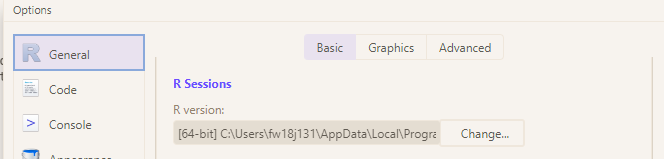
\includegraphics[keepaspectratio]{Plots/setRversion.png}}
\item
  Verwendet zum Installieren der Pakete den Code-Absatz aus der
  Einleitung. Die Pakete Laden Befehle aus den anderen Kapiteln sind
  nicht immer vollständig.
\end{itemize}

\section{Probleme beim Öffnen des
R-Projekts}\label{probleme-beim-uxf6ffnen-des-r-projekts}

Öffnet sich das R-Projekt gar nicht, leer, oder meldet Fehler bezüglich
der Schreibberechtigung, wurde möglicherweise die Übungs-.zip Datei
nicht korrekt entpackt. Stellt sicher, dass ihr die .zip Datei erst
entpackt und dann öffnet, anstatt das R-Projekt direkt aus der .zip
Datei zu öffnen.

\subsection{\texorpdfstring{\textbf{Windows}}{Windows}}\label{windows}

\begin{enumerate}
\def\labelenumi{\arabic{enumi}.}
\item
  \textbf{Rechtsklick auf die .zip-Datei}
\item
  Wähle \textbf{``Alle extrahieren\ldots{}''}
\item
  Wähle den gewünschten Speicherort und klicke auf
  \textbf{``Extrahieren''}
\end{enumerate}

\textbf{Alternative:} Falls kein „Alle extrahieren\ldots`` erscheint,
kannst du die Datei mit Programmen wie \textbf{7-Zip} entpacken.

\subsection{\texorpdfstring{\textbf{Mac
(macOS)}}{Mac (macOS)}}\label{mac-macos}

\begin{enumerate}
\def\labelenumi{\arabic{enumi}.}
\tightlist
\item
  \textbf{Doppelklick auf die .zip-Datei}\\
  → Der Ordner wird automatisch entpackt und erscheint im selben
  Verzeichnis.
\end{enumerate}

Falls der Doppelklick nicht funktioniert:

\begin{itemize}
\tightlist
\item
  Rechtsklick → \textbf{``Öffnen mit''} →
  \textbf{``Archivierungsprogramm''}
\end{itemize}




\end{document}
